%%%%%%%%%%%%%%%%%%%%%%%%%%%%%%%%%%%%%%%%%
% Thesis 
% LaTeX Template
% Version 1.3 (21/12/12)
%
% This template has been downloaded from:
% http://www.latextemplates.com
%
% Original authors:
% Steven Gunn 
% http://users.ecs.soton.ac.uk/srg/softwaretools/document/templates/
% and
% Sunil Patel
% http://www.sunilpatel.co.uk/thesis-template/
%
% License:
% CC BY-NC-SA 3.0 (http://creativecommons.org/licenses/by-nc-sa/3.0/)
%
% Note:
% Make sure to edit document variables in the Thesis.cls file
%
%%%%%%%%%%%%%%%%%%%%%%%%%%%%%%%%%%%%%%%%%

%----------------------------------------------------------------------------------------
%	PACKAGES AND OTHER DOCUMENT CONFIGURATIONS
%----------------------------------------------------------------------------------------

\documentclass[11pt, a4paper, oneside]{Thesis} % Paper size, default font size and one-sided paper

\graphicspath{{./Pictures/}} % Specifies the directory where pictures are stored
\usepackage{pgfplots}
\usepackage{morefloats}
\usepackage{enumerate}
\usepackage{tikz}
\usetikzlibrary{shapes,shadows,arrows}
\usepackage{rotating}
\usepackage{pdflscape}
\usepackage[square, numbers, comma, sort&compress]{natbib} % Use the natbib reference package - read up on this to edit the reference style; if you want text (e.g. Smith et al., 2012) for the in-text references (instead of numbers), remove 'numbers' 
\hypersetup{urlcolor=blue, colorlinks=true} % Colors hyperlinks in blue - change to black if annoying
\title{\ttitle} % Defines the thesis title - don't touch this

\begin{document}

\frontmatter % Use roman page numbering style (i, ii, iii, iv...) for the pre-content pages

\setstretch{1.3} % Line spacing of 1.3

% Define the page headers using the FancyHdr package and set up for one-sided printing
\fancyhead{} % Clears all page headers and footers
\rhead{\thepage} % Sets the right side header to show the page number
\lhead{} % Clears the left side page header

\pagestyle{fancy} % Finally, use the "fancy" page style to implement the FancyHdr headers

\newcommand{\HRule}{\rule{\linewidth}{0.5mm}} % New command to make the lines in the title page

% PDF meta-data
\hypersetup{pdftitle={\ttitle}}
\hypersetup{pdfsubject=\subjectname}
\hypersetup{pdfauthor=\authornames}
\hypersetup{pdfkeywords=\keywordnames}

%----------------------------------------------------------------------------------------
%	TITLE PAGE
%----------------------------------------------------------------------------------------

\begin{titlepage}
\begin{center}

\textsc{\LARGE Carleton University}\\[1.5cm] % Carleton University
\textsc{\Large Master's Thesis}\\[0.5cm] % Thesis type

\HRule \\[0.4cm] % Horizontal line
{\huge \bfseries Simulation of an Organic Memristor}\\[0.4cm] % Thesis title
\HRule \\[1.5cm] % Horizontal line
 
\begin{minipage}{0.4\textwidth}
\begin{flushleft} \large
\emph{Author:}\\
{Cem Bonfil} % Author name - remove the \href bracket to remove the link
\end{flushleft}
\end{minipage}
\begin{minipage}{0.4\textwidth}
\begin{flushright} \large
\emph{Supervisor:} \\
{Dr. Tom Smy}\\ % Supervisor name - remove the \href bracket to remove the link  
{Dr. Steven P. McGarry}
\end{flushright}
\end{minipage}\\[3cm]
 
\large \textit{A thesis submitted in fulfilment of the requirements\\ for the degree of Master's of Science in Electrical and Computer Engineering }\\[0.3cm] % University requirement text
\textit{in the}\\[0.4cm]
Carleton University\\[2cm] % Research group name and department name

{\large \today}\\[4cm] % Date

\includegraphics[scale=0.25]{Logo.png} % University/department logo - uncomment to place it

\vfill
\end{center}

\end{titlepage}

%----------------------------------------------------------------------------------------
%	DECLARATION PAGE
%	Your institution may give you a different text to place here
%----------------------------------------------------------------------------------------



%----------------------------------------------------------------------------------------
%	QUOTATION PAGE
%----------------------------------------------------------------------------------------

\pagestyle{empty} % No headers or footers for the following pages

\null\vfill % Add some space to move the quote down the page a bit

\textit{"Quote"}

\begin{flushright}
Cem Bonfil
\end{flushright}

\vfill\vfill\vfill\vfill\vfill\vfill\null % Add some space at the bottom to position the quote just right

\clearpage % Start a new page

%----------------------------------------------------------------------------------------
%	ABSTRACT PAGE
%----------------------------------------------------------------------------------------

\addtotoc{Abstract} % Add the "Abstract" page entry to the Contents

\abstract{\addtocontents{toc}{\vspace{1em}} % Add a gap in the Contents, for aesthetics

The Thesis Abstract is written here (and usually kept to just this page). The page is kept centered vertically so can expand into the blank space above the title too\ldots
}

\clearpage % Start a new page

%----------------------------------------------------------------------------------------
%	ACKNOWLEDGEMENTS
%----------------------------------------------------------------------------------------

\setstretch{1.3} % Reset the line-spacing to 1.3 for body text (if it has changed)

\acknowledgements{\addtocontents{toc}{\vspace{1em}} % Add a gap in the Contents, for aesthetics

The acknowledgements and the people to thank go here, don't forget to include your project advisor\ldots
}
\clearpage % Start a new page

%----------------------------------------------------------------------------------------
%	LIST OF CONTENTS/FIGURES/TABLES PAGES
%----------------------------------------------------------------------------------------

\pagestyle{fancy} % The page style headers have been "empty" all this time, now use the "fancy" headers as defined before to bring them back

\lhead{\emph{Contents}} % Set the left side page header to "Contents"
\tableofcontents % Write out the Table of Contents

\lhead{\emph{List of Figures}} % Set the left side page header to "List of Figures"
\listoffigures % Write out the List of Figures

\lhead{\emph{List of Tables}} % Set the left side page header to "List of Tables"
\listoftables % Write out the List of Tables

%----------------------------------------------------------------------------------------
%	ABBREVIATIONS
%----------------------------------------------------------------------------------------

\clearpage % Start a new page

\setstretch{1.5} % Set the line spacing to 1.5, this makes the following tables easier to read

\lhead{\emph{Abbreviations}} % Set the left side page header to "Abbreviations"
\listofsymbols{ll} % Include a list of Abbreviations (a table of two columns)
{
BTE & Boltzmann Transport Equations \\
CFL &  Courant-Friedrichs-Lewy \\
$ClO_4^-$ & Perchlorate \\
DD &  Drift Diffusion\\
FD &  Finite Difference\\
$Li^+ $ &  Lithium\\
PEDOT & Poly(3,4-ethylenedioxythiophene) \\
PSS & Poly(styrenesulfonate) \\
SG & Scharfatter-Gummel \\
%\textbf{Acronym} & \textbf{W}hat (it) \textbf{S}tands \textbf{F}or \\
}

%----------------------------------------------------------------------------------------
%	PHYSICAL CONSTANTS/OTHER DEFINITIONS
%----------------------------------------------------------------------------------------

\clearpage % Start a new page

\lhead{\emph{Physical Constants}} % Set the left side page header to "Physical Constants"

\listofconstants{lrcl} % Include a list of Physical Constants (a four column table)
{
% Constant Name & Symbol & = & Constant Value (with units) \\
Boltzmann Constant & k & = & 8.6173324 $10^{-5} $ eV/K \\
Elementary Charge & q & = &  1.6021765 $10^{-19} $ C \\
Vacuum Permittivity  & $\epsilon_0$ & = & 8.8541878 $10^{-12} $ F/m \\ 
}

%----------------------------------------------------------------------------------------
%	SYMBOLS
%----------------------------------------------------------------------------------------

\clearpage % Start a new page

\lhead{\emph{Symbols}} % Set the left side page header to "Symbols"

\listofnomenclature{lll} % Include a list of Symbols (a three column table)
{

% Symbol & Name & Unit \\
 D & Diffusivity & $m^2/s$ \\
 E & Electric Field & $V/m$ \\
 h & Unit Distance & $m$ \\
 I & Current & $A$ \\
 J & Current Density & $A/m^2$ \\
 $L_D$ & Debye Length & m \\
 $l_f$ & Mean Free Path & m \\
 M & Memristance & $\Omega$ \\
n & Electron Density & $m^{-3}$ \\
$N_A $ & Acceptor Density & $m^{-3}$ \\
$N_D $ & Donor Density & $m^{-3}$ \\
 $n_i$ & Intrinsic Carrier Density & $m^{-3}$ \\
  T & Temperature & $K$  \\
  t & Time & $s$ \\
   $t_{dr}$ & Dielectric Relaxation Time & $s$ \\
   U & Generation Recombination Rate & $m^{-3}s^{-1}$ \\
   V & Potential & $V$ \\
   $V_{th}$ & Thermal Voltage & V \\

& & \\ % Gap to separate the Roman symbols from the Greek
% Symbol & Name & Unit \\
$\Delta$ & Unit Distance & $m$ \\
$\varepsilon_r$ & Relative Permittivity & unitless \\
$\mu$ & Mobility & $m^2/(Vs)$ \\
$\varphi$ & Flux Linkage & $Wb$ \\
$\rho$ & Charge Density & $C/m^3$ \\
$\upsilon$ & Drift Speed & $m/s$ \\
}

%----------------------------------------------------------------------------------------
%	DEDICATION
%----------------------------------------------------------------------------------------

\setstretch{1.3} % Return the line spacing back to 1.3

\pagestyle{empty} % Page style needs to be empty for this page

\dedicatory{For/Dedicated to/To my\ldots} % Dedication text

\addtocontents{toc}{\vspace{2em}} % Add a gap in the Contents, for aesthetics

%----------------------------------------------------------------------------------------
%	THESIS CONTENT - CHAPTERS
%----------------------------------------------------------------------------------------

\mainmatter % Begin numeric (1,2,3...) page numbering

\pagestyle{fancy} % Return the page headers back to the "fancy" style

% Include the chapters of the thesis as separate files from the Chapters folder
% Uncomment the lines as you write the chapters

% Chapter 1

\chapter{Introduction} % Main chapter title


\label{Chapter1} % For referencing the chapter elsewhere, use \ref{Chapter1} 

\lhead{Chapter 1. \emph{Introduction}} % This is for the header on each page - perhaps a shortened title

\section{Thesis Objectives}
\begin{doublespace}
The purpose of this thesis is to create a numerical simulation which captures the physics behind the operation of a memristor based on an organic semiconductor. Proposed model can be used for researching the physics behind the actual device through further modeling or as a tool for designing memristors for a specific purpose. 

A simple memristor model is created using only the essential components and physical effects. A numerical solver for drift diffusion and poisson equations are developed and tested. A memristor simulation is created by modifying the drift diffusion solver to accommodate all the essential physical effects. Finally the simulation results are compared with experimental results from a memristor fabricated at Carleton University.

\section{Thesis Overview}

The discovery of the memristor and challenges in memristor research is introduced in the background chapter. It emphasizes the need for better physical modeling for the memristor and the lack of simulation tools required for further analysis and research.

In chapter 2 , Boltzmann Transport Equations (BTE) are introduced. This introduction is followed by the explanation of the transport mechanisms captured through BTE. Additionally drift diffusion equations (simplified form of BTE) which will be used for the simulation of the memristor are discussed. Finally various analytic solutions to drift diffusion equations, such as charged particles moving over an infinite conductor and a PN junction, are derived and plotted. 

A numerical solution to the drift diffusion equations is formed in chapter 3 to calculate the movement of all the charged particles in a memristor. First a finite difference method, which is the basis for all the simulations in this thesis is introduced. Then it is applied to drift diffusion equations. Additionally, a Poisson solver to be used with the drift diffusion equations is developed in order to calculate the electric field generated by charged particles and metal contacts. Boundary conditions necessary for the solution of both drift diffusion equations and Poisson solver are discussed. All the equations and boundary conditions combined generate a set of equations to be solved for the simulation of the memristor. Various schemes for solving these differential equations as well as numerical and physical limitations are discussed in detail.
 
In chapter 4, the numerical solver developed in chapter 3 is tested against analytic solutions as well as numerical solutions generated by a commercially available simulator called COMSOL Multiphysics. A mechanism to limit the maximum density of any particle, which is essential for memristor simulation, is developed and tested. 

After the stability and accuracy of the simulation scheme is tested in chapter 4, a memristor model is introduced in chapter 5. The difficulties in the simulation due to physical and numerical restrictions are discussed. A possible 1-D approximation for a 2-D memristor simulation is proposed and simulated. After demonstrating that the simulations produced reasonable results, the validity of the approximations made for 1-D and 2-D simulations are investigeted.  

A full 2-D simulation is discussed in chapter 6. A memristor with various PEDOT thicknesses are simulated. A memristor with various PEDOT:PSS thicknesses are simulated and compared to each other. The simulation with thinnest PEDOT is compared to 1-D simulations made in the previous chapter. Finally memristor simulations are compared against experimental data.

The conclusion chapter summarizes the findings of the thesis, discusses advantages and disadvantages of the proposed simulation methods and provides suggestions for improvements on the model and opportunities for further research.

\section{Contributions}

\begin{itemize}
  \item An organic memristor which is a charge dependent resistor is numerically modeled using drift diffusion equations  
  \item A special mechanism is developed to limit the amount of lithium ions that can accumulate inside the PEDOT:PSS
  \item Two different memristor structures,a single strip and a notched PEDOT:PSS, are simulated for various applied potentials
  \item Modeled behavior of the memristor is verified through experimental results 
\end{itemize}

\section{Background}
The term memristor was first used by Leon Chua in 1971 in his paper called  "Memristor — The Missing Circuit Element" \cite{chua}. He theorized that there is a fourth passive circuit element yet to be discovered in addition to resistor,capacitor and inductor. He said that we already know and use five out of six possible combinations that can be made out of four fundamental circuit variables, current \textit{I}, voltage \textit{V}, charge \textit{q} and flux linkage \textit{$\varphi$}. Chua claimed that there is missing a circuit element which produces a relationship between flux linkage(time integral of the potential) and charge. He introduced a new variable named memristance which has units of resistance and it is a function of charge. The relationship between the current and the potential of a memristor is calculated by replacing the resistance by memristance in ohms law:

 %\cite{chua} \cite{Dragica1} \cite{SG} \cite{NumModel} \cite{MisMem} \cite{SimChargeTrans} \cite{PedotBook} \cite{snowden} \cite{PedotCon}.

\begin{equation}
v(t)=M(q(t))i(t)
\end{equation}

Theoretically a memristor retains its resistance in the absence of any power source. When a potential is applied, the resistance can be influenced by the direction and the magnitude of the current. If the current flows in one direction the resistance increases and if it flows in the other direction the resistance decreases. This produces an I-V response which looks like a pinched hysteresis curve. This response is the main characteristic of a memristor. 

This new element remained mostly a theory and it did not get a lot of academic attention until a group of researchers in Hewlett Packard developed a fully functioning memristor \cite{MisMem}. They successfully fabricated a nano scale memristor using $TiO_2$ (titanium dioxide). After the discovery in HP labs there was an increase of interest in different types of memristors due to their potential applications for data storage and the addition of learning capabilities into passive circuits \cite{AdaptiveMem} \cite{Synapse} \cite{CMOS}. 

Recently it has been suggested that organic based memristors could be fabricated \cite{OrganicMem}. This thesis will be concerned with such devices. They are usually constructed on a larger scale than the ones fabricated in HP labs. The memristor studied in this thesis is in millimeter rather then nano meter scale and uses a conductor made out of a polymer called PEDOT:PSS. It is composed of two polymer chains, PEDOT and PSS attached together and conducts electricity via hole transport. Unfortunately the conduction mechanism is not perfectly understood and needs further research due to the complexity of the material \cite{PedotBook}.

Unlike a semiconductor like silicon, the structure of a polymer is quite irregular \cite{PedotBook}. Polymers have individual molecules with different chain lengths and a variable amount of defects. Additionally, they can be amorphous or partially crystalline and further differences occur through aging. The conduction and the electronic properties depend on the orientation of the polymer chains which can change in x,y and z directions. These irregularities in the structure makes these conducting polymers resemble amorphous inorganic semiconductors. Following the concept of charge transport in amorphous inorganic semiconductors, the conduction mechanism of conducting polymers is commonly explained by variable range hopping. This mechanism was first introduced by Mott\cite{Mott}. He proposed a model for charge transport in systems that are randomly disordered. In variable range hopping, charge transport occurs via jumps between available sites. Every charge carrier has a probability of jumping between two sites depending on its energy and the distance to the next available site. The temperature has a big impact on conductivity since it changes the structure of the molecules and increases the energy of charge carriers.

Apart from the temperature there are other ways to influence the conductivity of PEDOT. It is possible to affect the conductivity by either doping or counter doping \cite{PedotDope}. Depending on the method used, doping can be reversible or permanent. When reversible doping is employed, the resulting device behaves like a memristor since its resistance is now dependent on charge. All these effects make physical modeling, experimentation and simulation very challenging. 

There are a few compact models for inorganic memristors similar to the one produced in HP labs \cite{ChuaSim}\cite{MemCircuitSim}. These solutions are mostly based on parameter fitting and some basic physics. Studies on organic memristors are more sparse than studies on inorganic ones and a standard method for simulating organic memristors is not developed. The physics behind the conduction mechanism and the changes in the conductivity due to doping requires further research and the development of a computer model can help in various ways. It is very difficult to get experimental data on the movement of ions and holes inside the PEDOT:PSS due to its disordered structure. Theories that explain the movement of charged particles and their interactions with each other are difficult to formulate since it is hard to obtain required experimental data. A simulator can be a useful tool in testing various theories without having to set up and perform complicated experiments. Also once a solid understanding of the conduction mechanism is achieved and a reliable memsristor model is developed, simulations can be very useful to test different device structures and optimize them before fabrication. 


 \end{doublespace}
% Chapter Template

\chapter{Theory} % Main chapter title

\label{Chapter2} % Change X to a consecutive number; for referencing this chapter elsewhere, use \ref{ChapterX}

\lhead{Chapter 2. \emph{Theory}} % Change X to a consecutive number; this is for the header on each page - perhaps a shortened title
\begin{doublespace}
The memristor studied in this thesis uses a strip of PEDOT:PSS as a conductor. A drop of an electrolytic solution which has lithium and perchlorate ions is placed on top of this conducting strip. When a potential is applied, lithium ions inside the electrolyte solution migrate into PEDOT:PSS and modifiy its conductivity. Hole transport inside PEDOT:PSS as well as lithium and perchlorate movement are modeled using basic drift diffusion equations which are derived in the first part of this chapter. The second half of the chapter shows analytic solutions to drift diffusion equations which will be used to test the numerical methods derived in the following chapter.


\section{Carrier Transport Equations}
Drift diffusion equations, which are based on BTE\cite{Dragica1}, need to be solved in order to model the complex behaviour of the memristor. Drift-diffusion equations are derived by simplifying BTE equation via approximations. These simplifications dictate the limits of the drift-diffusion model, therefore they need to be well understood.

The derivation of Boltzmann transport equation starts by stating that a distribution of charged particles can be defined by their position in space \textbf{r} and momentum \textbf{k} in time \textbf{t} using a probability distribution function f(k,r,t). This results in the most general form of Boltzmann transport equation.

\begin{equation}
\frac{d }{dt}f(k,r,t)=0
\end{equation}

This general form of BTE needs to be expanded and relevant physical equations need to be placed in to get an equation describing a specific problem or a device. 
Many different device simulators use some sort of approximation to BTE. In semiconductor simulations they are commonly used for the movement of charge carriers such as holes (p) and electrons (n). 

After this brief introduction to BTE, rather than going through the mathematical derivation of the drift diffusion model, the approximations that are made along the process of derivation are discussed in order to get a better insight on the model.  As a particle travels in a solid state device it collides with other particles as well as the atoms in the device. For drift-diffusion equations individual lattice scattering events or collisions are averaged and all the particles have an average constant velocity under the effects of an electric field \cite{snowden}. This means that all the particles respond instantaneously to the changes in the electric field. The movement of the particles due to the electric field is called the drift current. The relationship between the drift velocity and the electric field is given by the following equation:

\begin{equation}
v=\mu E
\end{equation}

$\mu$ is called the mobility constant and it determines the speed at which the particles are going to move when subject to an electric field. Drift current density can be derived based on drift velocity.

\begin{equation}
J_E=q n\mu E=q n v 
\end{equation}

Where q is the elementary charge and n is the electron density. In addition to the previous assumptions, it is assumed that the lattice is perfectly uniform, has a uniform temperature distribution and all the temperature of the particles are close to the temperature of the lattice. Based on this assumption it is possible say that all the particles move due to thermal effects with the same thermal velocity ($v_{th}$) and mean free path ($l_f$). These quantities can be combined into one single coefficient called the diffusion constant. 

\begin{equation}
D=v_{th} \;l_f
\end{equation}

Drift and diffusion coefficients are related to each other via the Einstein relationship\cite{snowden}:

\begin{equation}
D=\frac{\mu k T}{q}
\end{equation}

Where k is the Boltzmann constant and T is the lattice temperature. The random thermally driven motion produces diffusion and results in a second term which contributes to the carrier movement and it is called the diffusion current density.

\begin{equation}
J_D=qD\frac{dn}{dx}
\end{equation}

Unlike the drift current density, which is directly related to the carrier density, diffusion current density is related to the carrier density's first order derivative in space. Combining these two terms results in the following the current density equation for electrons in one dimension.

\begin{equation}
\vec{J_n^x}=q \mu_{n} n \vec{E_x}+qD_{n} \frac{dn}{dx} 
\label{cdenn}
\end{equation}

This equation can be easily extended to other dimensions by simply using the appropriate terms.

\begin{equation}
\vec{J_n^y}=q \mu_{n} n \vec{E_y}+qD_{n} \frac{dn}{dy} 
\end{equation}

The current density equations can be used for both positively and negatively charged particles by changing the sign of the diffusion current density.

\begin{equation}
\vec{J_p^x}=q \mu_{p} p \vec{E_x}-qD_{p} \frac{dp}{dx} 
\label{cdenp}
\end{equation}
Anisotropic drift and diffusion coefficients can be handled with ease by using different coefficients for different directions. Also the mobility and the diffusivity can be a function of any variable such as position or temperature. This is a useful property for a memristor simulation since hole mobility depends on lithium density in the PEDOT:PSS at any given position. 

Current density equations by themselves are not enough to solve this time dependent problem. It is necessary to account for the movement of charge over time which is captured in the continuity equation. It is a statement of conservation of particle density over time. The change in the amount of carriers over time in a particular area must be equal to the difference in current density over the same area. Additionally the amount of charge can change due to generation-recombination of charged particles. The continuity is captured by equations:


\begin{equation}
\frac{\partial n}{\partial t}=\frac{1}{q}\nabla \cdot \vec{J_n}+U_{n}
\label{conn}
\end{equation}

\begin{equation}
\frac{\partial p}{\partial t}=-\frac{1}{q}\nabla \cdot \vec{J_p}+U_{p}
\label{conp}
\end{equation}

$U_{n}$ and $U_{p}$ are net generation recombination rates. These terms were not included in the modeling of the memristor. 

Electric field can be generated in two different ways. One is through the distribution of net charge over the area and the other one is an externally applied potential. It is possible to calculate the potential distribution over an area by using Poisson's equation \cite{Dragica1}. Once the potential is known the electric field can be obtained by just calculating the negative gradient of the electric potential.

\begin{equation}
\nabla \cdot  (\varepsilon \nabla V)=-\rho=-q(p-n+N_{D}^{+}-N_{A}^{-})
\label{poisson}
\end{equation}
\begin{equation}
\vec{E}=-\nabla V
\label{Efield}
\end{equation}

The electric field can be split into multiple components depending on the dimensions of the problem. In a 2-D case they are $\vec{E_x}$ and $\vec{E_y}$.

\begin{equation}
\vec{E_x}=-\frac{\partial V}{\partial x}
\end{equation}

\begin{equation}
\vec{E_y}=-\frac{\partial V}{\partial y}
\end{equation}

Once the electric field and the current density is known, the current at any point in the device can be easily calculated by using the following integral \cite{snowden}.

\begin{equation}
I=\int\limits_{s}^{}\vec{J_{tot}} \cdot ds = \int\limits_{s}^{}(J_n+J_p+\varepsilon\frac{\partial E}{\partial t})ds
\end{equation}

Poisson's equation and drift-diffusion equations are coupled through the electric field and net charge distribution. The strength of this non linear coupling depends on the size of the device and the charge density which determines the total amount of charge over an area. In a strongly coupled system of differential equations, small changes in either the charge density or the electric field can easily cause instabilities in the simulation. This is further discussed in the next chapter while developing a numerical scheme to solve the system of equations described in this chapter. 

Drift diffusion equations derived above hold for the ions in the electrolyte as long as fluid effects can be ignored. For the memristor simulated in this thesis, there are three distinct types of mobile particles, holes, lithium and perchlorate. In PEDOT:PSS there is also a finite amount of negatively charged particles which are immobile, therefore they are only included in Poisson's equation. The main equations for the drift-diffusion model that are used for the memristor simulation can be compactly written as:

\begin{equation}
\nabla \cdot  (\varepsilon \nabla V)=-q(p-n+N_{D}^{+}-N_{A}^{-})
\end{equation}
\begin{equation}
\vec{J_p}=q\mu_p p \vec{E}-q D_p \nabla p
\end{equation}
\begin{equation}
\vec{J_{N_{A}^{-}}}=q\mu_{N_{A}^{-}} N_{A}^{-} \vec{E}+q D_{N_{A}^{-}} \nabla N_{A}^{-}
\end{equation}
\begin{equation}
\vec{J_{N_{D}^{+}}}=q\mu_{N_{D}^{+}} N_{D}^{+} \vec{E}-q D_{N_{D}^{+}} \nabla N_{D}^{+}
\end{equation}
\begin{equation}
\frac{\partial p}{\partial t}=-\frac{1}{q}\nabla \cdot \vec{J_p}
\end{equation}
\begin{equation}
\frac{\partial N_{A}^{-}}{\partial t}=\frac{1}{q}\nabla \cdot \vec{J_{N_{A}^{-}}}
\end{equation}
\begin{equation}
\frac{\partial N_{D}^{+}}{\partial t}=-\frac{1}{q}\nabla \cdot \vec{J_{N_{D}^{+}}}
\end{equation}

This system of equations consist of 4 different charge carriers. There are 3 mobile species lithium ($N_{D}^{+}$) and perchlorate ($N_{A}^{-}$) and holes (p) and one fixed charge, electrons (n). The particles are coupled to each other through Poisson's equation since they all carry electric charge. 

Even after many approximations to the BTE, the drif diffusion equations have analytical solutions for only few isolated cases. The analytical solutions developed in the rest of this chapter are used in the testing of the numerical method developed for simulating a memristor. 

\clearpage
\section{Analytic Solutions}

Three different analytic solutions to drift diffusion equations will be developed in this section. It starts with a simple steady state problem with uniform electric field. The second example, which is more complex than the first one, is a transient solution for a charge distribution moving under uniform electric field. Finally, a PN junction problem is solved which incorporates the drift diffusion equation with Poisson's equation and provides a steady state solution for electron/hole density distributions, potential and electric field. 
  
\subsection{Steady State Solution Over a Finite Domain}

The problem that will be solved in this section consists of a finite amount of charge and a uniform electric field pushing this charge against a wall. It is assumed that the charge density is low enough not to affect the uniform electric field, therefore the solution of Poisson's equation is not necessary. To simplify the problem even further only a steady state solution is derived. Also it is important to note that the initial distribution of the charge density does not matter in this problem since all the charge will be redistributed in steady state. The only relevant information is the total amount of charge subject to the electric field. At steady state, drift and diffusion currents are in equilibrium and net current density is zero. Following equation shows the hole current density at equilibrium:

\begin{equation}
J_p(x)=q \mu_{p} p E-qD_{p} \frac{dp}{dx} =0
\end{equation}

Total current density will only be zero when the drift current density generated by the electric field is completely balanced by the diffusion current density.

\begin{equation}
q \mu_{p} p E=qD_{p} \frac{dp}{dx}
\end{equation}

\begin{equation}
 \frac{\mu_{p} E}{D_{p}} p  = \frac{dp}{dx}
 \label{pdif}
\end{equation}

This is a simple differential equation that can be solved by assuming that hole density has the following form:

\begin{equation}
p(x)=Ce^{ax}
\label{px}
\end{equation}

\textbf{C} and \textbf{a} are arbitrary constants. Equation \eqref{px} can be placed into \eqref{pdif}.

\begin{equation}
 \frac{\mu_{p} E}{D_{p}} Ce^{ax}  = a Ce^{ax}
\end{equation}

\begin{equation}
a=\frac{\mu_{p} E}{D_{p}}
\end{equation}

 A general form for the solution is generated by placing \textbf{a} back into equation \eqref{px}.
 
\begin{equation}
p(x)=Ce^{\frac{\mu_{p} E}{D_{p}}x}
\label{p_ss}
\end{equation}

It is possible to solve for \textbf{C} by observing that the total amount of charge at steady state must be equal to the initial amount of charges since all the holes remain inside the conductor. So the integral of the initial hole density distribution must be equal to the integral of the charge density at steady state.


\begin{equation}\nonumber
\int\limits_{0}^{L}Ce^{\frac{\mu_{p} E}{D_{p}}x}dx=\int\limits_{0}^{L}p(t=0,x)dx
\end{equation}

\begin{equation}\nonumber
C=\frac{\int\limits_{0}^{L}p(t=0,x)dx}{\int\limits_{0}^{L}e^{\frac{\mu_{p} E}{D_{p}}x}dx}
\end{equation}

\begin{equation}
C=\frac{\int\limits_{0}^{L}p(t=0,x)dx}{\frac{D_p}{\mu_p E}[e^{\frac{\mu_p E}{D} L} -1]}
\label{p_ss_c}
\end{equation}

Equation \ref{p_ss} combined with equation \ref{p_ss_c} gives a complete solution for this problem which shows that increasing the electric field will concentrate the charge density at the edge of the conductor. Physically this behavior is reasonable, since the force that is pushing the particles against a wall is getting greater and it is making the charges accumulate even more. Following plot demonstrates the affect of the electric field on the hole distribution.

\begin{figure}[!htp]
\centering
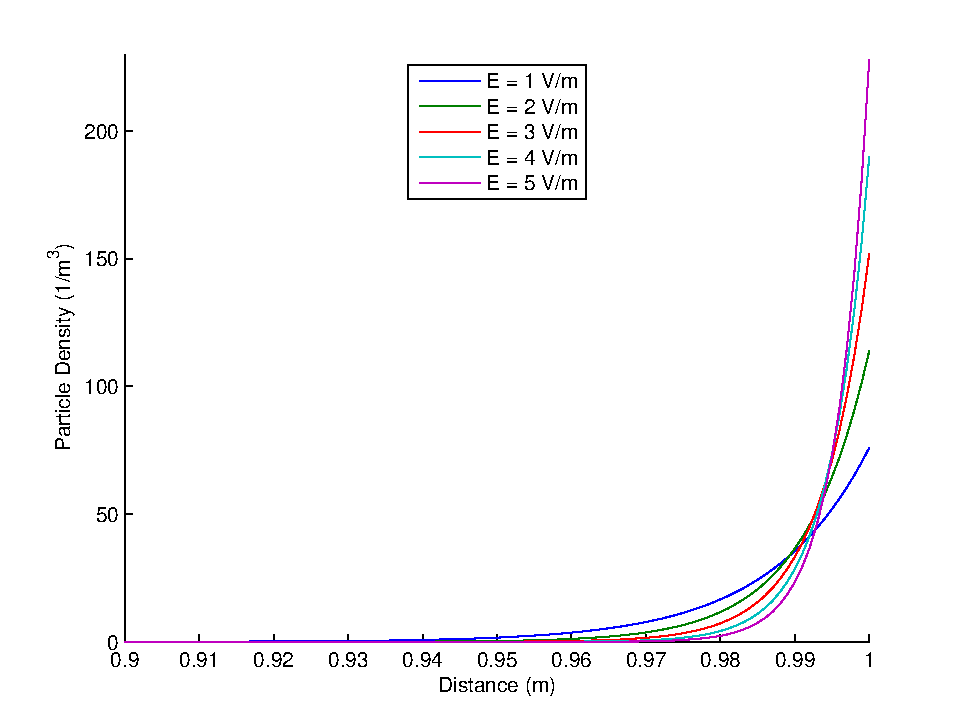
\includegraphics[scale=0.7]{AnalyticSS}
\caption{Increased accumulation of particles due to increased electric field} 
\end{figure}

Debye length is the length over which mobile charge carriers screen out an external electric field and it determines how steeply charges will accumulate over a certain distance. This example also illustrates the decrease in the debye length due to the increase in the charge density. Debye length is determined by the strength of the electric field created by the charge present in the material. The increase in the electric field in this example is analogous to the increase in charge density. Increased charge density creates a larger electric field. This creates a steeper accumulation of the charged particles and a decrease in the debye length. 

\clearpage
\subsection{Transient Solution Over an Infinite Domain}

The problem that is solved in this section consists of an initial particle density distribution subject to a uniform electric field over an infinitely long conductor. The charge distribution drifts and diffuses over time. This requires a transient solution and the continuity equation (\ref{conn}) needs to be solved. Again, charged particles do not affect the electric field therefore solution of Poisson's equation is not necessary. 

The first step of the solution process is the insertion of \eqref{cdenn} into \eqref{conn}.

\begin{equation}
\frac{\partial n}{\partial t} = \frac{1}{q}\nabla \cdot (\vec{J_n})
\end{equation}


\begin{equation}
\frac{\partial n}{\partial t} = \frac{1}{q}\nabla \cdot (q \mu_{n} n \vec{E}+qD_{n} \frac{dn}{dx} )
\end{equation}

For 1-D this can be simplified to:
\begin{equation}
\frac{\partial n}{\partial t} = \mu_n E \frac{d n}{d x}+D_{n}\frac{d^{2}n}{dx^{2}}
\label{adifg}
\end{equation}

Using separation of variables the solution can be separated into time and space dependent functions.
\begin{equation}
n(t,x)=n(t)n(x)=n_t n_x
\label{adifn}
\end{equation}
Placing equation \eqref{adifn} into \eqref{adifg} and dividing by n(t,x),
\begin{equation}
\frac{1}{n_{t}}\frac{d n_{t}}{d t}=\mu_n E \frac{1}{n_{x}}\frac{d n_{x}}{dx}+D\frac{1}{n_{x}}\frac{d^2 n_{x}}{dx^2}
\label{Adif}
\end{equation}
Assuming both sides of the equation are equal to a constant -k, time dependent part of the problem becomes a simple first order differential equation.

\begin{equation}
\nonumber
\frac{1}{n_{t}}\frac{d n_{t}}{dl t}=-k
\end{equation}

\begin{equation}
\nonumber
\frac{d n_{t}}{d t}=-kn_t
\end{equation}

Based on the above differential equation $n_t$ can take the following form:

\begin{equation}
n_t=C_1 e^{-kt}
\label{nt}
\end{equation}

Now for $n_x$ assuming a solution of the form below,

\begin{equation}
n_x=C_2 e^{-j\omega x}
\label{nx}
\end{equation}

Placing \eqref{nx} into \eqref{Adif}

\begin{equation}
\omega^2 D C_2 e^{-j\omega x}-j\omega \mu_n E C_2 e^{-j\omega x}+kC_2e^{-j\omega x}=0
\label{omegak}
\end{equation}

Simplifying equation \eqref{omegak} and solving for k gives,

\begin{equation}
k=\omega^2 D+j\omega \mu_n E
\label{k}
\end{equation}

Combining equation \eqref{nt}, \eqref{nx} and \eqref{k} to get the initial form of the solution. $(C=C_1C_2)$

\begin{equation}
n=n_tn_x=Ce^{(-\omega^2 D + j\omega \mu_n E)t} e^{-j\omega x}
\end{equation}

The application of the superposition principle leads to:

\begin{equation}
n=n_tn_x=\int\limits_{-\infty}^{\infty}C(\omega)e^{(-\omega^2 D + j\omega \mu_n E)t} e^{-j\omega x}d\omega
\label{nfinal1}
\end{equation}

The distribution of $n_x$ is known at t=0.

\begin{equation}
n(x,t=0)=\int\limits_{-\infty}^{\infty}C(\omega) e^{-j\omega x}d\omega
\end{equation}

$C(\omega)$ is just the inverse fourier transform of $n(x,0)$.

\begin{equation}
C(\omega)=\int\limits_{-\infty}^{\infty}n(x,0)e^{-j\omega x}dx
\label{comega}
\end{equation}

The final form of the solution is generated by placing equation \eqref{comega} into \eqref{nfinal1}:

\begin{equation}
n=\int\limits_{-\infty}^{\infty}\int\limits_{-\infty}^{\infty}n(z,0)e^{j\omega z}dz e^{(\omega ^2 D-j\omega \mu_n E)t}e^{-j\omega x}d\omega
\label{nfinal2}
\end{equation}

Rearranging equation \eqref{nfinal2},

\begin{equation}
n=\int\limits_{-\infty}^{\infty}\int\limits_{-\infty}^{\infty}n(z,0) e^{(\omega ^2 D-j\omega \mu_n E)t}e^{-j\omega x} e^{j\omega z}  dz d\omega
\end{equation}

Using a gaussian initial distribution results into:

\begin{equation}
n(x,0)=e^{- (\frac{x-x_o}{\sigma})^2}
\end{equation}

\begin{equation}
n(x,t)=\frac{1}{\sqrt{4D_n\sigma^{-2}t+1}}e^{-\frac{(t\mu_n E-x+x_o)^2}{4D_n t+\sigma^2}}
\end{equation}

If the initial distribution is a rectangular then the solution takes the following form:

\begin{equation}
n(x,0)=\prod (w(x))
\end{equation}

\begin{equation}
n(x,t)=\frac{1}{2} erf(\frac{w+2t \mu_n E-2x}{4\sqrt{D_n t}})-\frac{1}{2}erf(\frac{-w+2t \mu_n E-2x}{4\sqrt{D_n t}}) 
\end{equation}

Following plots show the evolution of two particle densities with different initial distributions described above.

\begin{figure}[!htp]
\centering
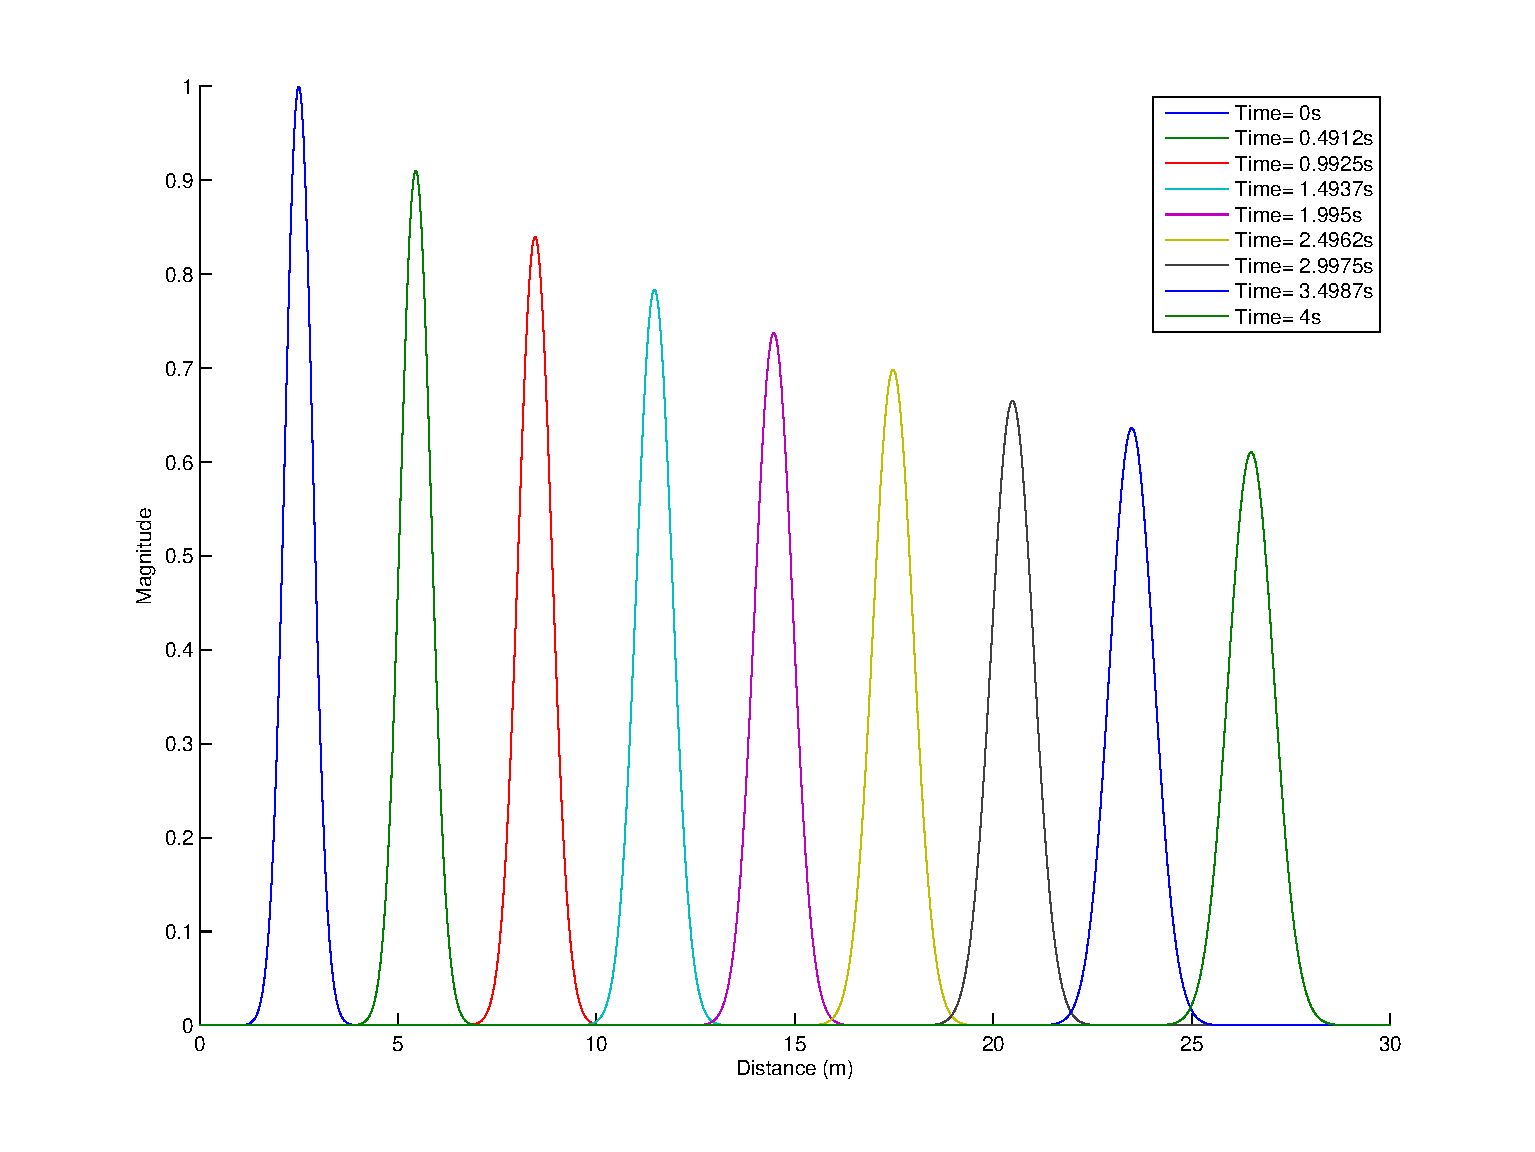
\includegraphics[scale=0.5]{AnalyticGauss}
\caption{A gaussian particle density distribution drifting and diffusing over time} 
\end{figure}

\begin{figure}[!htp]
\centering
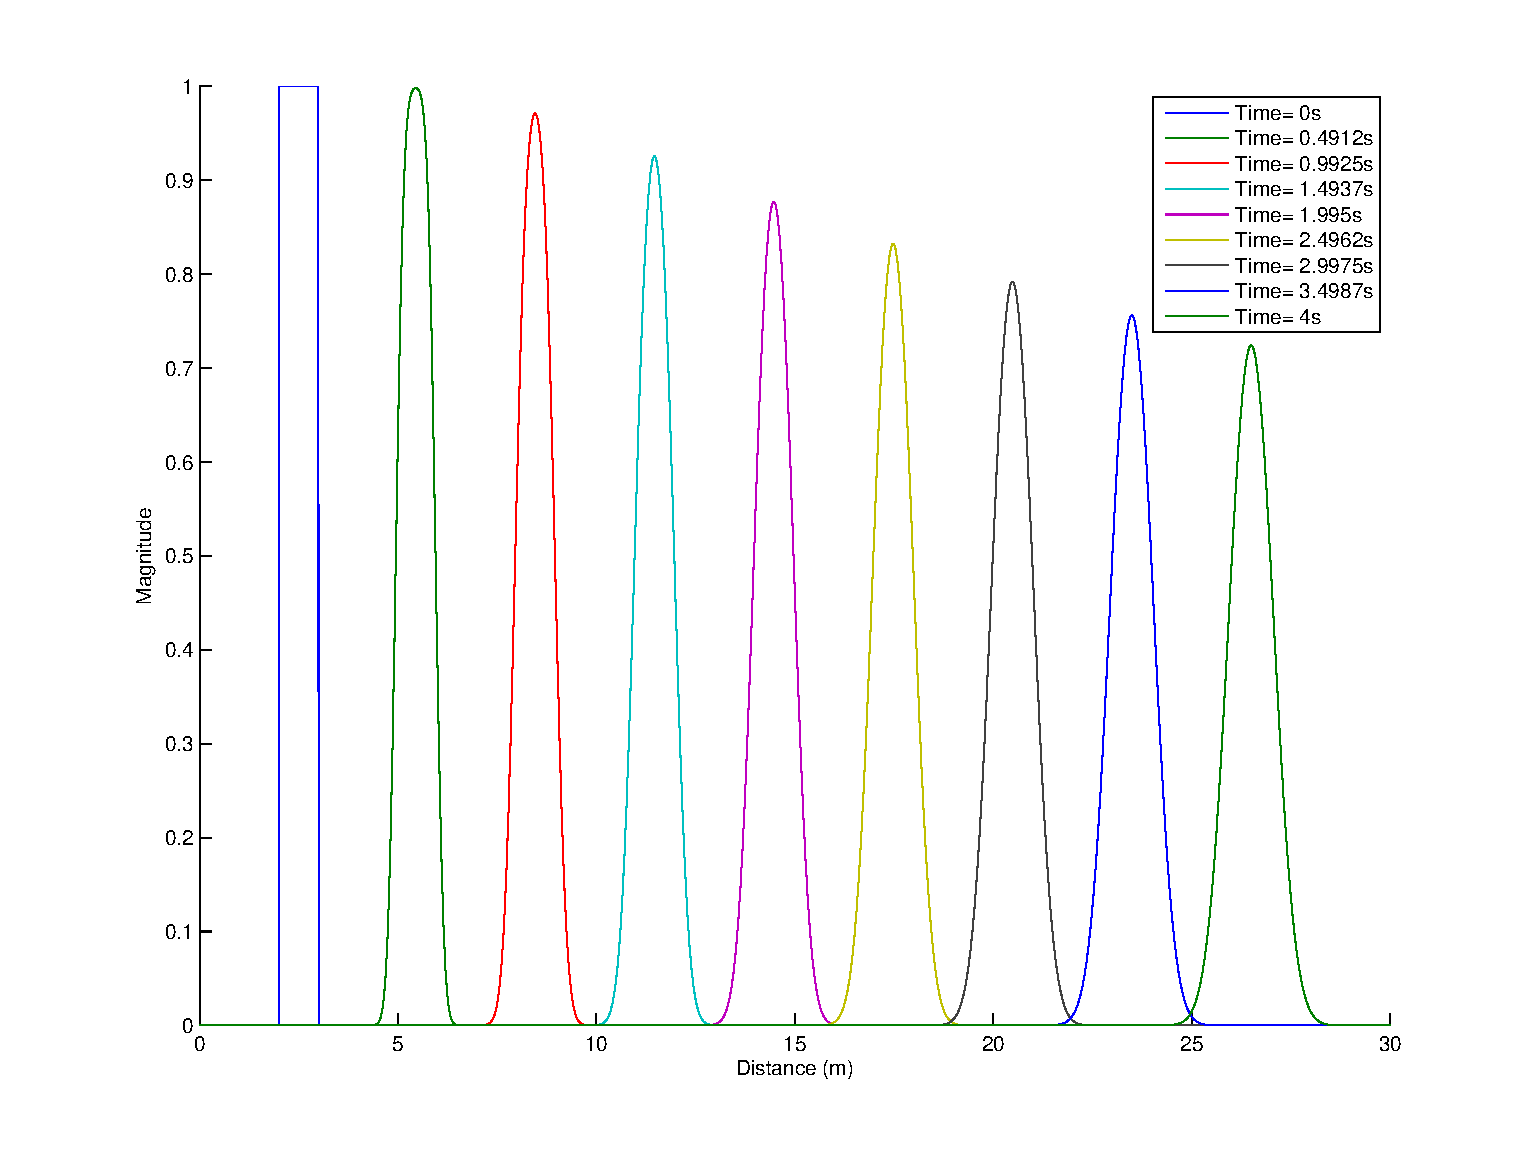
\includegraphics[scale=0.5]{AnalyticRect}
\caption{A rectangular particle density distribution drifting and diffusing over time} 
\end{figure}
\clearpage
\subsection{PN Junction}
Previous analytical solutions involved the solution of Poisson's equation and continuity equation which are not coupled. An example where these equations are tightly coupled is examined in this section. There are usually no direct analytical solutions for coupled equations but it is possible to get a closed form solution by making use of certain approximations. One example of this situation is an abrupt p-n junction. An abrupt p-n junction is created when two materials of opposite doping,p type and n type, are brought together. A p type material has an excess number of acceptors $N_A$ and an n type material has an excess number of donors $N_D$. The junction is defined at the interface where $N_A=N_D$ \cite{Physem}. 

\begin{figure}[!htp]
\centering
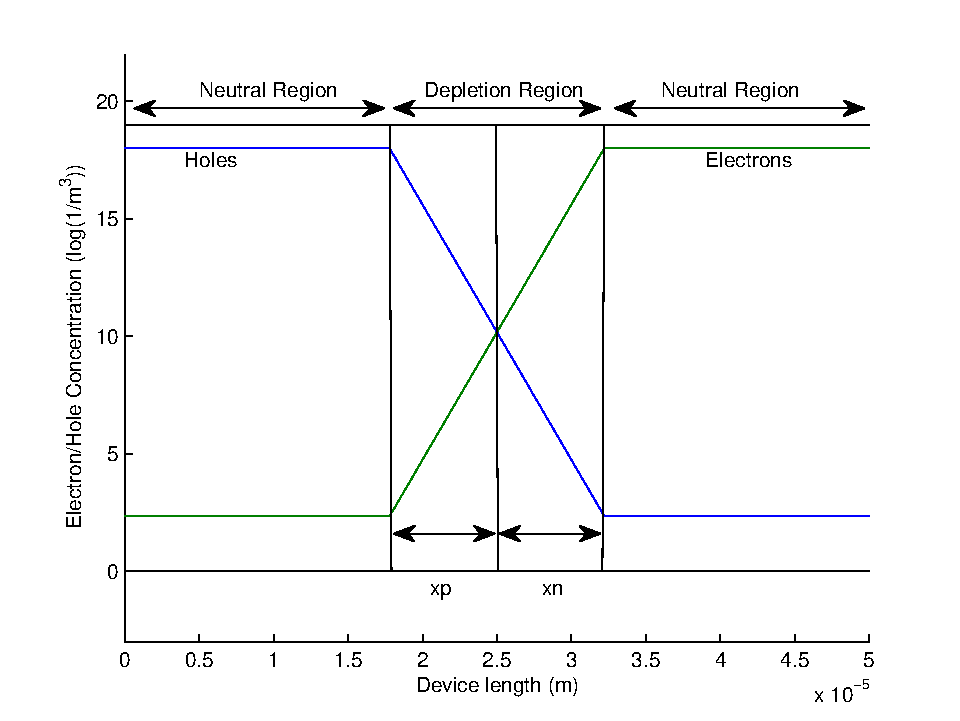
\includegraphics[scale=0.8]{3331}
\caption{PN junction electron/hole density} 
\end{figure}

In this example an analytical solution for an abrupt p-n junction is derived. To get a solution for this problem depletion region approximation is used. This approximation starts by assuming that the charges are fully depleted around the junction\cite{Physem}. All the electric field is confined in the depletion region and regions far away from the junction are neutral. Based on this, the net charge density over the entire region is:

\begin{equation}
\frac{d \vec{E} }{dx}=\frac{\rho}{\varepsilon}=\frac{q}{\varepsilon}(-N_{A}+N_{D})
\end{equation}

\begin{equation}
\rho = \begin{cases}
         0 & \text{for} \;  x<-x_{p}\\
       -qN_{A} & \text{for}  -x_{p}\leq x \leq 0 \\
        qN_{D} & \text{for} \; 0 \leq x \leq< x_{n}  \\
        0 & \text{for}\;  x>x_{n} \\
     \end{cases}
\end{equation}

The electric field over the entire region can be calculated by integrating $\rho$.

\begin{equation}
E = \begin{cases}
       \int \frac{-qN_{A}}{\varepsilon}  dx+ C_{1} & \text{for}  -x_{p}\leq x \leq 0 \\
       \int \frac{qN_{D}}{\varepsilon} dx+ C_{2}   & \text{for } \; 0 \leq x \leq x_{n}  \\
     \end{cases}
\end{equation}

It is possible to solve for $C_{1}$ and $C_{2}$ since electric field must go to zero at $x_{p}$ and $x_{n}$.

\begin{equation}
E(x=-x_{p})=0  \; \;  \Rightarrow  \;\; C_{1}= \frac{-qN_{A}}{\varepsilon}x_{p}
\end{equation}

\begin{equation}
E(x=x_{n})=0  \; \;  \Rightarrow  \;\; C_{1}= \frac{qN_{D}}{\varepsilon}x_{n}
\end{equation}

Then E(x) becomes:

\begin{equation}
E(x) = \begin{cases}
         \frac{-qN_{A}}{\varepsilon}(x+x_{p}) & \text{for}  -x_{p}\leq x \leq 0 \\
         \frac{qN_{D}}{\varepsilon}(x-x_{n})  &  \text{for} \; 0 \leq x \leq x_{n}  \\
     \end{cases}
\end{equation}
 Additionally, the electric field must be continuous across the interface therefore the electric field in the p-type side and the n-type side must equal each other at the interface or when x = 0. 

\begin{equation}
\frac{-qN_{A}}{\varepsilon}(x_{p})=\frac{qN_{D}}{\varepsilon}(-x_{n})
\end{equation}

\begin{equation}
N_{A}x_{p}=N_{D}x_{n}
\label{NAeqND}
\end{equation}

This equation states that the total charge on one side of the junction must be the same as the total charge on the other. In other words, the net charge on each side keeps the electric field confined to the depletion region.

To find the voltage as a function of distance, equation \ref{Efield} can be integrated.

\begin{equation}
V(x) = \begin{cases}
       \int -E(x)dx=\int \frac{qN_{A}}{\varepsilon}(x+x_{p}) dx = \frac{qN_{A}}{\varepsilon}(\frac{x}{2}+x_{p})+ C_{3} & \text{for}  -x_{p}\leq x \leq 0 \\
       \int -E(x)dx=\int \frac{qN_{D}}{\varepsilon}(x-x_{n}) dx = \frac{qN_{D}}{\varepsilon}(-\frac{x}{2}+x_{n})+ C_{4}  &  \text{for} \; 0 \leq x \leq x_{n}  \\
     \end{cases}
\end{equation}

The potential at one side of the junction can be set to zero. Defining the voltage on the p type side as zero, such that at x= $x_p$, V=0 gives the constant $C_3$ as:


\begin{equation}
C_{3}=\frac{qN_{A}}{2\varepsilon}x_{p}^{2}
\end{equation}

\begin{equation}
V(x)=\frac{qN_{A}}{2\varepsilon}(x+x_{p})^{2}  \; \; \;\;  \text{for}  -x_{p}\leq x \leq 0 \\
\end{equation}

$C_4$ can be found by using the fact that the potential on the n-type side and p-type side are equal at the interface, such that:

\begin{equation}
V_{p}(x=0)=\frac{qN_{A}}{2\varepsilon}x_{p}^2=V_{n}(x=0)=\frac{qN_{A}}{2\varepsilon}(x_{n}-\frac{x}{2})x+C_{4}
\end{equation}

\begin{equation}
C_{4}=\frac{qN_{A}}{2\varepsilon}x_{p}^2
\end{equation}

Now an overall expression for V(x) can be obtained.

\begin{equation}
V(x) = \begin{cases}
       \frac{qN_{A}}{\varepsilon}(x+x_{p})^2 & \text{for}  -x_{p}\leq x \leq 0 \\
       \frac{qN_{D}}{\varepsilon}(-\frac{x}{2}+x_{n})x  &  \text{for} \; 0 \leq x \leq x_{n}  \\
     \end{cases}
\end{equation}

The maximum voltage across the junction is at  $x= x_{n}$, which is:

\begin{equation}
V_{bi}=\frac{q}{2\varepsilon}(N_{D}x_{n}^2+N_{A}x_{p}^2)
\end{equation}

Using \eqref{NAeqND} in the above equation and rearranging allows $x_{p}$ and $x_{n}$ to be determined. They are:

\begin{equation}
x_{n}=\sqrt{\frac{2\varepsilon V_{bi}}{q}\frac{N_{A}}{N_{D}(N_{D}+N_{A})}}
\end{equation}

\begin{equation}
x_{p}=\sqrt{\frac{2\varepsilon V_{bi}}{q}\frac{N_{D}}{N_{A}(N_{D}+N_{A})}}
\end{equation}

The value of the built in potential can also be calculated using fermi levels of p and n doped materials.

\begin{equation}
E_{FN}-E_{i}=kT \; ln(\frac{N_{D}}{n_i})
\end{equation}

\begin{equation}
E_{i}-E_{FP}=kT \; ln(\frac{N_{A}}{n_i})
\end{equation}

$E_{FN}$ and $E_{FP}$ are fermi energy levels of electrons and holes respectively. The difference between the fermi levels divided by the single electron charge gives us the built in potential of the pn junction.

\begin{equation}
E_{FN}-E_{FP}=q V_{bi}=kT \; ln(\frac{N_{D}}{n_i})+kT \; ln(\frac{N_{A}}{n_i})=kT \; ln(\frac{N_{A}N_{D}}{n_i^2})
\end{equation}

\begin{equation}
V_{bi}=\frac{kT}{q} \; ln(\frac{N_{A}N_{D}}{n_i^2})
\end{equation}

The calculation of the built in potential completes all the necessary equations for the analytical solution of the pn junction without any external bias. Figure \ref{pnplt} shows the plots of approximate solutions for net charge, electric field and the junction potential.

\begin{figure}
\centering
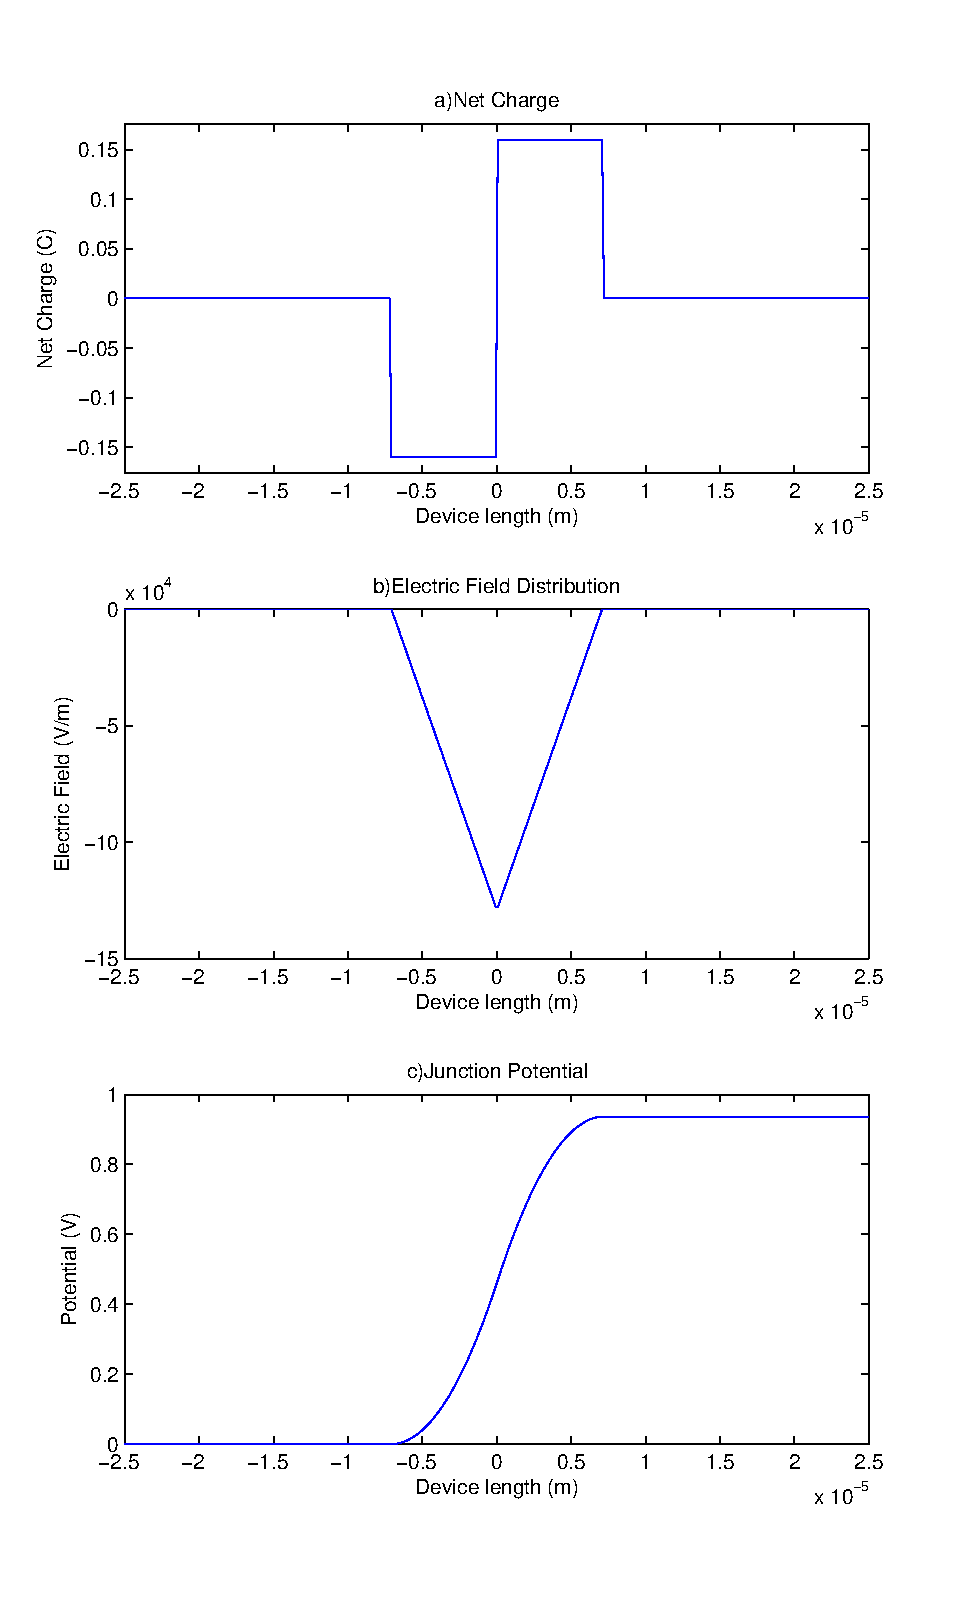
\includegraphics[scale=0.6]{3332}
\caption{Approximate Solution of a PN Junction} 
\label{pnplt}
\end{figure}

\end{doublespace}

 


\chapter{Numerical Solution of Drift-Diffusion Equation} % Main chapter title

\label{Chapter3} % Change X to a consecutive number; for referencing this chapter elsewhere, use \ref{ChapterX}

\lhead{Chapter 3. \emph{Numerical Solution for Drift-Diffusion Equations}} % Change X to a consecutive number; this is for the header on each page - perhaps a shortened title
\begin{doublespace}


As discussed in the introduction, memristor simulations with detailed physical effects are almost non existent. Memristor simulation developed in this thesis requires certain properties ,such as limitation of particle density or combination of 1-D and 2-D simulations, which may not be available in most commercial simulators. It is also possible that other unusual properties that are not studied in this thesis will be needed for further research. In this chapter a method for solving drift diffusion equations as well as Poisson's equation are developed based on finite difference method. This fully functioning simulator will have the needed flexibility for current and future research opportunities.  


\section{Finite Difference Method}
There are many different methods that can be used to solve drift diffusion equations such as finite elements, finite difference or meshless methods. Finite difference was chosen as an appropriate method for this thesis due to its simplicity which allows straightforward implementation of unusual physical properties. Finite difference uses an approximation for the derivative of a function based on the mathematical definition of the derivative\cite{numerical2}.

\begin{equation}
\frac{df}{dx}=\lim\limits_{h \rightarrow 0} \frac{f(x+h)-f(x)}{h}
\end{equation}

It is possible to obtain a numerical approximation for the first derivative of a function by dropping the limit and assuming that h is small enough that the numerical derivative is reasonably close to the actual derivative. As h gets smaller the approximation becomes more and more accurate. The difference between the calculated value and the real value is called the truncation error and it is captured using $O(h^n)$ notation. n signifies the order of h which determines how fast the approximation is approaching the real solution as h decreases.  
\begin{equation}
\frac{df}{dx}=\frac{f(x+h)-f(x)}{h} + O(h)
\label{numdif}
\end{equation}

It is possible to uniformly discretize the entire region over which a function is defined in order to calculate its derivative. The first step is the division of the region over which the function is defined into \textit{n-1} segments. This creates \textit{n} number of points. Then the length of each segment is defined using the following relationship:

\begin{equation}
h=\frac{L}{n}
\end{equation}

A function is defined at the edge of every segment. All the points can be labeled consecutively, $x_0,x_1,x_2$ ... $x_{n-1}$ where $x_i=ih$. The function is discretely defined on \textit{$f_{i}=f(x_{i})$} where\textit{ i=0,1,2..n-1}. It is possible to use equation  \ref{numdif} to discretely calculate the first derivative of the function with respect to x.

\begin{equation}
\frac{df(x_i)}{dx}=\frac{f(x_{i+1})-f(x_i)}{h} + O(h)
\end{equation}
Above equation is called forward difference because the derivative for point $x_i$ was calculated using the point that is coming right after it, $x_{i+1}$.
\begin{equation}
f^{'}_i=\frac{f_{i+1}-f_i}{h}+ O(h)
\end{equation}

Forward difference is not the only way to calculate a numerical derivative. Here are a few other ways calculate the same derivative by using of different points.

\begin{equation}
f^{'}_i=\frac{f_{i}-f_{i-1}}{h}+ O(h)
\label{bdif}
\end{equation}

\begin{equation}
f^{'}_{i+\frac{1}{2}}=\frac{f_{i+1}-f_i}{h}+ O(h^2)
\label{cdif}
\end{equation}

Equation \ref{bdif} is called backward difference and equation \ref{cdif} is called central difference. One important aspect to note here is that in the central difference formula the derivative falls exactly in the middle of two points. It also gives more accurate results using the same number of points as forward and backward difference. 

Using finite difference formulas it is possible to construct higher order derivatives. A formula for a second order derivative at point $x_i$ using central difference can be calculated using a first order derivative on $x_{i-\frac{1}{2}}$, $x_i$ and $x_{i+\frac{1}{2}}$  

\begin{equation}
f_{i+\frac{1}{2}}^{'}=\frac{f_{i+1}-f_{i}}{h}
\label{forwardd}
\end{equation}

\begin{equation}
f_{i-\frac{1}{2}}^{'}=\frac{f_{i}-f_{i-1}}{h}
\label{backwardd}
\end{equation}

\begin{equation}
f^{'}_{i}=\frac{f_{i+\frac{1}{2}}-f_{i-\frac{1}{2}}}{h}
\label{2ndord}
\end{equation}

The second order derivative is constructed by taking the second derivative of the last function. Then equations \ref{forwardd} and \ref{backwardd} are placed into \ref{2ndord}.

\begin{equation}\nonumber
f^{''}_{i}=\frac{f_{i+\frac{1}{2}}^{'}-f_{i-\frac{1}{2}}^{'}}{h}
\end{equation}

\begin{equation}\nonumber
f^{''}_{i}=\frac{\frac{f_{i+1}-f_{i}}{h}-\frac{f_{i}-f_{i-1}}{h}}{h}
\end{equation}

\begin{equation}\nonumber
f^{''}_{i}=\frac{f_{i+1}-f_{i}-f_{i}+f_{i-1}}{h^2}
\end{equation}

Second order derivative takes the following form:

\begin{equation}
f^{''}_{i}=\frac{f_{i+1}-2f_{i}+f_{i-1}}{h^2}+O(h^2)
\label{fdc2}
\end{equation}

Overall these finite difference equations are enough to solve drift diffusion equations. Even though all the derivations are done in 1-D it is trivial to extend them to other dimensions. This method can be used to solve Poisson's equation and drift diffusion equations.

\clearpage

\section{Poisson Solver}

Poisson's equation needs to be solved before drift diffusion equations in order find the potential distribution as well as the electric field inside the device. In order to solve for the electric field and the potential, Poisson's equation is simplified through assumptions and then finite difference method is used to solve this simplified equation\cite{smith1985numerical}. The first step of simplification is assuming that the permittivity is isotropic.
 
\begin{equation}
\nabla \cdot  (\varepsilon \nabla V)=-\rho
\end{equation}

\begin{equation}
\nabla \cdot  (\varepsilon \nabla V)=\varepsilon  \nabla^2 V
\end{equation}

Dividing both sides by permittivity and expanding the left hand side,,

\begin{equation}
 \nabla^2 V =-\frac{\rho}{\varepsilon}
 \label{Poissons}
\end{equation}

\begin{equation}
 \nabla^2 V =\frac{\partial^2 V}{\partial^2 x}+\frac{\partial^2 V}{\partial^2 y}
\end{equation}

After discretizing the electric potential over a uniform 2-D grid and using the second order central finite difference formula \eqref{fdc2} laplacian of the electric potential can be calculated using:

\begin{equation}
 \nabla^2 V_{i,j}=\frac{V_{i+1,j}-2V_{i,j}+V_{i-1,j}}{\Delta x^2}+\frac{V_{i,j+1}-2V_{i,j}+V_{i,j-1}}{\Delta y^2}
 \label{nablafd}
\end{equation}

Since the grid is uniform the distance between two nodes in x and y directions are equal therefore only one variable is needed to represent the distance between two points.

\begin{equation}
\Delta=\Delta x =\Delta y
\label{delta}
\end{equation}

Net charge density and the permittivity is also discretized over the same uniform mesh. Discretized form of Poisson's equation is generated by combining equations \ref{Poissons} ,\ref{nablafd} and \ref{delta}.

\begin{equation}
 \nabla^2 V_{i,j}=\frac{V_{i-1,j}+V_{i,j-1}-4V_{i,j}+V_{i+1,j}+V_{i,j+1}}{\Delta^2}=-\frac{\rho_{i,j}}{\varepsilon_{i,j}}
\end{equation}

This equation can be rearranged into the form below:
\begin{equation}
\varepsilon_{i,j}(V_{i-1,j}+V_{i,j-1}-4V_{i,j}+V_{i+1,j}+V_{i,j+1})=-\Delta^2\rho_{i,j}
\label{discrete_poisson}
\end{equation}

Equation \ref{discrete_poisson} is valid for almost all the nodes in the system except two cases, boundary nodes and interface nodes. There are two different types of boundary conditions. The first one is Dirichlet boundary condition which forces a particular value for the potential at the boundary.

\begin{equation}
V_{i,j}=V_{b}
\label{dirichlet}
\end{equation}

Where $V_{b}$ is the value of the potential at the boundary. The other possible boundary condition is called Neumann boundary condition which states that the derivative of the potential at the boundary is zero. This gives the following equation:

\begin{equation}
\frac{\partial V}{\partial x}=\frac{V_{i+1,j}-V_{i,j}}{\Delta}=0
\label{neumannx}
\end{equation}

So for a boundary in y direction:

\begin{equation}
V_{i+1,j}=V_{i,j}
\label{neumanny}
\end{equation}

Neumann boundary condition in x direction is obtained by using the same procedure.

\begin{equation}
V_{i,j+1}=V_{i,j}
\end{equation}

Combining the equations above (\ref{discrete_poisson}, \ref{dirichlet},\ref{neumannx} and \ref{neumanny}) it is possible to turn Poisson's equation, which is a second order differential equation, into a linear set of coupled algebraic equation.

\begin{equation}
D_{2}\vec{V}=-\Delta^2\vec{\rho}-\vec{V_b}
\end{equation}

$D_{2}$ is the Laplace operator converted into a matrix using the finite difference method. One can easily get the potential distribution by simply solving this matrix equation. Due to the nature of the problem the resulting matrix is quite sparse and using a sparse LU rather than a regular LU decomposition increases the computational efficiency. Additionally, LU decomposition only needs to be performed once since the equation is static and L and U matrices can be reused for all the solutions following the initial one. 

\begin{equation}
\vec{V}=D_{2}^{-1}(-\Delta^2\vec{\rho_{i,j}}-\vec{V_b})
\end{equation}

After solving for the potential distribution it is straightforward to calculate the electric field distribution discretely by using the relationship between the electric field and the electric potential \eqref{Efield} and the central difference equation \eqref{cdif}. 

\begin{equation}
\vec{E^x_{i,j}}=-\frac{V_{i+1,j}-V_{i-1,j}}{2\Delta}
\end{equation}

\begin{equation}
\vec{E^x_{i,j}}=-\frac{V_{i,j+1}-V_{i,j-1}}{2\Delta}
\end{equation}

\clearpage
\section{Current Density Equations}
 Both drift and diffusion currents can be calculated over the entire grid. Drift current does not involve any differentials but it is a function of the electric field and the diffusion current can be calculated using first order central difference\cite{Dragica1}. The current density is calculated in such a way that it falls between two points which simplifies the application of the boundary conditions.
\begin{equation}
J^x_{i+\frac{1}{2},j,k}=q\mu_n n_{i+\frac{1}{2},j,k} E^x_{i+\frac{1}{2},j,k}+D_n \frac{n_{i+1,j,k}-n_{i,j,k}}{\Delta}
\end{equation}
The electric field is calculated exactly on the nodes and linear interpolation is used in order to get a value between the nodes. The same argument is also valid for particle densities \textit{p} and \textit{n}. They are defined at the nodes but they are linearly interpolated to be used in current density equations.

\begin{equation}\nonumber
n_{i+\frac{1}{2},j,k}=\frac{n_{i+1,j,k}+n_{i,j,k}}{2}
\end{equation}
\begin{equation}\nonumber
E^{x}_{i+\frac{1}{2},j,k}=\frac{E^y_{i+1,j,k}+E^y_{i,j,k}}{2}
\end{equation}

Current density in y direction is calculated by following the same method:

\begin{equation}
J^y_{i,j+\frac{1}{2},k}=q\mu_n n_{i,j+\frac{1}{2},k} E^y_{i,j+\frac{1}{2},k}+D_n \frac{n_{i,j+1,k}-n_{i,j,k}}{\Delta}
\end{equation}
\begin{equation}\nonumber
n_{i,j+\frac{1}{2},k}=\frac{n_{i,j+1,k}+n_{i,j,k}}{2}
\end{equation}
\begin{equation}\nonumber
E^{y}_{i,j+\frac{1}{2},k}=\frac{E^y_{i,j+1,k}+E^y_{i,j,k}}{2}
\end{equation}


\clearpage
\subsection{Continuity Equation}
The continuity equation is needed to calculate a transient solution for the drift diffusion equations. The equation is simple to discretize using the finite difference method. There are two terms that need to be discretized, a first order derivative in time and a first order derivative in space. First the divergence term in the equation \eqref{conn} needs to be evaluated.

\begin{equation}
\nabla \cdot J=\frac{\partial J}{\partial x}+\frac{\partial J}{\partial y}=\frac{d J_x}{d x}+\frac{d J_y}{d y}
\end{equation}

It is possible to replace the derivative with central finite difference terms.
\begin{equation}
\frac{d J_x}{d x}=\frac{J^x_{i+\frac{1}{2},j,k}-J^x_{i-\frac{1}{2},j,k}}{h}
\end{equation}
\begin{equation}
\frac{d J_y}{d y}=\frac{J^y_{i,j+\frac{1}{2},k}-J^y_{i,j-\frac{1}{2},k}}{h}
\end{equation}
\begin{equation}
\nabla \cdot J_{i,j,k}=\frac{J^x_{i+\frac{1}{2},j,k}-J^x_{i-\frac{1}{2},j,k}}{h}+\frac{J^y_{i,j+\frac{1}{2},k}-J^y_{i,j-\frac{1}{2},k}}{h}
\label{delJ}
\end{equation}

This is the general form of the divergence of the current density. These set of equations can be placed into a matrix which is a linear function of particle density at time t.

\begin{equation}
B = \nabla \cdot J_k 
\label{fd_div}
\end{equation}

The time derivative can be replaced by a forward or a backward finite difference term respectively.

\begin{equation}
\frac{\partial  \vec{n}_k}{\partial t}=\frac{ \vec{n}_{k+1}-\vec{n}_k}{\Delta t}
\label{forwardtime}
\end{equation}

\begin{equation}
\frac{\partial \vec{n}_k}{\partial t}=\frac{ \vec{n}_k- \vec{n}_{k-1}}{\Delta t}
\label{backwardtime}
\end{equation}

It is possible to find a numerical transient solution for the drift-diffusion problem by combining finite difference form of the time derivative (\eqref{forwardtime} or \eqref{backwardtime}) and the divergence of the current density equations \eqref{fd_div}.

Forward difference approximation can be used to get an explicit solution for the continuity equation.

\begin{equation}\nonumber
\frac{ \vec{n}_{k+1}-\vec{n_k}}{\Delta t}=B
\end{equation}

\begin{equation}
\vec{n}_{k+1}=\vec{n_{k}}+\Delta t B
\label{explicit}
\end{equation}

Both forward and backward difference formulas work sequentially in order to generate a transient solution. The solution from the previous time step is needed to calculate the solution for the next time step. The forward difference gives an explicit solution which has a few advantages. This solution can be implemented, without forming any matrices by directly calculating the divergence of the current density for each node and then marching through time using equation \ref{explicit}. Additionally, unlike backward difference, there are no equations to be solved for every time step. These two properties ease the computational load of the problem and speed up the solution process. Unfortunately this scheme has very strict stability conditions which have to be met in order to produce a solution.

Backward difference can be replaced by forward difference to get an implicit solution.
\begin{equation}\nonumber
\frac{ \vec{n}_{k}-\vec{n}_{k-1}}{\Delta t}=\frac{1}{q}(qB)
\end{equation}
\begin{equation}\nonumber
\vec{n}_{k}-\Delta t B =\vec{n}_{k-1}
\end{equation}

Since all the equations in B matrix are a linear functions on n, it can be separated into two terms, $B=Cn$.
\begin{equation}\nonumber
\vec{n}_{k}-\Delta t C\vec{n}_{k-1} =\vec{n}_{k-1}
\end{equation}
\begin{equation}
\vec{n}_k=(I-\Delta t C)^{-1}\vec{n}_{k-1}
\end{equation}

This solution needs a matrix inversion every time step but it is unconditionally stable if it is not coupled with Poisson's equation. The decision to use an implicit or an explicit solution requires deliberate analysis and it will be discussed in detail in the section following boundary conditions.
\clearpage


\subsection{Boundary Conditions}

For the drift diffusion problem solved in this thesis there are two different possibilities for boundary conditions on mobile charged particles. No flow conditions are imposed on the current density equations where metal contact condition is imposed on the particle densities. There are two sub types of no flow boundary conditions used during simulation,a regular and a dependent no flow boundary condition. A regular no flow condition is used when the particles cannot go past a certain boundary. This is achieved by setting the particle flow at any boundary to zero. 

Dependent no flow boundary condition is a term that is used to describe a boundary condition which can be a function of any variable such as temperature, particle or charge density. For the lithium ions this condition is a function of lithium density and it is used not only for the boundaries but also for all the points inside the PEDOT:PSS. During simulation, at any point inside PEDOT:PSS if the lithium density reaches a certain limit then that point turns into a no flow wall for the lithium ions as long as there is a net influx of particles. The boundary condition is removed if the lithium density at that point will go below the set limit at the next time step during transient simulation.  

To simulate the metal contacts it is assumed that they hold an infinite amount of positive and negative charges and the boundary is always charge neutral. For example for holes, electrons, positive and negative doping it is assumed that at the boundary positive charge concentration will be equal to the negative charge concentration. 

\begin{equation}
N_{D} + p=N_{A} + n
\label{chargeneutrality}
\end{equation}

For a semiconductor holes and electrons have to obey the mass action law.

\begin{equation}
np=n_i^2
\label{massaction}
\end{equation}

$n_i$ is the concentration of the semiconductor at equilibrium before getting doped. Solving \eqref{massaction} and \eqref{chargeneutrality} together results in the equation below:

\begin{equation}
p=\frac{1}{2}(N_A - N_D + \sqrt{(N_A - N_D)^2+4n_i^2})
\label{nbound}
\end{equation}

Once the hole concentration is obtained it is possible to calculate the electron concentration using the mass action law.

\begin{equation}
n=\frac{n_i^2}{p}
\label{pbound}
\end{equation}

Figures \ref{bc_hole}, \ref{bc_lithium} and \ref{bc_perchlorate} show the boundary conditions used for holes, lithium and perchlorate ions.

\begin{figure}[!htp]
\centering
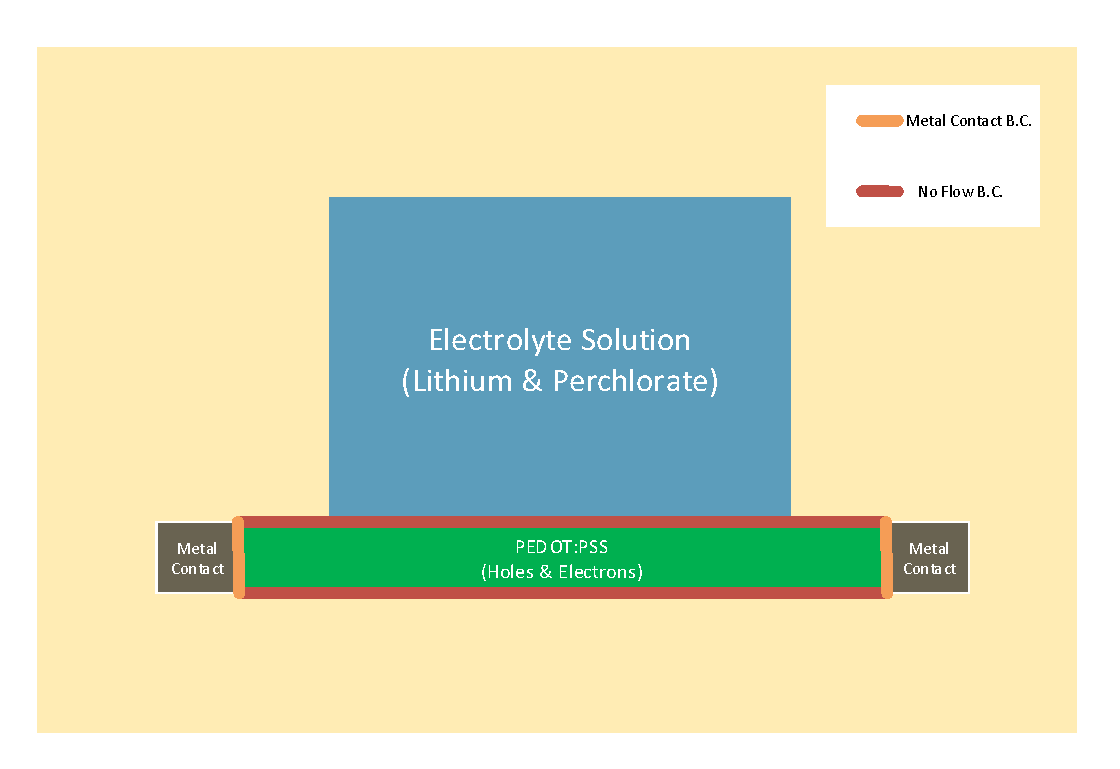
\includegraphics[scale=0.6]{bc_hole}
\caption{Boundary conditions for the holes } 
\label{bc_hole}
\end{figure}

\begin{figure}[!htp]
\centering
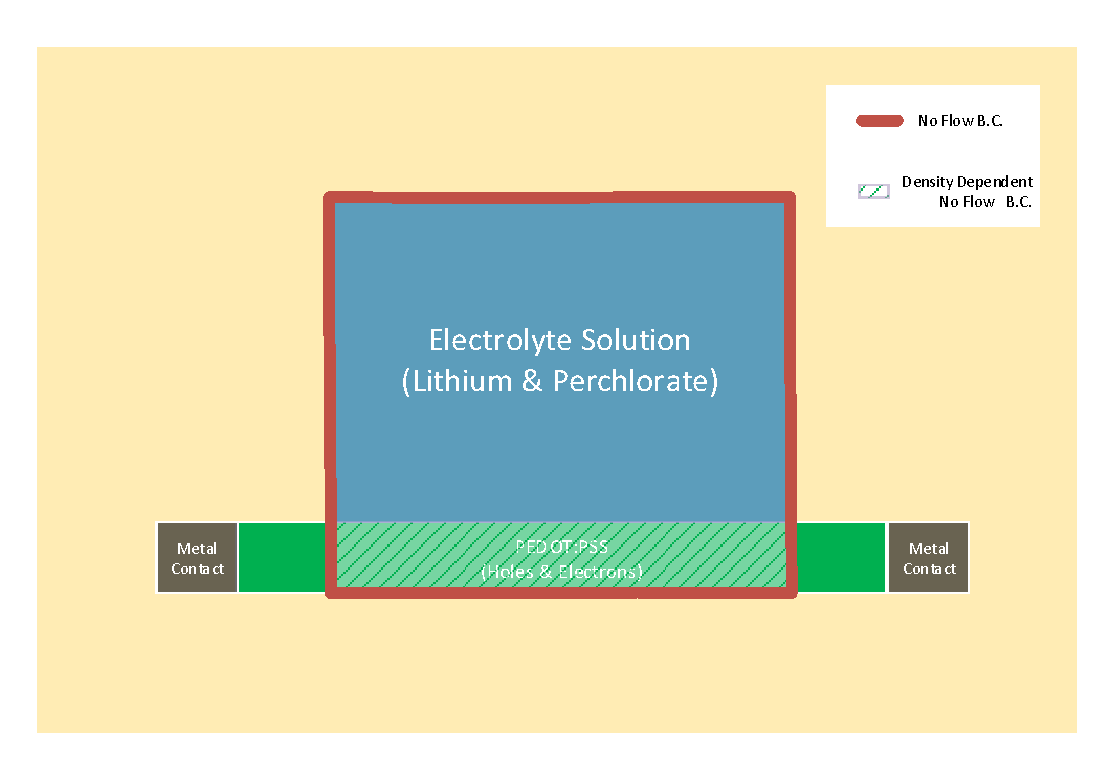
\includegraphics[scale=0.6]{bc_lithium}
\caption{Boundary conditions for the lithium ions } 
\label{bc_lithium}
\end{figure}

\begin{figure}[!htp]
\centering
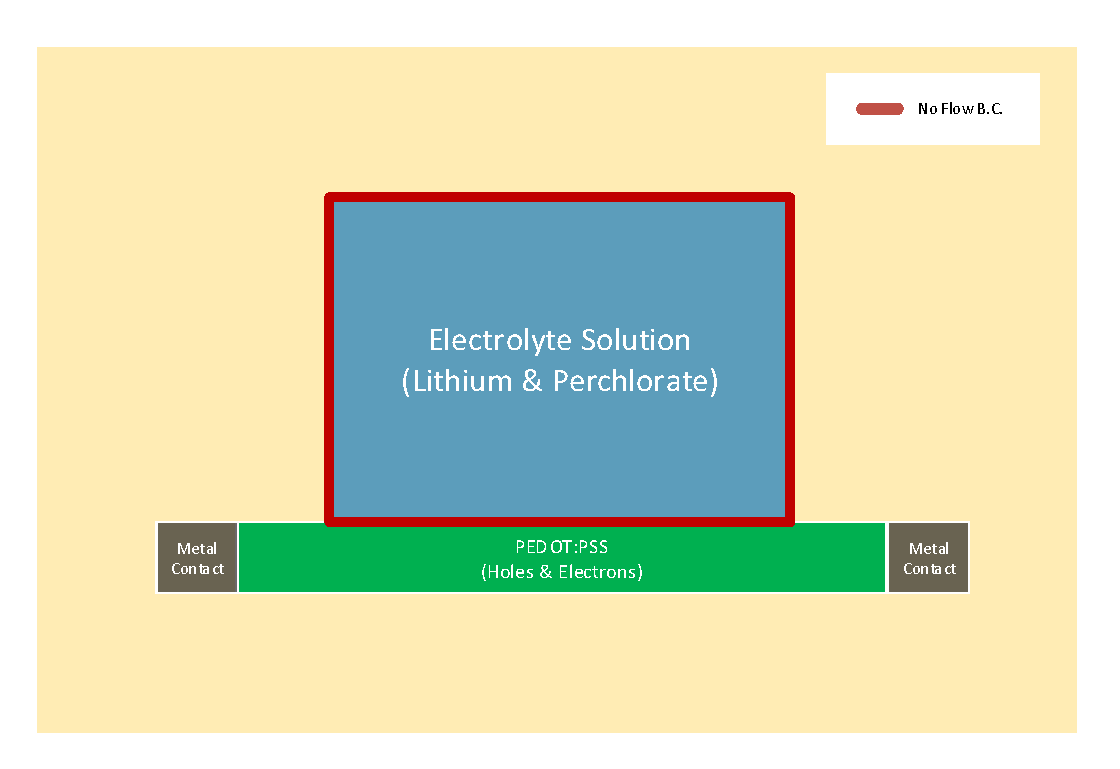
\includegraphics[scale=0.6]{bc_perchlorate}
\caption{Boundary conditions for the perchlorate ions } 
\label{bc_perchlorate}
\end{figure}

During simulation, the application of the metal contact boundary condition differs from the no flow boundary which is applied implicitly. All the boundaries are simulated using a no flow condition by default but for metal contacts boundary values are set to the appropriate values at the end of every time step. The lack of charge is compensated and excess charge is taken off by the metal contact. The difference between the boundary value of the charge density and its actual value is used to calculate the derivative of the current density with respect to time. The current in and out of the device is calculated by integrating the derivative of the current density over time. 

\begin{equation}
\frac{dn}{dt}=\frac{n_{cr}-n_{ct}}{\Delta t}
\end{equation}

$n_{cr}$ is the excess carrier density and $n_{ct}$ is the equilibrium carrier density at the contact. Using these boundary conditions for holes and electrons and the following two equations it is possible to calculate incoming and outgoing currents. 

\begin{equation}
Q=An
\label{charge_charge_density}
\end{equation} 

\begin{equation}
I=\frac{dQ}{dt}
\label{current_charge}
\end{equation} 
 

Equation \ref{charge_charge_density} is an approximate relationship between charge and charge density where Q is total charge, A is the area holding that charge. Equation \ref{current_charge} is simply the general definition of current. By combining these two equations it is possible to derive a formula for calculating the current leaving or entering the device at any metal contact.

\begin{equation}
I=A \frac{dn}{dt}
\label{current_charge_density}
\end{equation}


\section{Stability and Computational Efficiency}
Before discussing  the numerical limitations of solving the drift diffusion equation via finite difference it is important to look into the physical limitations of the problem. These limitations persist no matter what kind of numerical scheme is employed to solve the drift diffusion equation.

\subsection{Physical Limitations}
Debye length is the length over which mobile charge carriers screen out an external electric field and it determines how steeply charges will accumulate over a certain distance.
\begin{equation}
L_D=\sqrt{\frac{\varepsilon V_{th}}{q n}}
\label{debye}
\end{equation}
Debye length limits how coarse the grid can be since the distribution of the charge density needs to be accurately captured. As it can be seen from the formula above the higher the charge density is the steeper the charge will accumulate. This behavior is also appears in the analytic solution provided in section 2.2.1 in chapter 2. The accumulation of the charged particle at the wall becomes steeper as the electric field strength increases. The debye length can become a major problem for large devices with high charge densities since the mesh density needs to be extremely high.

The amount of time it takes for charge fluctuations to disappear is called Dielectric relaxation time. It limits the maximum time step of a simulation since the fluctuations that are not properly resolved over time will make the simulation unstable.

\begin{equation}
t_{dr}=\frac{\varepsilon}{q n \mu}
\label{tdr}
\end{equation}

Dielectric relaxation time is only important when the electric potential is highly affected by the redistribution of charge over time. Otherwise it has minimal impact on the stability of the problem.
\subsection{Numerical Limitations}

There are also numerical limits which can affect convergence and stability of a solution when using an explicit finite difference scheme. These are called Courant-Friedrichs-Lewy (CFL)conditions \cite{NumModel}. CFL conditions for diffusion and drift are shown in the following equations.

\begin{equation}
\frac{\Delta ^2}{2 D_n}>\Delta t
\label{CFL_Diff}
\end{equation}

Above condition is for only diffusion and it restricts the maximum time step. Following condition is for drift dominated systems:

\begin{equation}
\frac{2 \Delta }{\mu E}>\Delta t
\label{CFL_Drift}
\end{equation}

This is the second numerical restriction on the simulation. The condition for drift depends on the electric field therefore it needs to be satisfied at all times as the electric field changes over time during simulation.

Both physical and numerical constraints have to be evaluated and mesh density and time step need to be selected in order to satisfy all these conditions discussed above. Particularly mesh density has a very strong impact on the accuracy, stability and the computational efficiency of the simulation. Increasing the mesh density increases the computational time needed to calculate every time step since there are more operations to be performed. Additionally because of the CFL condition for diffusion, time step is related to the square of the mesh size. This means that maximum allowed step size decreases much quicker than the mesh density. Also, increasing charge density can decrease the maximum mesh size to a very small value. This can be fixed by using a non uniform mesh which can dramatically decrease the number points needed for the simulation. This is usually not very straightforward to implement in a finite difference scheme and a small mesh size requires small time steps. This cannot be avoided through non uniform meshing. Both numerical and physical constraints for the memristor simulation are further discussed in chapter 5.

\subsection{Explicit vs. Implicit Solution}

Overall explicit and implicit solutions have their advantages and disadvantages. Choosing one over the other requires a careful analysis of the problem. Implicit solution by itself is unconditionally stable therefore it can support very large time steps without any stability issues. However, the accuracy of the transient solution decreases with a larger time step but the steady state solution does not get affected. So for steady state solutions it is better to use an implicit method which can reach steady state very quickly. This advantage disappears when the particle densities are high enough to affect the electric field and Poisson's equation needs to be solved for every time step. In this scenario the maximum time step is determined by the dielectric relaxation time which can be around the same order as CFL conditions or even smaller. Since the time step is going to be around the same order for both implicit and explicit methods it is reasonable to use the explicit solution because it is computationally less expensive.

Usually an implicit solution is preferable when there is no coupling between Poisson's equation and the drift diffusion equations and the transient response is not very important. Explicit solution has an edge over the implicit solution due to its lower computational requirements when the equations are coupled and the time steps for both schemes are restricted to small values. For memirstor simulation, the drift diffusion equations are strongly coupled with Poisson's equation. For this reason all the memristor simulations in this thesis use explicit time stepping. 


\clearpage
\section{Simulation Procedure}
Different equations and schemes that are used to solve the drift diffusion and Poisson's equation is shown over the past few sections. Using all this information it is possible create a general approach to solve a drift diffusion problem. Following equations are used to simulate the ion and hole movement and the changes in electric field in an organic memristor using finite difference method:

\begin{equation}
\nabla \cdot  (\varepsilon \nabla V)=-q(p-n+N_{D}^{+}-N_{A}^{-})
\end{equation}
\begin{equation}
\vec{J_p}=q\mu_p p \vec{E}-q D_p \nabla p
\end{equation}
\begin{equation}
\vec{J_{N_{A}^{-}}}=q\mu_{N_{A}^{-}} N_{A}^{-} \vec{E}+q D_{N_{A}^{-}} \nabla N_{A}^{-}
\end{equation}
\begin{equation}
\vec{J_{N_{D}^{+}}}=q\mu_{N_{D}^{+}} N_{D}^{+} \vec{E}-q D_{N_{D}^{+}} \nabla N_{D}^{+}
\end{equation}
\begin{equation}
\frac{\partial p}{\partial t}=-\frac{1}{q}\nabla \cdot \vec{J_p}
\end{equation}
\begin{equation}
\frac{\partial N_{A}^{-}}{\partial t}=\frac{1}{q}\nabla \cdot \vec{J_{N_{A}^{-}}}
\end{equation}
\begin{equation}
\frac{\partial N_{D}^{+}}{\partial t}=-\frac{1}{q}\nabla \cdot \vec{J_{N_{D}^{+}}}
\end{equation}

The geometry and the physical properties of the problem as well as all the initial and the boundary conditions need to be defined at the beginning of the solution process. The initialization sets up the first time step of the problem at $t=0$. Once this first step is done it is possible generate the required vectors and matrices and solve the problem for the next time steps, $t=t_i$. 

The solution process starts by solving Poisson's equation using the charge distribution at current time step. Once it is solved, the electric field distribution is calculated and used in the drift diffusion equations to calculate the current density distribution. Explicit time stepping is used to determine the carrier density in the next time step. Finally once the carrier distribution for the next step is calculated it is possible check for a stopping criterion. If this criterion is not met then the whole process will start all over again. If the charge concentration is so small that the equations are decoupled then it is possible to skip solving Poisson's equation for the rest of the simulation which speeds up the solution process.

 There are two different criteria that can be used to decide whether to finalize the simulation process or not. The simulation can stop if it reaches a certain point in time. This is quite simple since the current time can be checked and if it is equal or greater than the required simulation time then the simulation can be stopped. It is also possible to simulate until the simulation reaches steady state. This can be determined by comparing the current carrier distributions with distribution at the previous time step. If the difference is very small then the time derivatives of the carrier densities are very close to zero and the simulation has reached steady state therefore the simulation process can be stopped. The flowchart in figure \ref{flowchart} summarizes the solution procedure.

\clearpage

\begin{figure}
\centering
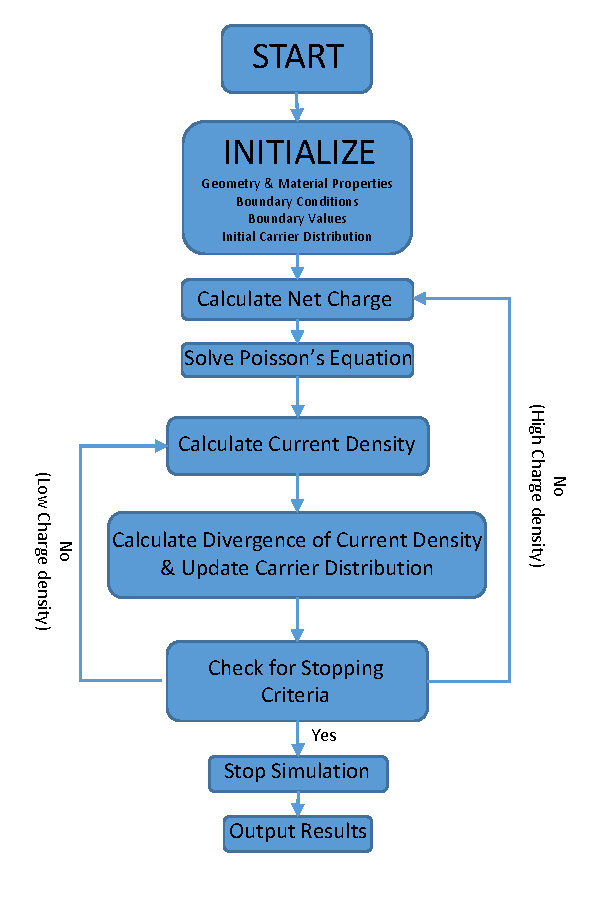
\includegraphics[scale=1.3]{flowchart}
\caption{Finite Difference Drift-Diffusion Scheme Flowchart} 
\label{flowchart}
\end{figure}

\end{doublespace}

% Chapter Template

\chapter{Test Cases: Analytic vs. Numerical Solutions} % Main chapter title

\label{Chapter4} % Change X to a consecutive number; for referencing this chapter elsewhere, use \ref{ChapterX}

\lhead{Chapter 4. \emph{Test Cases: Analytic vs. Numerical Solutions}} % Change X to a consecutive number; this is for the header on each page - perhaps a shortened title

In the past chapter we have gone through the details of how to solve drift-diffusion and Poisson's equation using finite difference method. Now we can do steady state and transient analysis and compare the results with analytical solutions as well as a commercially available simulator called 'COMSOL Multiphysics' which uses finite element method instead of finite difference. Following test cases were made to ensure that the key parts of the finite difference scheme runs properly and does not produce unexpected results. 

\section{Solution for Closed Boundary}
In this test case we will examine the accuracy of the finite difference solution in steady state. In order to do this we can use a simple 1-D problem where we have a finite number of negatively charged particles over a certain distance subject to constant electric field. This is the same problem we have solved analytically in section 3.3.1. We also assume that the charge density is very low and does not affect the electric field. Both ends of the simulation domain have no flow boundary conditions for charged particles. The solution process requires an initial distribution for charge density over the area. For this problem the density of the negative particles was initialized to be uniform over the entire area. Since our differential equations are uncoupled solving Poisson's equation only once is sufficient to determine the electric field over the course of the entire simulation. Figures \ref{5E} and \ref{5pot} show the potential and the electric field distribution over the entire simulation area calculated from Poisson's equation using finite difference. 

\begin{figure}
\centering
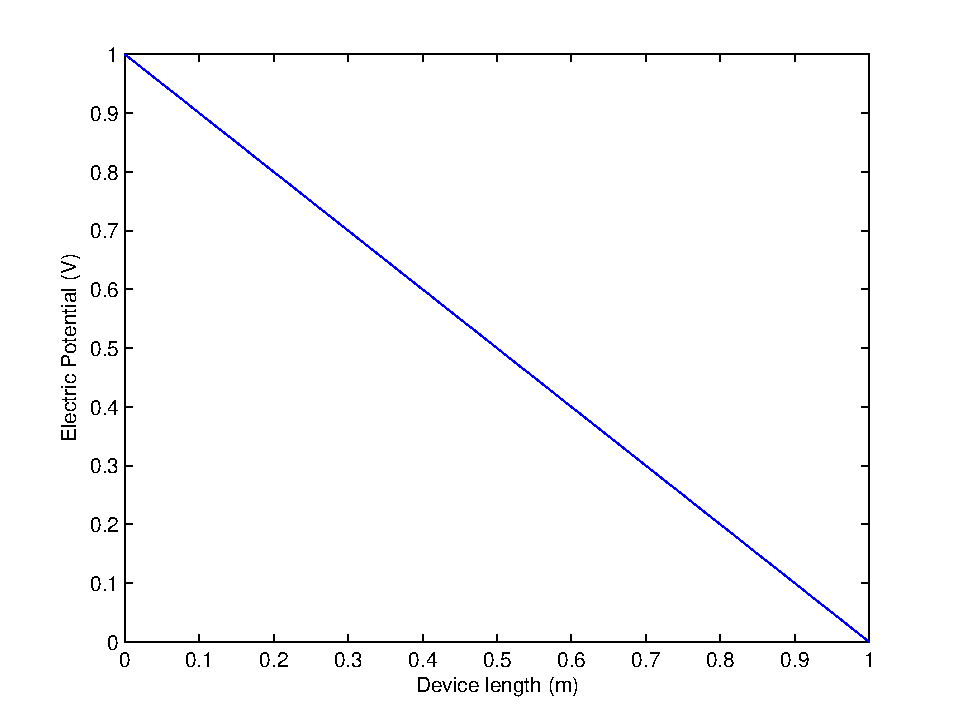
\includegraphics[scale=0.8]{5101}
\caption{Potential Distribution} 
\label{5pot}
\end{figure}

\begin{figure}
\centering
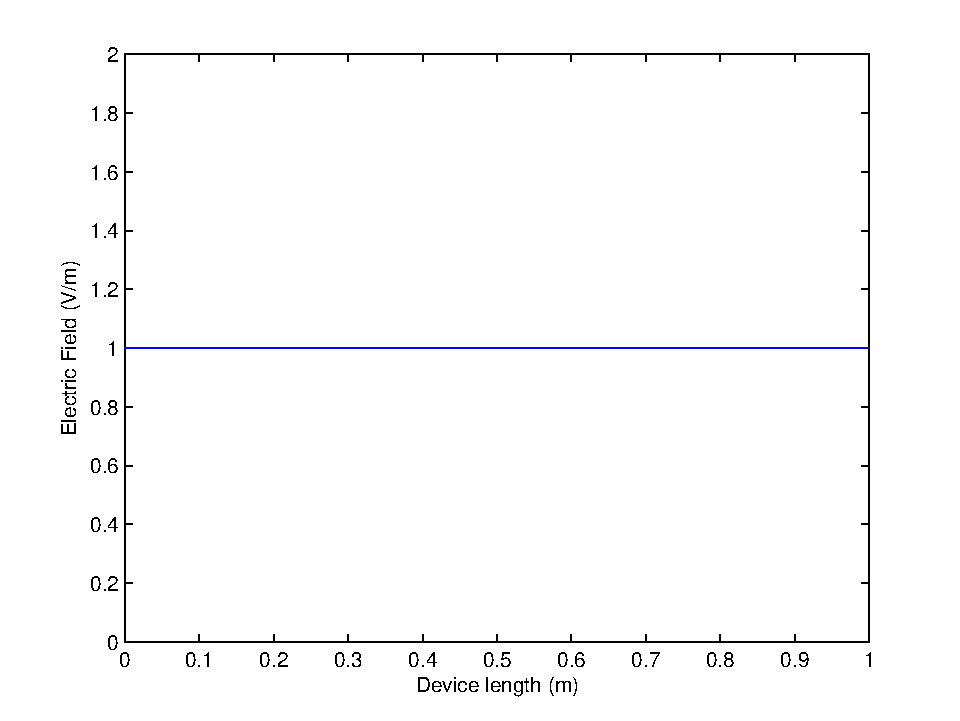
\includegraphics[scale=0.8]{5102}
\caption{Electric Field Distribution} 
\label{5E}
\end{figure}

\clearpage

Figure  \ref{5ss} has two simulation results as well as the exact solution of this problem. The green line represents the result given by the finite difference method once the transient response reaches steady state. It can be seen from the graph that the steady state solution generated by both COMSOL and finite difference matched the analytical solution.

\begin{figure}
\centering
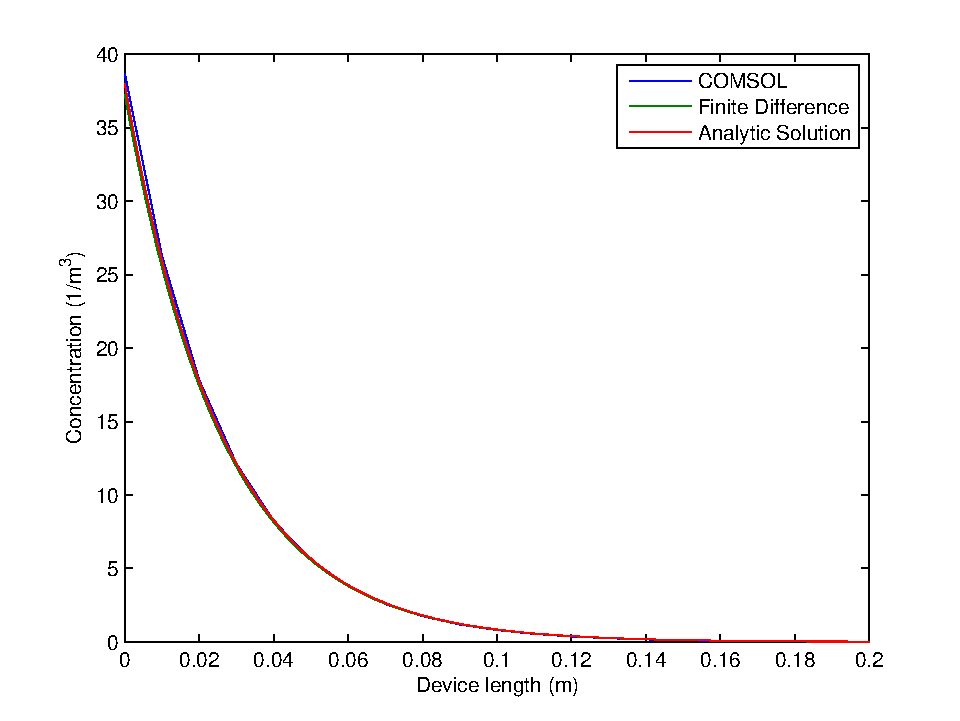
\includegraphics[scale=0.8]{511}
\caption{Steady State Negative Charge Density} 
\label{5ss}
\end{figure}

\begin{figure}[!htp]
\centering
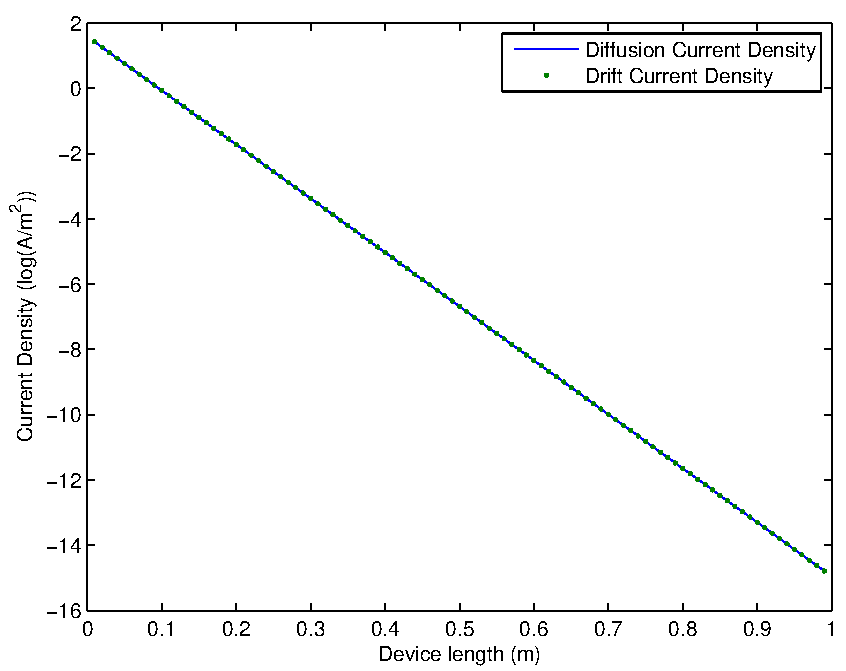
\includegraphics[scale=0.8]{513}
\caption{Finite Difference Drift and Diffusion Current Densities}
 \label{5curdens}
\end{figure}

While deriving an analytical solution for this problem we have assumed that at steady state the drift current density must be equal to the diffusion current density. In figure \ref{5curdens} we see drift and diffusion current densities in log scale. Overall both currents match quite tightly.

\clearpage
\section{Solutions for Open Boundary}
Another very important aspect of drift-diffusion simulation is its transient response. Like the previous test case, we can use a closed form solution to test the accuracy of the transient response. In section 3.3.2 we have found two different analytic solutions for a similar drift diffusion problems which involved infinite boundaries and a uniform electric field. The only difference between two cases are their initial carrier distribution. One has a rectangular and the other one has a gaussian  initial carrier distribution. Since we have not implemented any way to deal with infinite boundaries we will just simulate these two problems until the carrier distributions gets close to one boundary.  

\begin{figure}[ht]
\centering
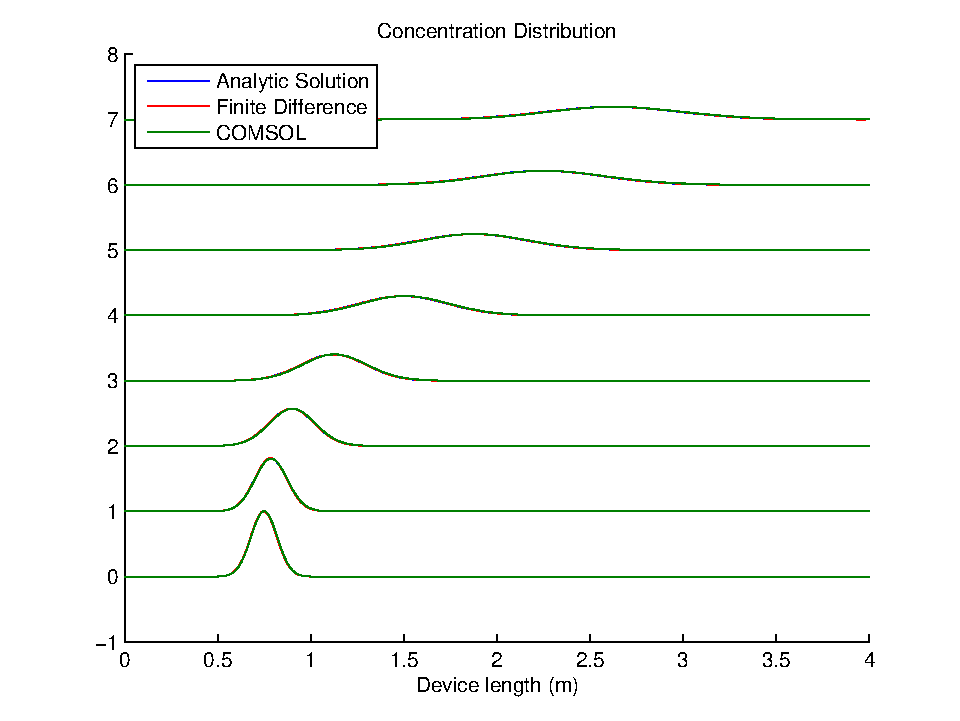
\includegraphics[scale=0.8]{5212}
\caption{Gaussian Carrier Distribution Evolving Over time} 
\label{51}
\end{figure}

Figure \ref{51} has the transient response from COMSOL, finite difference and analytical solution. Snapshots of the carrier distributions were taken for each method at different time steps and they were superposed on top of each other. Increasing levels on y axis represent a carrier distributions at a different time starting from the bottom and moving forward in time towards the top. Figure \ref{51} has a gaussian initial carrier distribution. It can be seen from that the transient solution generated by both COMSOL and finite difference are quite close to the analytical solution.

\clearpage
\section{Hybrid Method}

While developing a method for numerically calculating current density we have seen that Scharfatter-Gummel scheme turns into a first order upwind scheme for drift dominant problems. Most of the time first order upwind schemes has a major drawback which is numerical dispersion. This means that we will see diffusion due to numerical error even though it almost does not exist. In order to investigate this issue and look for possible remedies we will use the previous example ,with a much higher electric field, as a starting point  Here in figure \ref{53} we see the transient response of a drift dominant problem. Finite difference has no problem producing an accurate transient response but SG has a fair amount of numerical diffusion.  

\begin{figure}[ht]
\centering
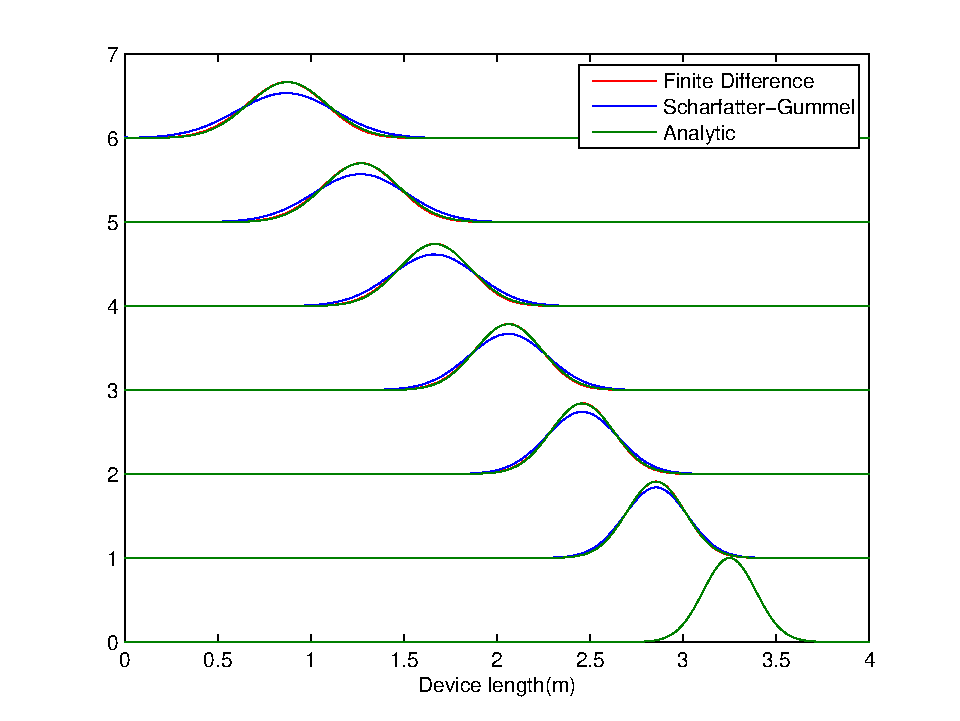
\includegraphics[scale=0.75]{5231}
\caption{Gaussian Carrier Distribution Evolving Over time} 
\label{53}
\end{figure}

We can also look at the differences between finite difference and SG in steady state. In this case as it can be seen from figures \ref{54} and \ref{55} SG produces a solution much closer to the analytical solution. This is not surprising. Both steady state solution and SG scheme has an exponential form. So SG can capture the non-linearity at the boundary much better than finite difference which has linear terms. Also in figure \ref{55} we can see finite difference producing negative carrier density distribution which is not physical and it can easily make the simulation unstable.  


\begin{figure}[!htp]
\centering
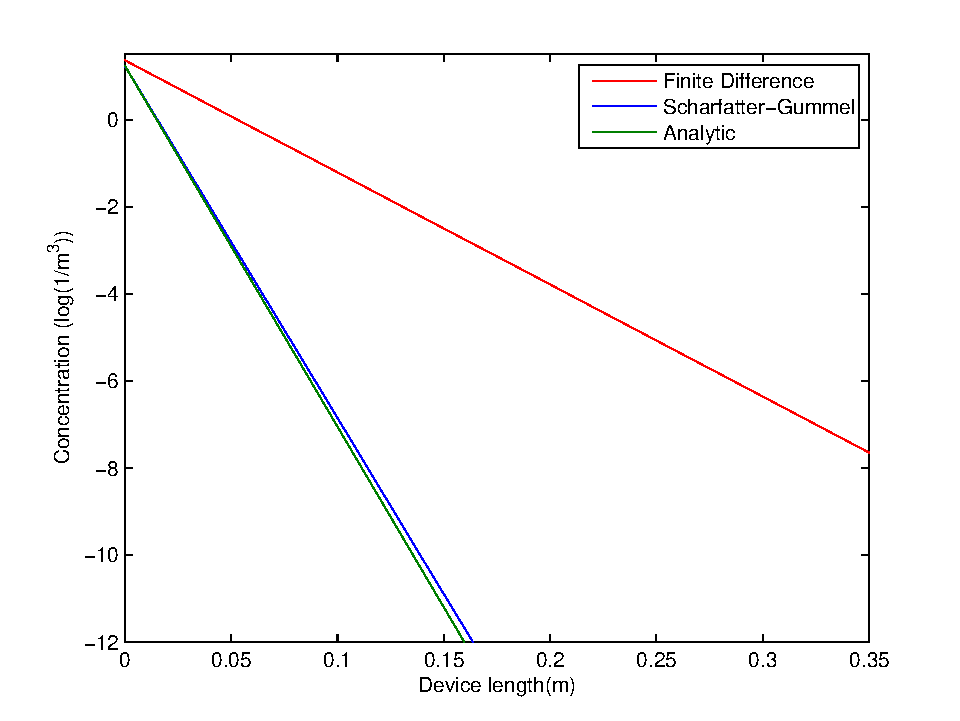
\includegraphics[scale=0.75]{5232}
\caption{Steady State Carrier Distribution of a Drift Dominant Problem} 
\label{54}
\end{figure}

\begin{figure}[!htp]
\centering
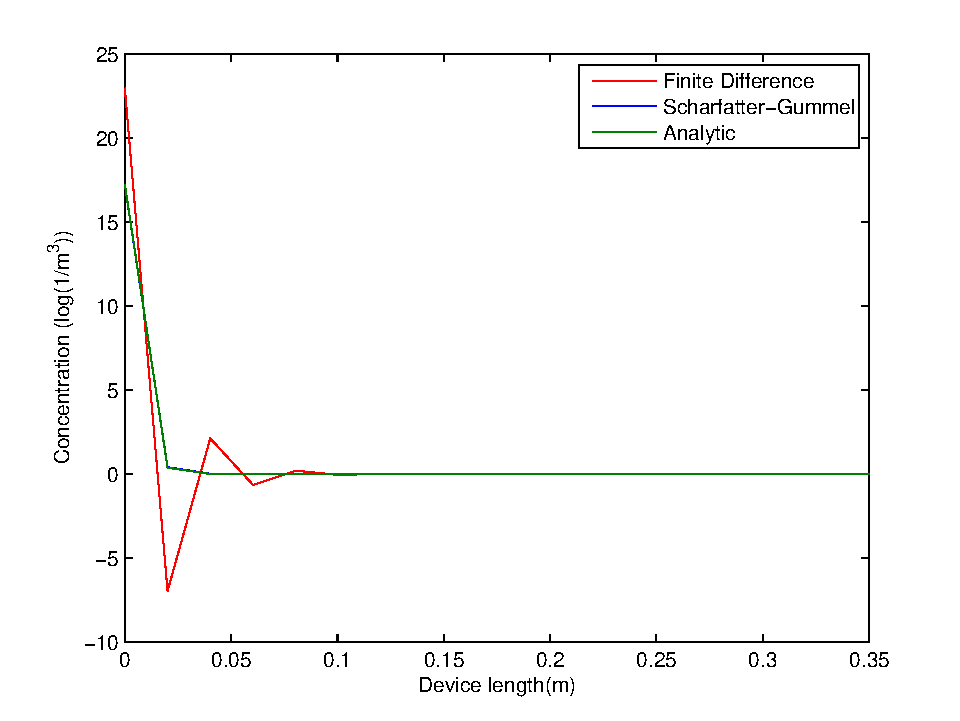
\includegraphics[scale=0.75]{5233}
\caption{Steady State Carrier Distribution of a Drift Dominant Problem} 
\label{55}
\end{figure}

We can see that both methods have their advantages. It is possible to develop a method where we can switch between two methods to get more accurate results. From the analysis above it seems like in transient cases finite difference method have an advantage and SG is better in steady state where drift and diffusion cancel each other out. We can switch between methods by keeping track of two key properties, closeness to steady state and the non linearity of the final solution. The difference between drift and diffusion currents is a good estimator for closeness to steady state and the ratio of drift velocity to diffusion constant can be used to measure non linearity. We can use following two equations to calculate these parameters.

\begin{equation}
K_1=|\frac{J_{drift}+J_{diff}}{J_{drift}-J_{diff}}|
\end{equation}

\begin{equation}
K_2=\frac{\mu E}{D}=\frac{v}{D}
\end{equation}

$K_1$ will always have a value between 0 and 1 depending on how close drift and diffusion current densities are to each other. When $K_1$ is close to 1 it means that drift and diffusion do not have equal values and opposite signs therefore the simulation is far away from steady state. On the other hand if $K_1$ is close to 0 it means that the simulation is in steady state or close to it.  

$K_2$ is a measure of how non linear the solution is going to be since it appears in an exponential. If this value is between 0 and 2 then the final solution is slightly non linear. As $K_2$ increases further the non linearity becomes stronger.

Now that we have established a way to check closeness to steady state and non linearity of the final solution we can use these to improve the accuracy of our transient and steady state responses. During simulation if $K_1$ is close to 1 it means that we are not close to steady state therefore it is better to use finite difference. When $K_1$ is getting close to zero it is time to check if the final solution is going to be very non linear using $K_2$. If that is the case then we can switch to SG method to calculate the steady state solution. Figure \ref{56} shows the evolution of the transient response over time using this hybrid method. The solution is in transient mode so finite difference is used to calculate the current density. As expected numerical diffusion does not occur and the response is quite close to the analytic solution.

Figures \ref{57} to \ref{60} shows the changes in the concentration over time as the simulation approaches steady state. By looking at the following sequence of figures we can see that finite difference has fluctuation problems and it gets worse over time. At the same time we can see the hybrid method transitioning from finite difference to SG method and not having any fluctuation problems. Finally in steady state plots in figure \ref{61} shows the difference in accuracy at steady state between the hybrid method and finite difference. By mixing two methods we were able to reach higher accuracy without needing to increase the mesh density.

\begin{figure}[ht]
\centering
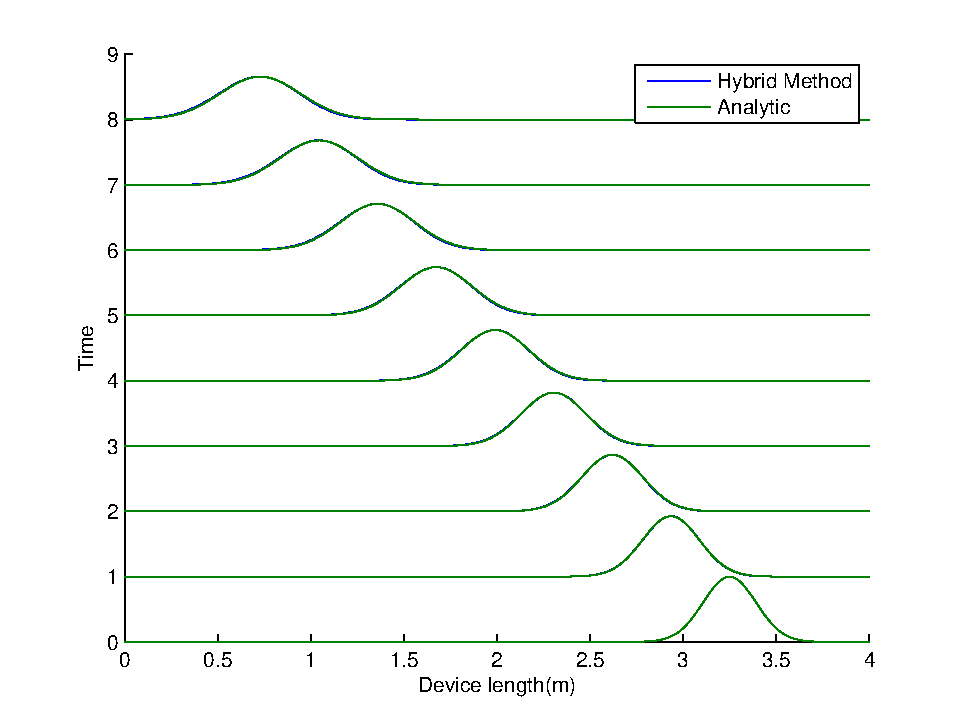
\includegraphics[scale=0.75]{5234}
\caption{Gaussian Carrier Distribution Evolving Over time} 
\label{56}
\end{figure}

\begin{figure}[ht]
\centering
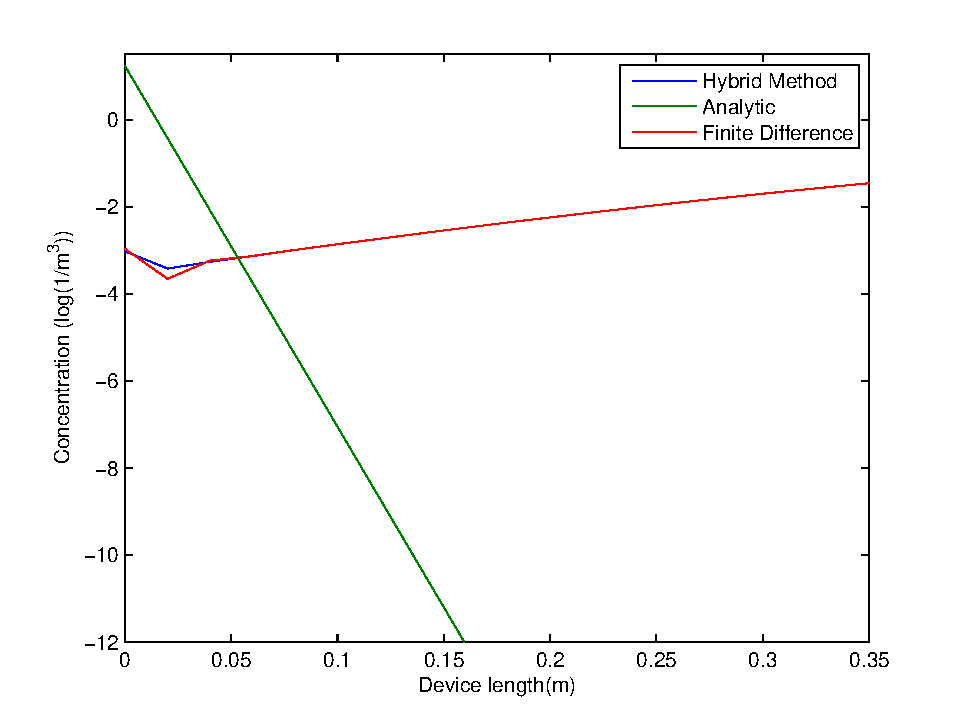
\includegraphics[scale=0.75]{5235}
\caption{Transient Solution of a Drift Dominant Problem} 
\label{57}
\end{figure}

\begin{figure}[ht]
\centering
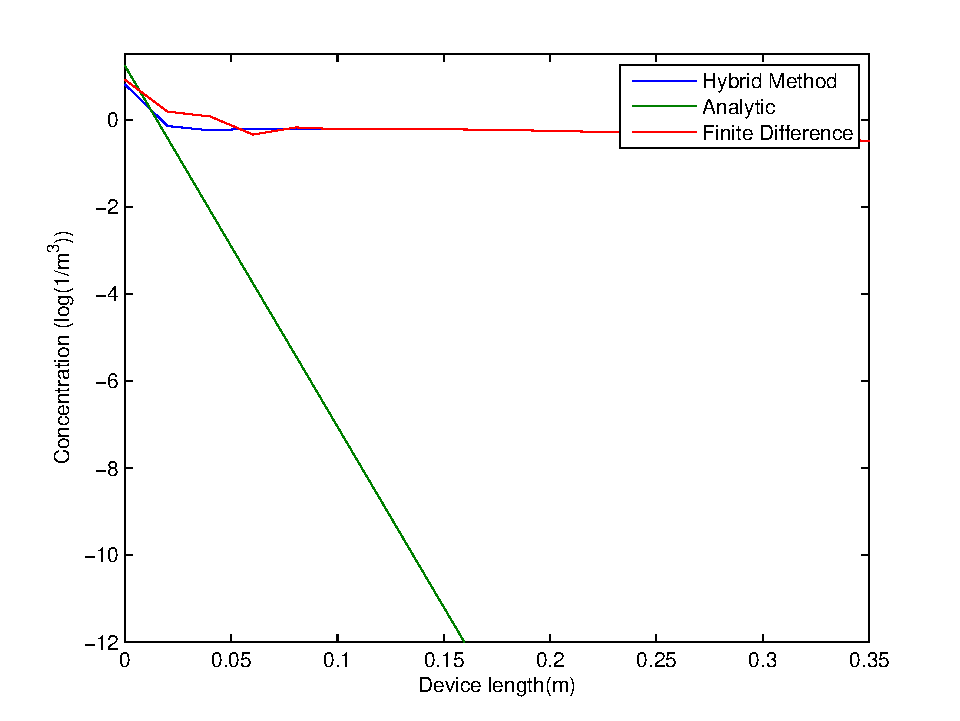
\includegraphics[scale=0.75]{5236}
\caption{Transient Solution of a Drift Dominant Problem} 
\label{58}
\end{figure}

\begin{figure}[ht]
\centering
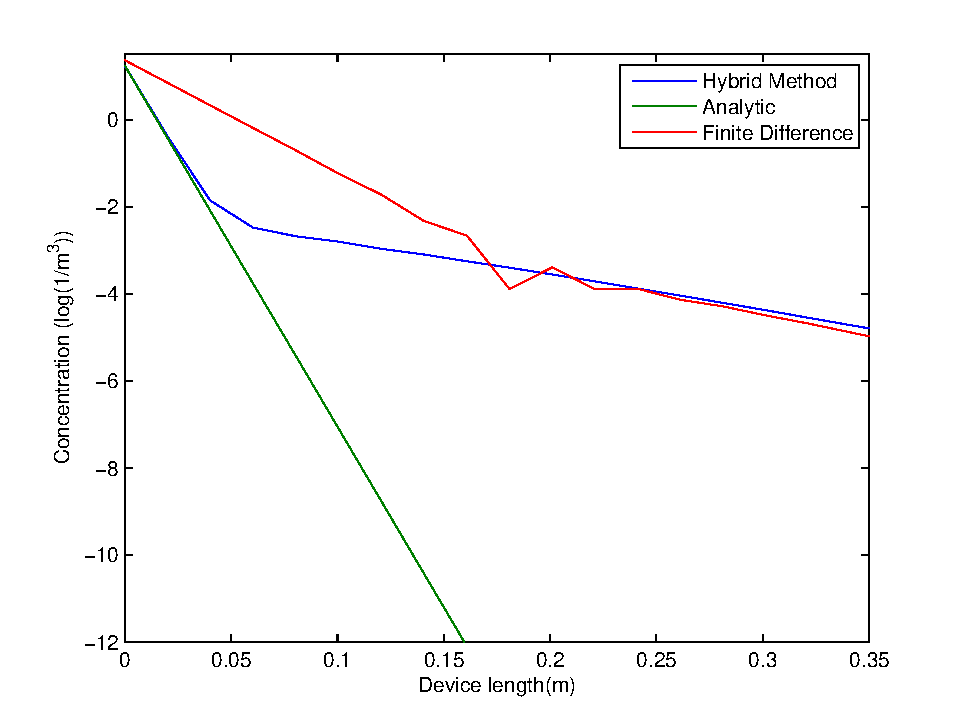
\includegraphics[scale=0.75]{5237}
\caption{Transient Solution of a Drift Dominant Problem } 
\label{59}
\end{figure}

\begin{figure}[ht]
\centering
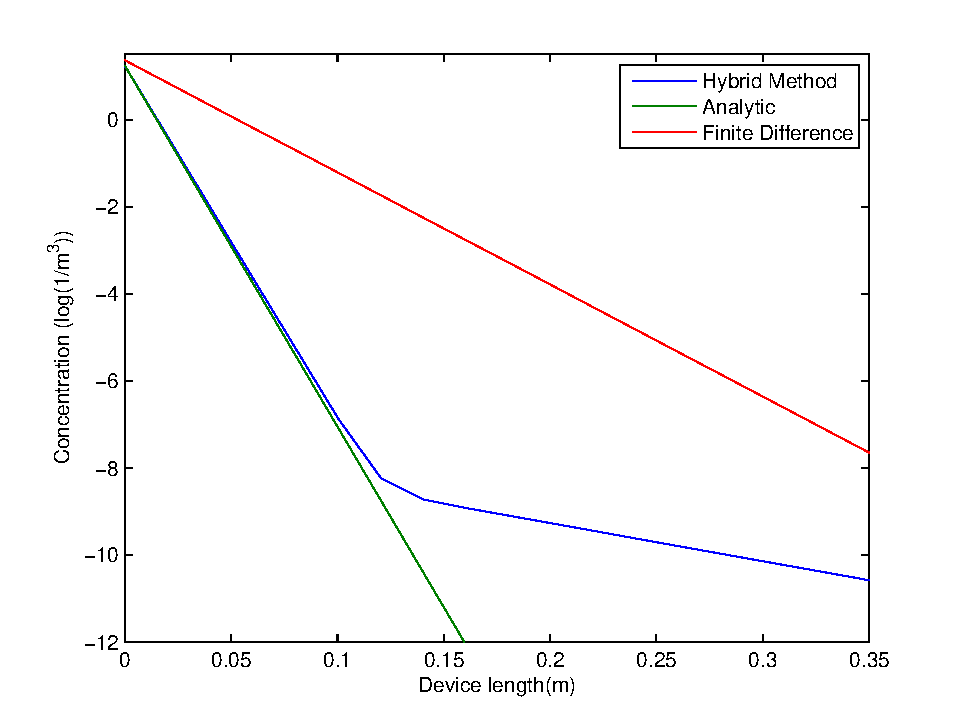
\includegraphics[scale=0.75]{5238}
\caption{Transient Solution of a Drift Dominant Problem } 
\label{60}
\end{figure}

\begin{figure}[ht]
\centering
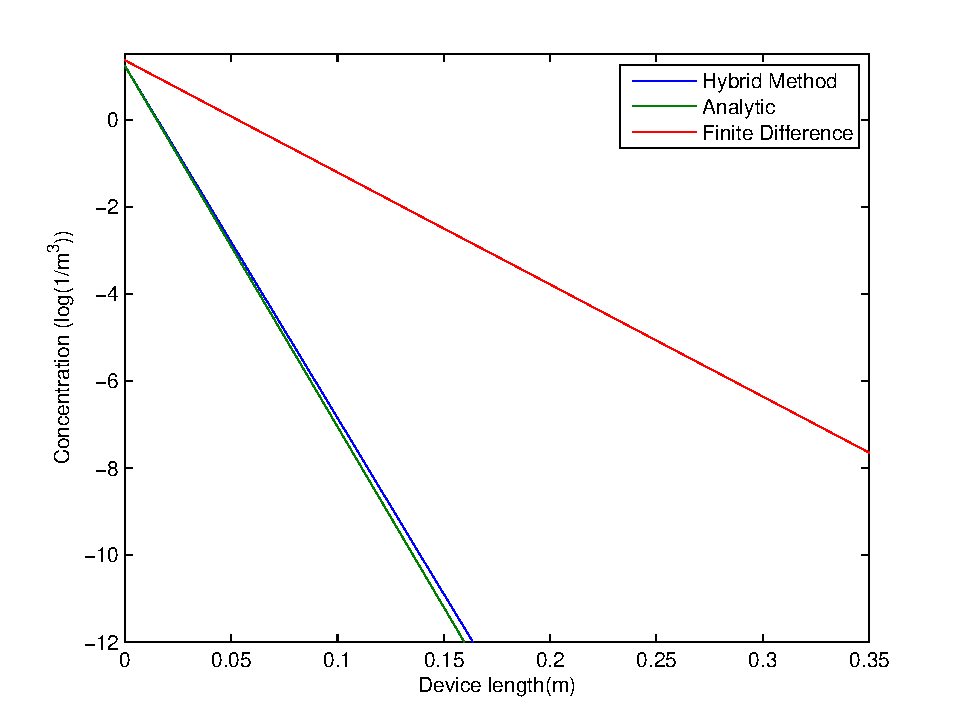
\includegraphics[scale=0.75]{5239}
\caption{Steady State Carrier Distribution for a Drift Dominant Problem} 
\label{61}
\end{figure}

\clearpage
\section{PN Junction}
In previous sections of this chapter we have put finite difference drift diffusion model to test. In all the cases we ran before, Poisson's equation was not coupled with drift diffusion equations. In this example we will be testing both drift diffusion and Poisson's equation to see how well they work when they are coupled together. A simple pn junction is quite adequate for this task since it has analytical solutions, under certain assumptions, for electric potential, electric field and net charge.

For the simulation ,the initial hole and electron distributions were determined using mass action law and they were assumed to be constant at the boundaries. Keeping carrier concentrations constant at the boundaries creates a mechanism in which the charge can move in and out of the simulation domain. If the charge density at any time step is higher than the fixed density then the difference will move out of the system. If there is a lack of charge at the boundary then carriers will move in to fill in the gap. Following figure (\ref{npcon}) shows the final result of bringing p and n type materials together. 
 
\begin{figure}[ht]
\centering
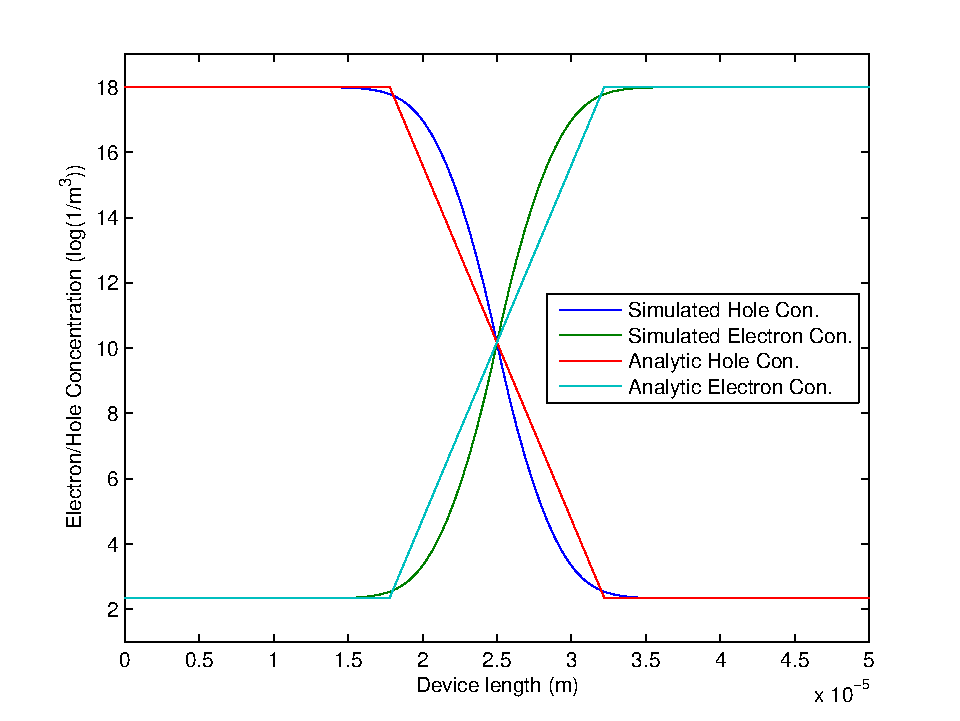
\includegraphics[scale=0.8]{5311}
\caption{Electron/hole Concentration of a PN Junction} 
\label{npcon}
\end{figure}

We can see a little mismatch between simulated and analytic concentration densities. Analytic solution have sharp edges and simulated solution does not. This is due to all the assumptions made in order to find an analytic solution. We will be seeing this little mismatch also for electric field, electric potential and net charge .

Since the purpose of this problem is to test Poisson's equation as well, we can look at the final potential distribution due to pn junction. Figure \ref{pnpot} shows the potential distribution for simulated and analytic solution. Close match in electric potential distribution shows that coupled equations can generate fairly accurate solutions.
 
\begin{figure}[!htp]
\centering
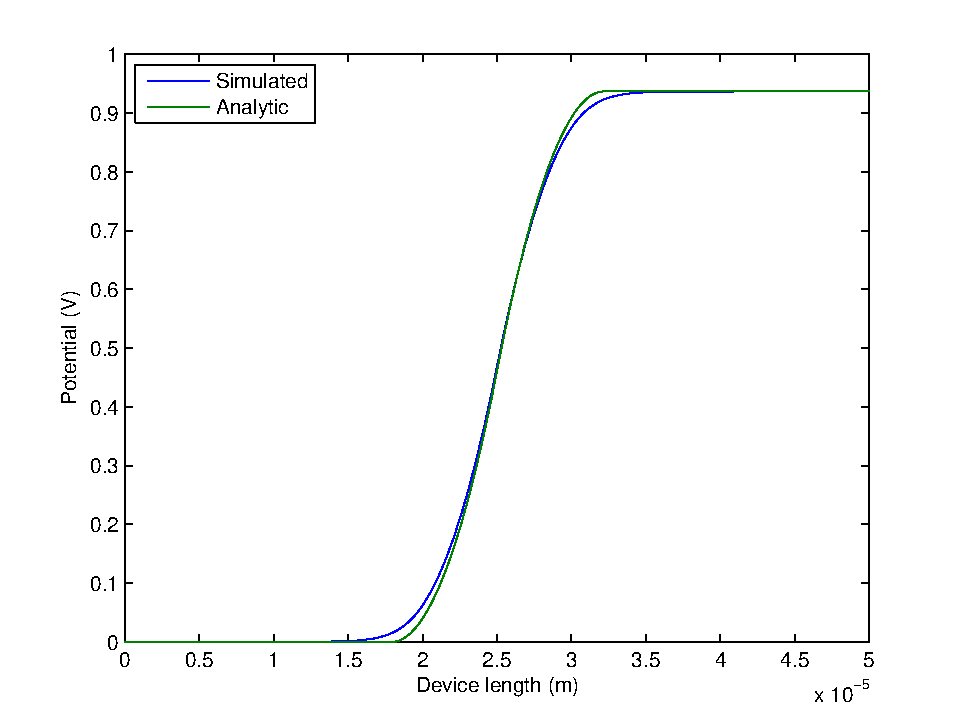
\includegraphics[scale=0.7]{5312}
\caption{Potential Distribution of a PN Junction} 
\label{pnpot}
\end{figure}

Calculation of the electric field involves one basic derivative. Since simulated potential is matching the analytic solution quite nicely the electric field should follow a similar pattern. Figure \ref{pnefield} shows that this is indeed the case, simulated electric field matches the calculated electric field.
\begin{figure}[!htp]
\centering
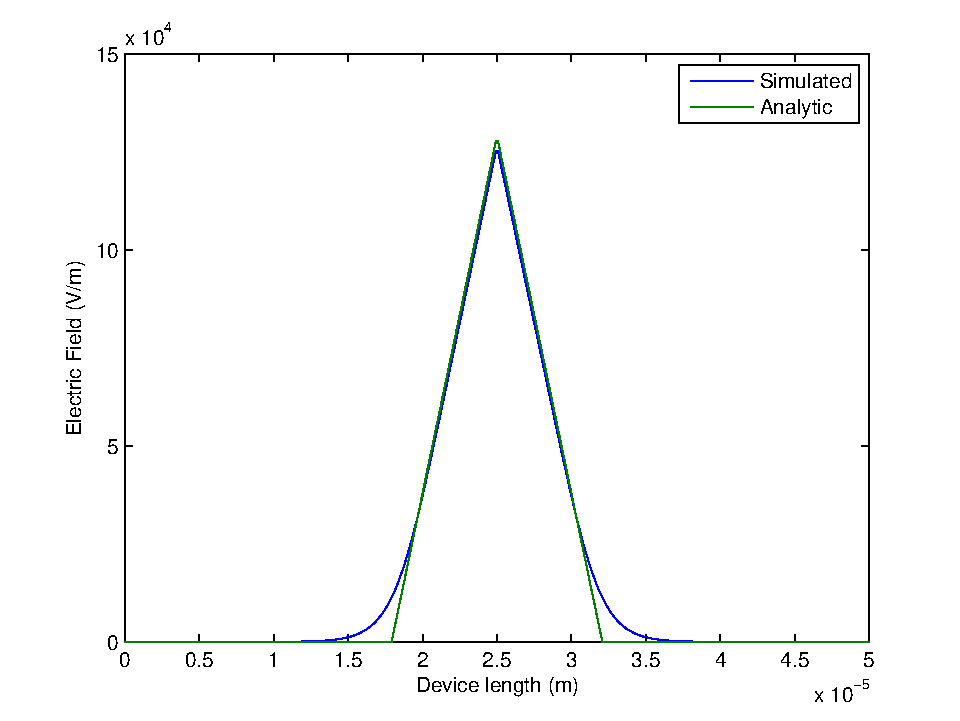
\includegraphics[scale=0.7]{5313}
\caption{Electric Field Distribution of a PN Junction} 
\label{pnefield}
\end{figure}

Finally we can look at the total charge distribution at steady state(\ref{pncd}). Simulated net charge density follows the analytic one except the abrupt changes at two ends. 
\begin{figure}
\centering
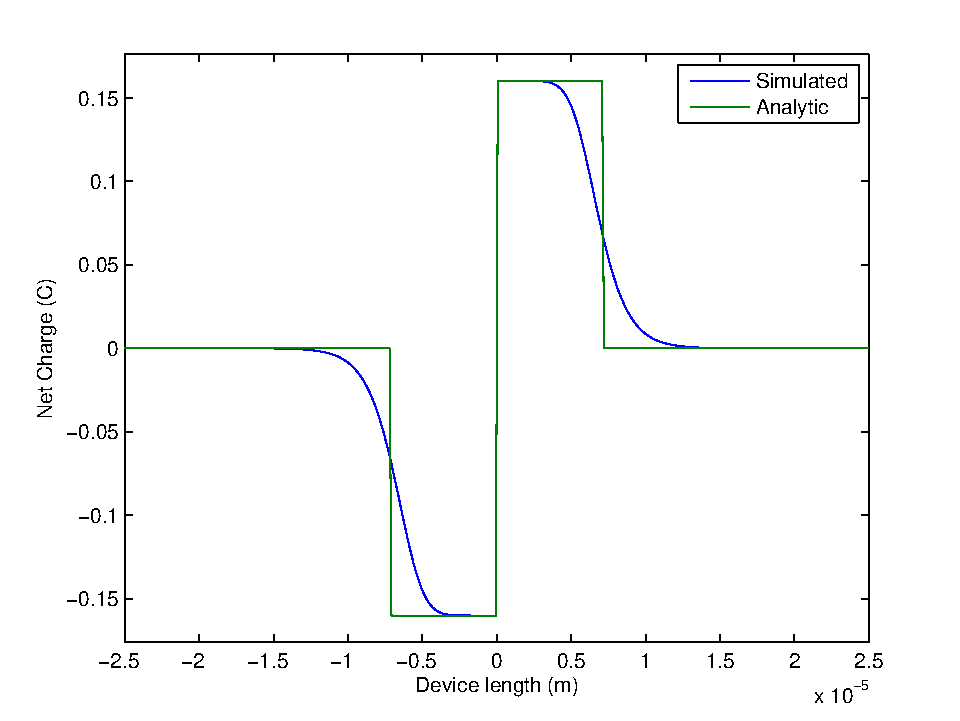
\includegraphics[scale=0.8]{5314}
\caption{Total Charge Distribution of a PN Junction} 
\label{pncd}
\end{figure}




\clearpage
\section{Region Specific Particle Density Limit}

In section 4.2.2.3 we have talked about using a Dirichlet boundary condition (J=0) to stop the particle flow into a node. This can be done by precalculating the particle density of concentration restricted nodes at the next time step, setting any influx to zero if the concentration is going to go over the limit and finally calculating the concentration at the next time step using the updated current densities. 

In order to test this method we can use a simple example where we have two particles of the same charge initialized like the figure below (\ref{5412}). One set of particles has a concentration limit of $2 \; 10^{10} \; m^{-3}$ on the right side of the simulation area and no limit on the left side. The other set has no restrictions.
\begin{figure}[!htp]
\centering
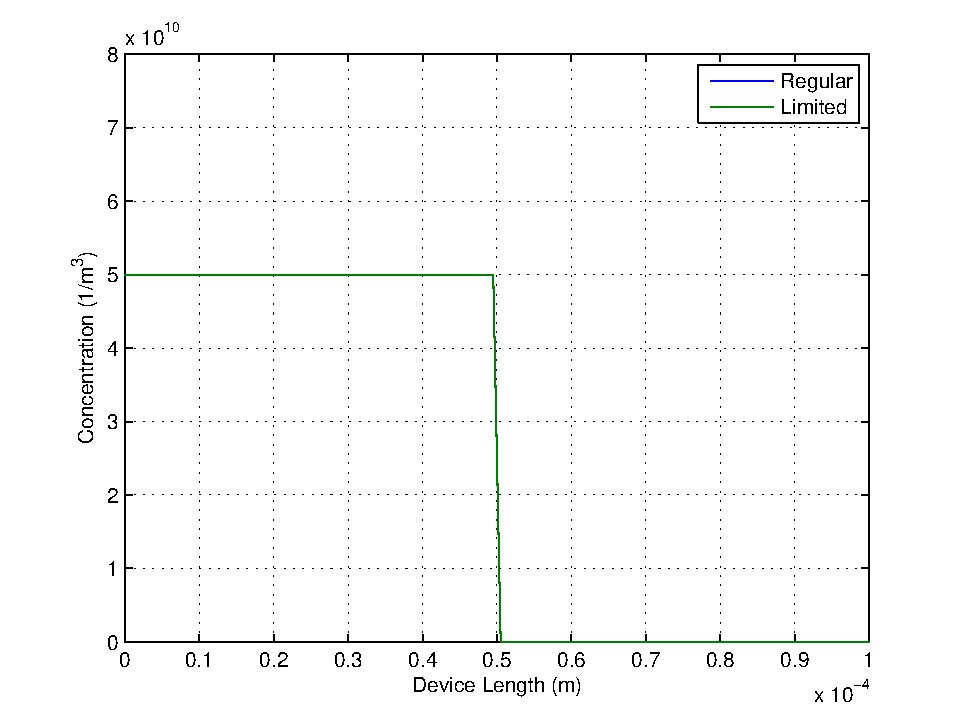
\includegraphics[scale=0.7]{5412}
\caption{Initial Particle Density} 
\label{5412}
\end{figure}

This transient simulation was done using a potential as a function of time. For the first half of the simulation applied potential was positive and for the second half it was negative. Figure \ref{5412} shows how two simulations differ when the particles are pushed towards the right wall due to the electric field created by the positive potential. Particles with no limit on the right side move freely and accumulate on the right side. The limit for the other particles is effectively stopping them from going in and accumulating freely. Once the limit is reached at a certain node the concentration cannot increase any further and that node becomes a no flow wall. 

\begin{figure}[!htp]
\centering
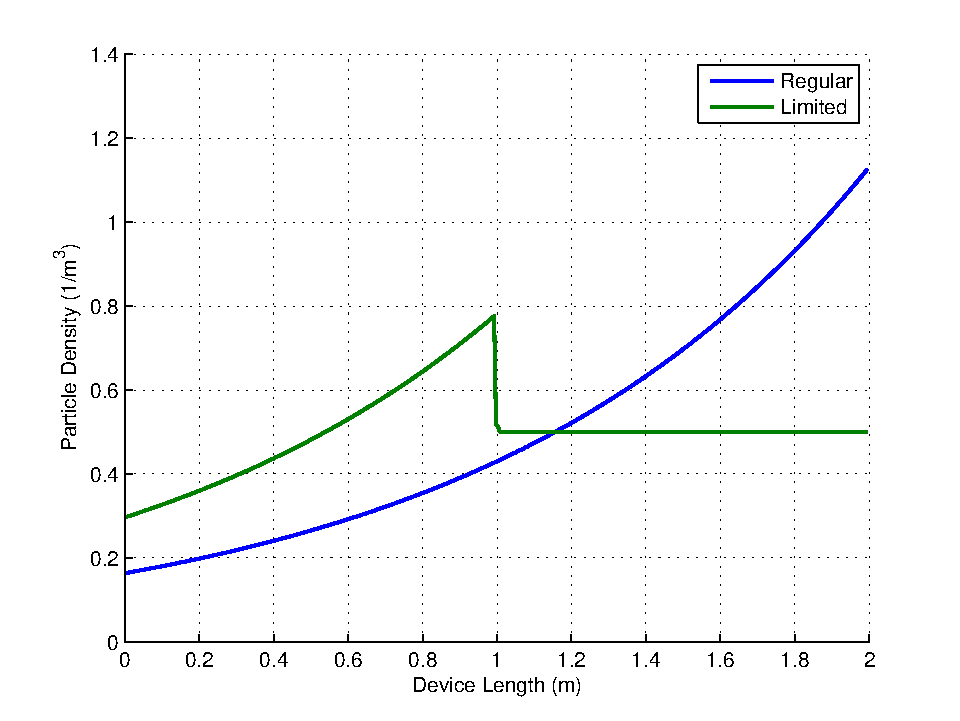
\includegraphics[scale=0.7]{5413}
\caption{Limited Concentration Accumulation on the Right Side} 
\label{5413}
\end{figure}

When the potential is switched all the particles accumulate freely to the left side of the simulation domain since there are no restrictions on this side (figure \ref{5414}).
\begin{figure}[!htp]
\centering
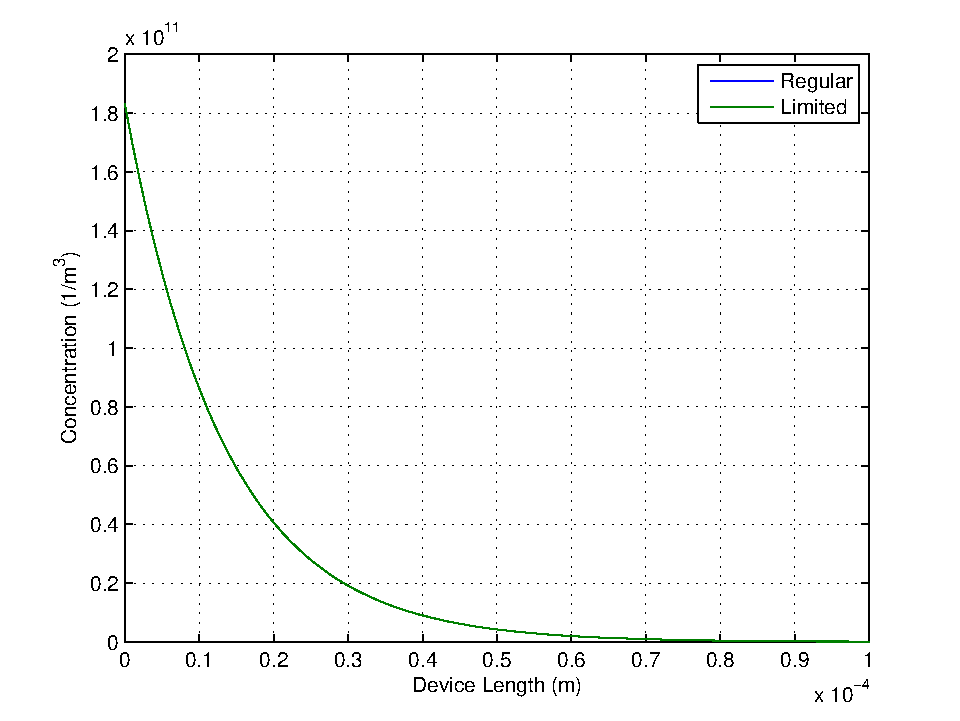
\includegraphics[scale=0.7]{5414}
\caption{Limited Concentration Accumulation on the Left Side} 
\label{5414}
\end{figure}

This last figure (\ref{5411}) shows the transient response  over time of a single node on the right side. The potential is positive for the first 1.5 seconds and it is switched to negative for the last 1.5 seconds. The node without limit keeps accepting charge until steady state has been reached but the node with a limit on stops accepting charged particles once the limit is reached. After the potential is switched density limited node has no problem releasing the particles.


\begin{figure}[!htp]
\centering
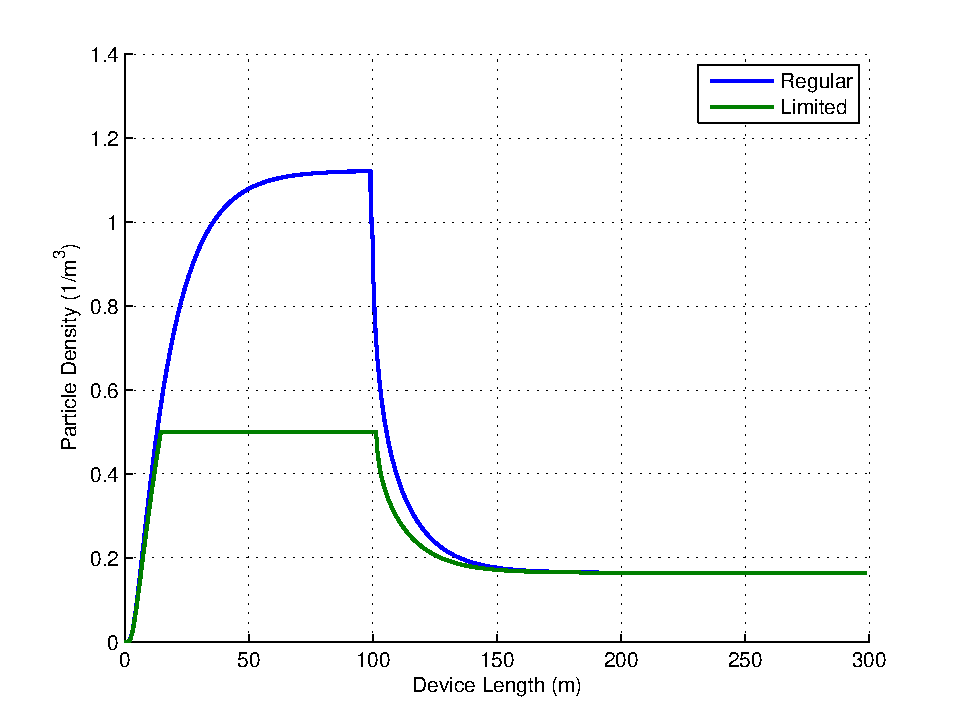
\includegraphics[scale=0.7]{5411}
\caption{Accumulation at the right wall over time} 
\label{5411}
\end{figure}

Additional to the test we ran using finite difference we can also try to simulate the exact same behaviour in COMSOL. 

COMSOL does not have a built in option that allows limiting particle density. One possible solution to this is making particle mobility and diffusivity a function particle density. It is possible to use a sigmoid function which switches from 1 to 0 very quickly when particle density is close to its limit. Here is the equation of the sigmoid function used to limit the particle flow:

\begin{equation}
\mu = \frac{\mu_{0}}{1+e^{\sigma(n-n')}}
\label{mur}
\end{equation} 

$\mu_0$ is the original mobility of the charge carrier. $\sigma$ controls the sharpness of the switch and $n'$ determines the density at which the switch will be. 

Another problem with COMSOL was the definition of mobility and diffusion coefficients over different areas. If these constants are defined as one single value per area it works just fine but if they are defined as a function of concentration it causes convergence issues. This can be overcome by defining using two more sigmoid functions to distinguish between two areas with different mobilities and diffusion constants. Left sigmoid in figure \ref{5420}  was multiplied by the mobility/diffusivity of the left side of the area and the right sigmoid was multiplied by the mobility/diffusivity of the right side of the area. Both functions were summed to obtain a function which describes the characteristics of the entire area.

\begin{equation}
\mu=\frac{\mu_{l}}{1+e^{\sigma_x(x-x')}}+\frac{\mu_{r}}{1+e^{-\sigma_x(x-x')}}
\end{equation}

In this problem $\mu_r$ is the same as equation \ref{mur} since the region on the right side has a particle density limit. A sharp switch between right and left side mobility using the function above would be ideal for this simulation but unfortunately it causes convergence issues in COMSOL therefore there is a gradual change between two mobilities. 

\begin{figure}[!htp]
\centering
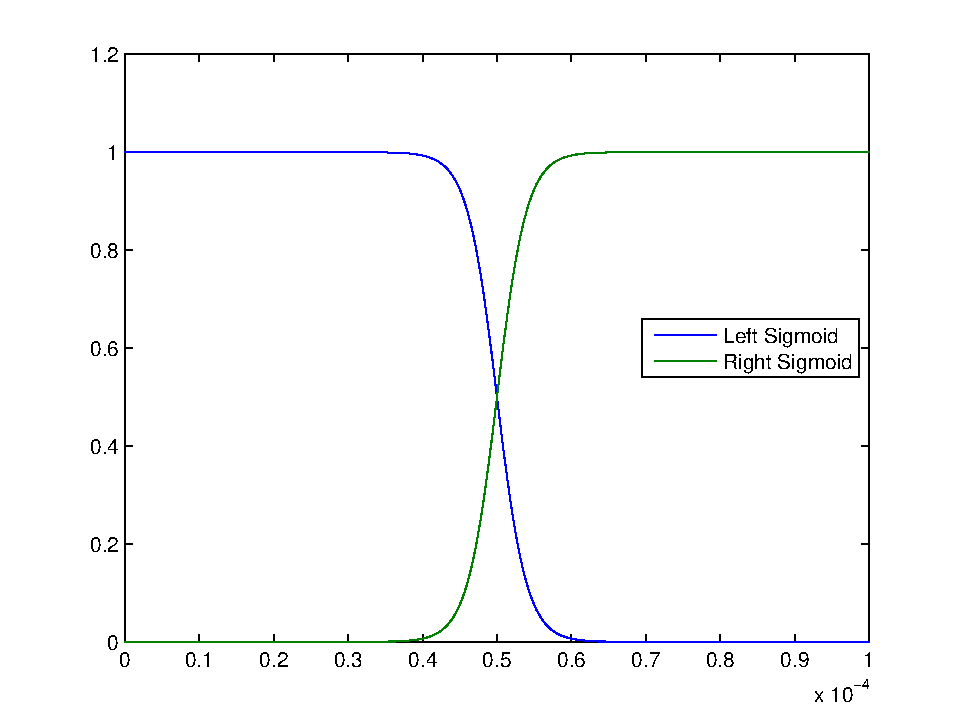
\includegraphics[scale=0.7]{5420}
\caption{Mobility change from left to right side} 
\label{5420}
\end{figure}

The initial carrier distribution for COMSOL was set to be exactly the same as finite difference simulation. Figures \ref{5416} and \ref{5423} show results for both COMSOL and finite difference simulations at steady state before the potential switch. The plot on the left side gives insight on how COMSOL simulation behaves for limited and limitless accumulation on the right wall. Due to the gradual change of mobility and diffusion constants between two areas we end up with concentration on the right side higher than the limit which is $2 \; 10^{10}$. Additionally, the particle density goes over its limit near the right wall. In figure \ref{5423} the difference between COMSOL and finite difference becomes more visible. In FD simulation the accumulation goes much higher due to higher electric field and unlike COMSOL it does not penetrate the right half of the simulation domain. 

\begin{figure}[ht]
\centering
\begin{minipage}[b]{0.45\linewidth}
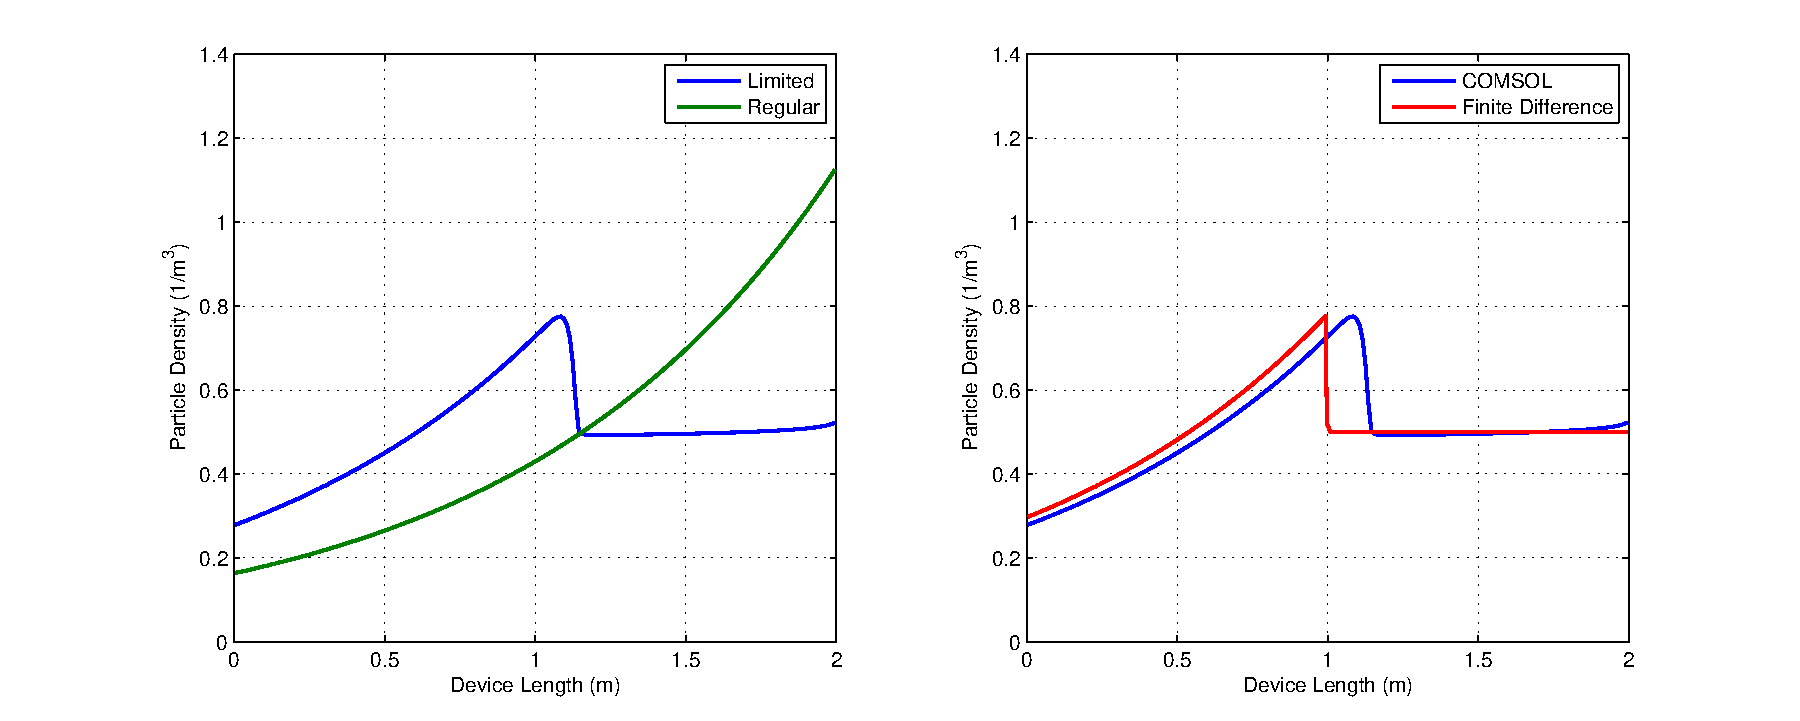
\includegraphics[scale=0.45]{5416}
\caption{COMSOL Simulation for Particle Density Limit}
\label{5416}
\end{minipage}
\quad
\begin{minipage}[b]{0.45\linewidth}
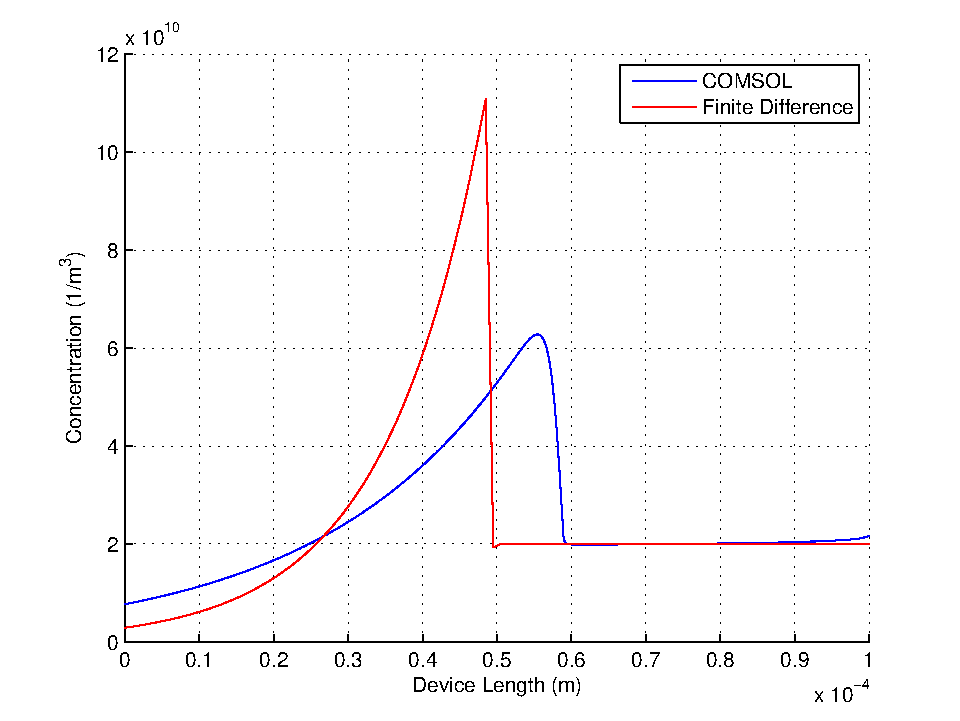
\includegraphics[scale=0.45]{5423}
\caption{COMSOL and Finite Difference Simulation}
\label{5423}
\end{minipage}
\end{figure}


In figure \ref{5417} we can see the accumulation of charge near the middle after the potential is switched. This is due to mobility being a function of distance and concentration. As the ions move from left to right they go from a low mobility region to a high mobility region and they slowly accumulate around the area where the change in mobility occurs. Figure comparing both COMSOL and finite difference shows that the accumulation does not happen in the case of finite difference due to the way concentration limiting mechanism was implemented.

\begin{figure}[ht]
\centering
\begin{minipage}[b]{0.45\linewidth}
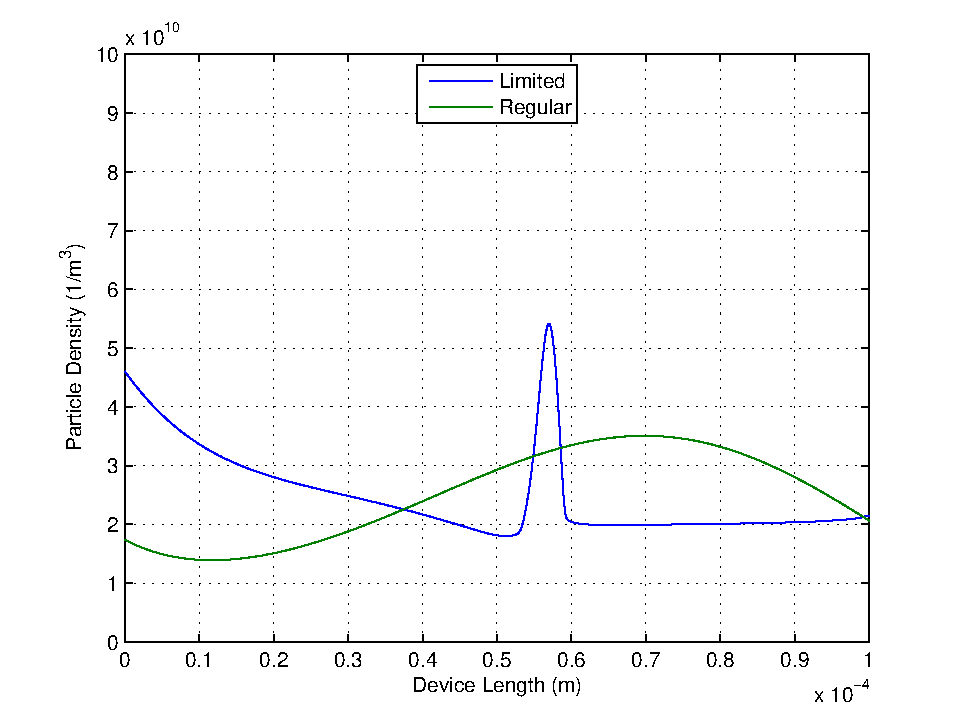
\includegraphics[scale=0.45]{5417}
\caption{COMSOL Simulation for Particle Density Limit}
\label{5417}
\end{minipage}
\quad
\begin{minipage}[b]{0.45\linewidth}
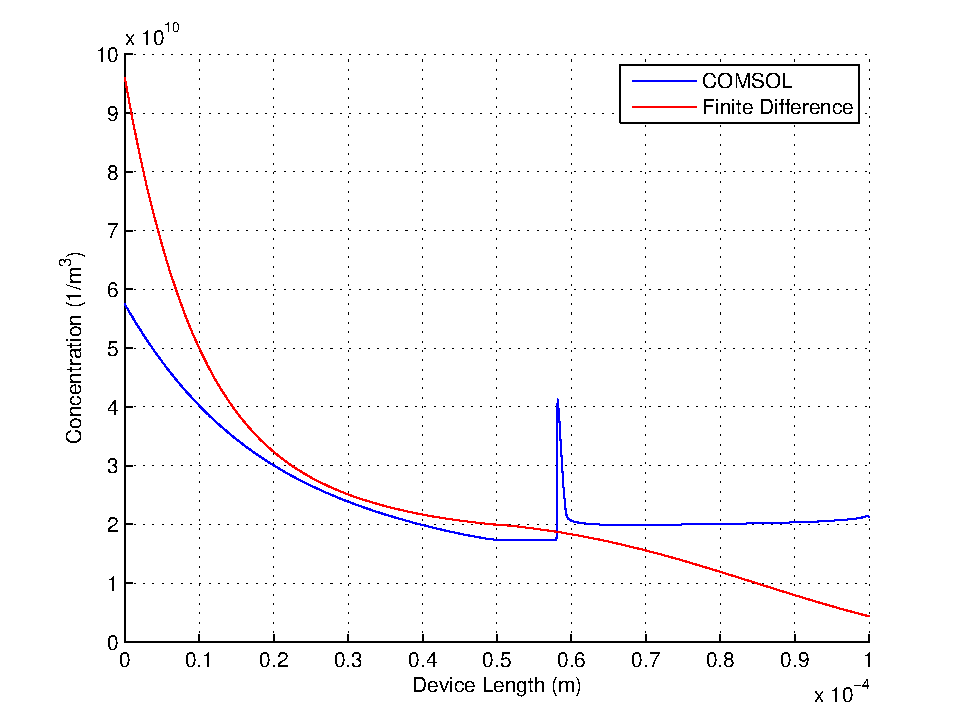
\includegraphics[scale=0.45]{5424}
\caption{COMSOL and Finite Difference Simulation}
\label{5424}
\end{minipage}
\end{figure}

With the decrease of ion concentration on the limited region the difference between low and high mobility regions diminish. Once the concentration on the limited side is low enough the whole system behaves as if there was no limit and ion mobility becomes equal for all regions and the ions freely accumulate on the left wall (figure \ref{5418}). Aside from the difference in electric field strength both simulations behave the same way as they approach steady state. Figure \ref{5426} shows concentration densities at steady state. COMSOL simulation has a lower electric field since it has convergence issues with high electric fields. 

\begin{figure}[ht]
\centering
\begin{minipage}[b]{0.45\linewidth}
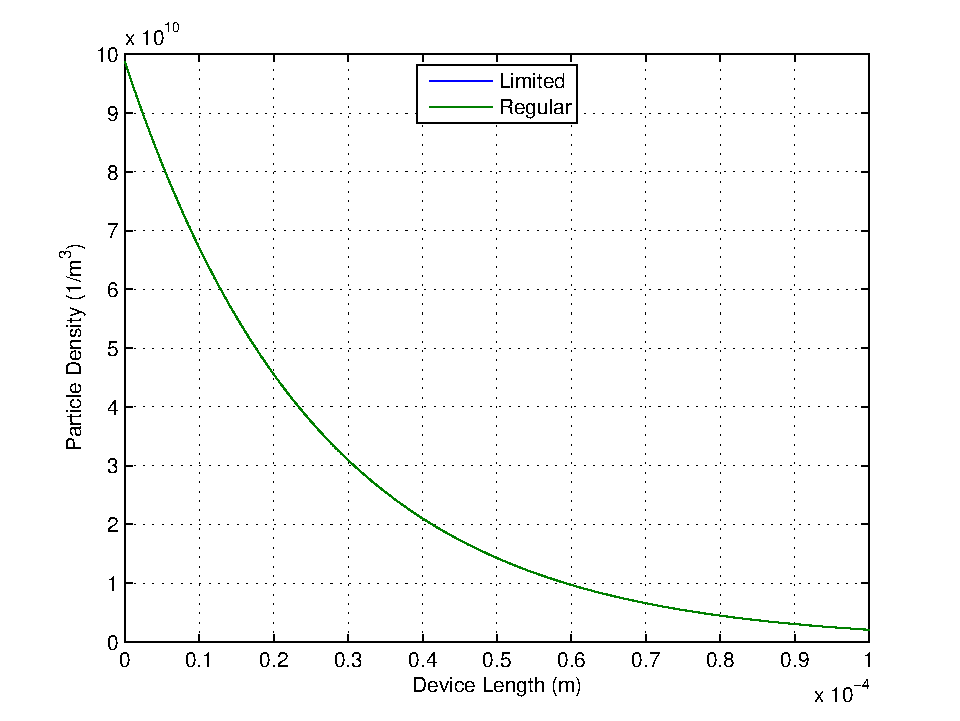
\includegraphics[scale=0.45]{5418}
\caption{COMSOL Simulation for Particle Density Limit}
\label{5418}
\end{minipage}
\quad
\begin{minipage}[b]{0.45\linewidth}
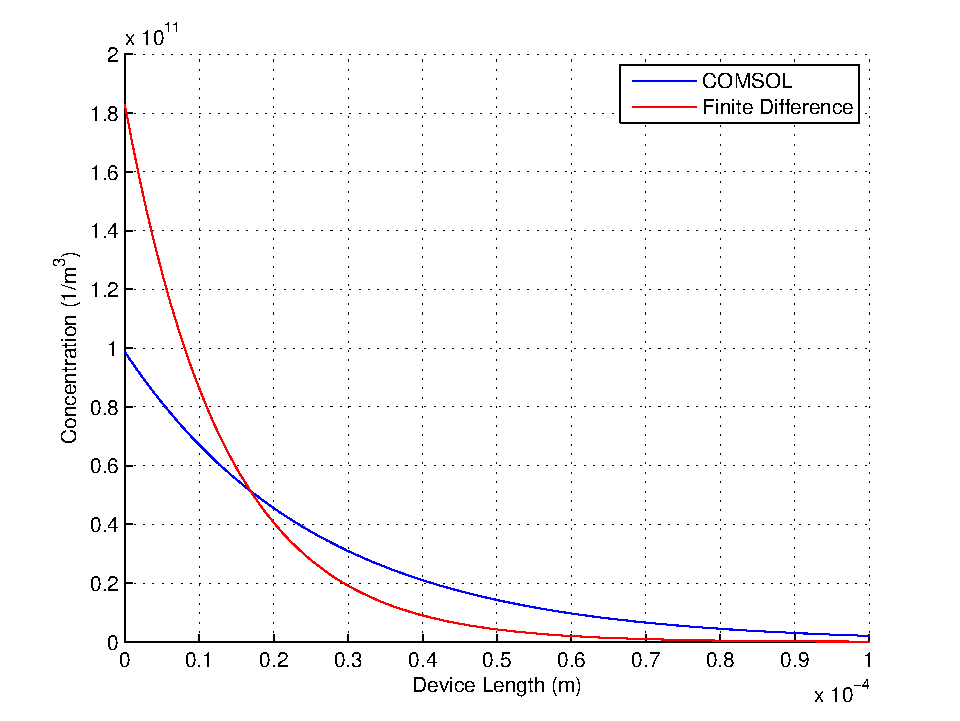
\includegraphics[scale=0.45]{5426}
\caption{COMSOL and Finite Difference Simulation}
\label{5426}
\end{minipage}
\end{figure}

To finish our comparison we can look at the particle density transient response of the rightmost node. For the first half of the simulation everything is the same as the finite difference case except COMSOL goes a little bit over the limit. When the potential is switched node without the limit has no noticeable difference in behaviour. The node with concentration limit has a lag when it comes to releasing the particles. This is due to the sigmoid function used to achieve a limiting behaviour. Once the limit is reached mobility and diffusivity are stuck at a very low value until the particle density starts to go lower than the limit.
\begin{figure}[ht]
\centering
\begin{minipage}[b]{0.45\linewidth}
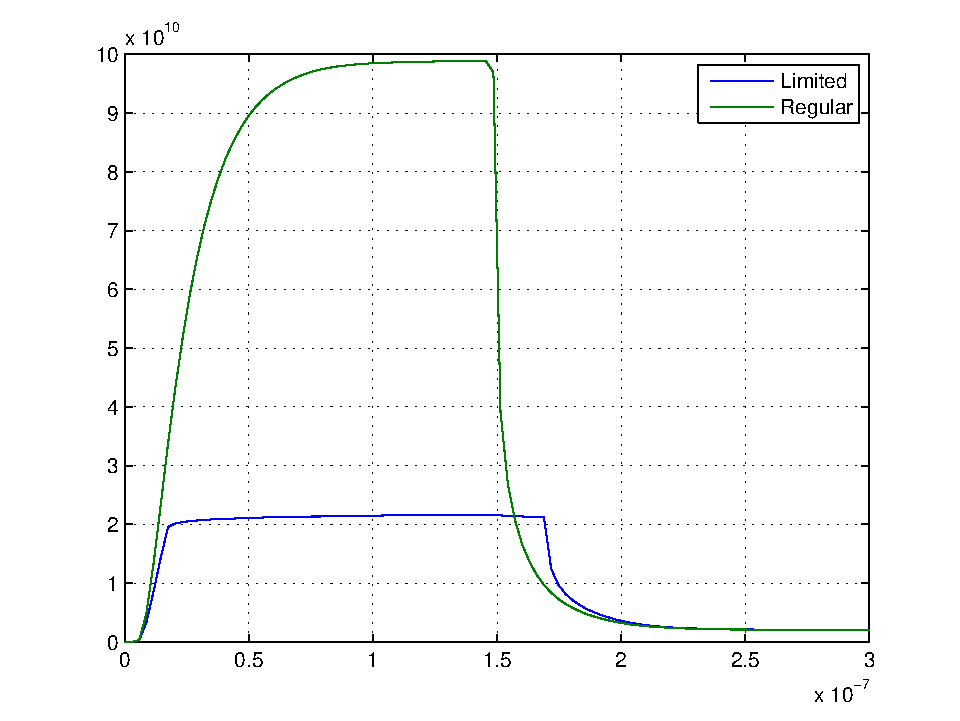
\includegraphics[scale=0.45]{5419}
\caption{Density on the right wall over time using COMSOL}
\label{5419}
\end{minipage}
\quad
\begin{minipage}[b]{0.45\linewidth}
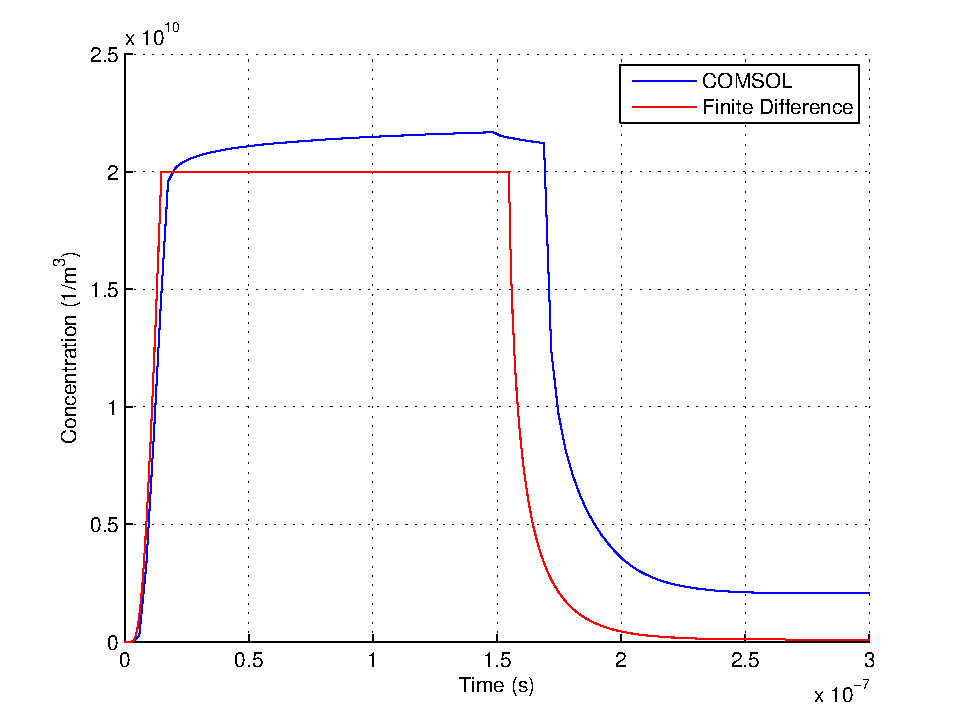
\includegraphics[scale=0.45]{5421}
\caption{Density on the right wall over time,COMSOL vs. Finite Difference}
\label{5421}
\end{minipage}
\end{figure}

In this example we have seen that it is possible to impose a density limit over any area using a simple no flow boundary condition in finite difference. For COMSOL we had to use some workarounds in order to simulate the same behavior but the results were not very satisfying because of convergence issues. 
% Chapter Template

\chapter{Memristor Simulation} % Main chapter title

\label{Chapter5} % Change X to a consecutive number; for referencing this chapter elsewhere, use \ref{ChapterX}

\lhead{Chapter 5. \emph{Memristor Simulation}} % Change X to a consecutive number; this is for the header on each page - perhaps a shortened title

A numerical method for a memristor simulation was developed and tested in previous chapters based on drift-diffusion equations and finite difference. This chapter introduces the memristor's structure and physical parameters used for the simulation. It continues with a preliminary problem analysis to determine required mesh density and maximum possible time step. This preliminary analysis is followed by 1-D simulations of 3 different cross sections of a memristor.

\section{Memristor Structure}
%-Problem Analysis and assumptions, semiconductor vs memristor plots
Following figure (\ref{MemStc}) shows the structure of a simple memristor which will be taken as a basis for all the memristor simulations presented in this thesis. It consists of 2 metal contacts a polymer conductor (PEDOT:PSS) and an electrolyte solution which has lithium and perchlorate ions (6.02 $10^{26} m^{-3}$). The memristor is about 1 cm long. The thickness of the conductive layer is around 1 $\mu$m. During experimentation the electrolyte is deposited on PEDOT via a syringe so its thickness can vary drastically but as long as the amount of ions in the electrolyte solution is enough to saturate PEDOT this does not make a significant difference in the operation of the memristor. For simulation it was assumed that there were always more than enough ions to saturate the PEDOT so the electrolyte was modeled as an infinite source/sink of ions. The top boundary of the electrolyte was assumed to be charge neutral at all times which provides a mechanism for moving ions in and out of the system. This way the movement of ions near the surface of the PEDOT can still be captured without having to simulate the ion movement for the entire electrolyte solution which is variable in size. 

\begin{figure}[!htp]
\centering
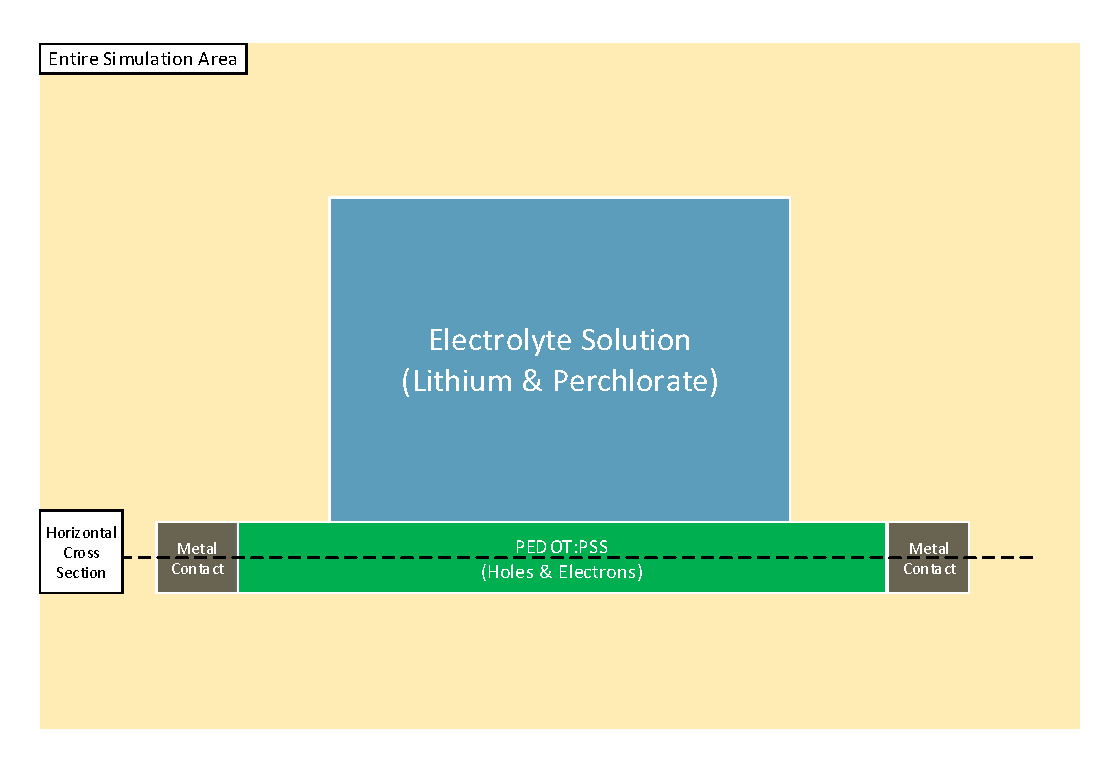
\includegraphics[scale=0.50]{Mem1}
\caption{} 
\label{MemStc}
\end{figure}

The initial conditions for all the charge carriers are the same. All charge are balanced and uniformly distributed but the carrier density in the electrolyte solution is higher than the carrier density in PEDOT. Perchlorate ions are not allowed to move outside the electrolyte solution so a no flow boundary condition was used around the electrolyte. Lithium ions are free to move between PEDOT and the electrolyte solution but their maximum concentration is limited inside the PEDOT. The mobility of lithium ions has further restrictions inside PEDOT. Lithium has higher mobility in region of PEDOT under the electrolyte solution, wet PEDOT, than the region without any contact with electrolyte, dry PEDOT. In fact due to this difference very little amount of lithium reaches the metal contacts. This decrease in mobility was modeled by making the mobility of lithium a function of position. The mobility of lithium ions were assumed to be 100 times slower than the mobility of holes ( $\approx$ $10^{-4}$ $m^2/Vs$).  

PEDOT:PSS is a regular conductor with fixed negative charge and mobile holes. Holes can move in an out of the PEDOT through the metal contacts which hold the charge neutrality of the initial condition throughout the simulation. The interface between PEDOT and electrolyte only allows the exchange of lithium ions. During simulation,the movement of lithium ions changes the conductivity of the PEDOT by increasing or decreasing the amount of available holes through coulomb forces. In the actual device lithium ions change the conductivity via various physical effects like changing the mobility of holes through modifying their hopping distance. These additional affects are beyond the scope of this thesis. 


\clearpage
\section{Simulation Requirements}

It is important to analyze computational requirements of a simulation in order to asses the feasibility of the computation scheme. It is possible to determine these spacial and temporal requirements using the equations \ref{debye} to \ref{CFL_Drift} which describe physical and numerical limitations of the simulation. Following graph \ref{SpaceTime} shows the requirements for a memristor of the scale discussed above and a typical semiconductor device around 1 $\mu$m. The mesh density has to be high enough in order to capture the exponential charge accumulation for charge shielding so the minimum step size was set to be 5 times the Debye length. Plots \ref{SpaceTime}.a and \ref{SpaceTime}.c show the amount of points required to simulate a semiconductor and a memristor based on minimum step size. It is important to note that these values are for 1-D simulation and they can be converted to 2-D and 3-D by squaring or cubing y axis values respectively. Plots \ref{SpaceTime}.b and \ref{SpaceTime}.d were created using CFL conditions for drift and diffusion and dielectric relaxation time. A typical simulation time was estimated using mobility and electric field. Based on the estimated simulation time the number of time steps were calculated using the minimum time step obtained from CFL conditions and dielectric relaxation time.

It can be seen from graphs \ref{SpaceTime}.a and \ref{SpaceTime}.c that memristor simulations require much higher mesh densities compared to a typical semiconductor simulation. This is due to the larger size and higher charge density of the memristor. Graph \ref{SpaceTime}.a \ref{SpaceTime}.b show that a memristor with $10^{26}$ $m^{-3}$ charge density of the electrolyte would require close to $10^9$ points and $10^{14}$ time steps to simulate in 1-D. These requirements make the simulation of the memristor extremely challenging. One possible solution to this problem is to use a much lower charge density and assume that all the values scale linearly. Following cross sectional simulations (Figure \ref{MemStc}) were made to determine the effect of increasing charge density on memristor simulations and to investigate if scaling can be used without compromising the reliability of the simulation.

\begin{landscape}
\begin{figure}[htp]
\centering
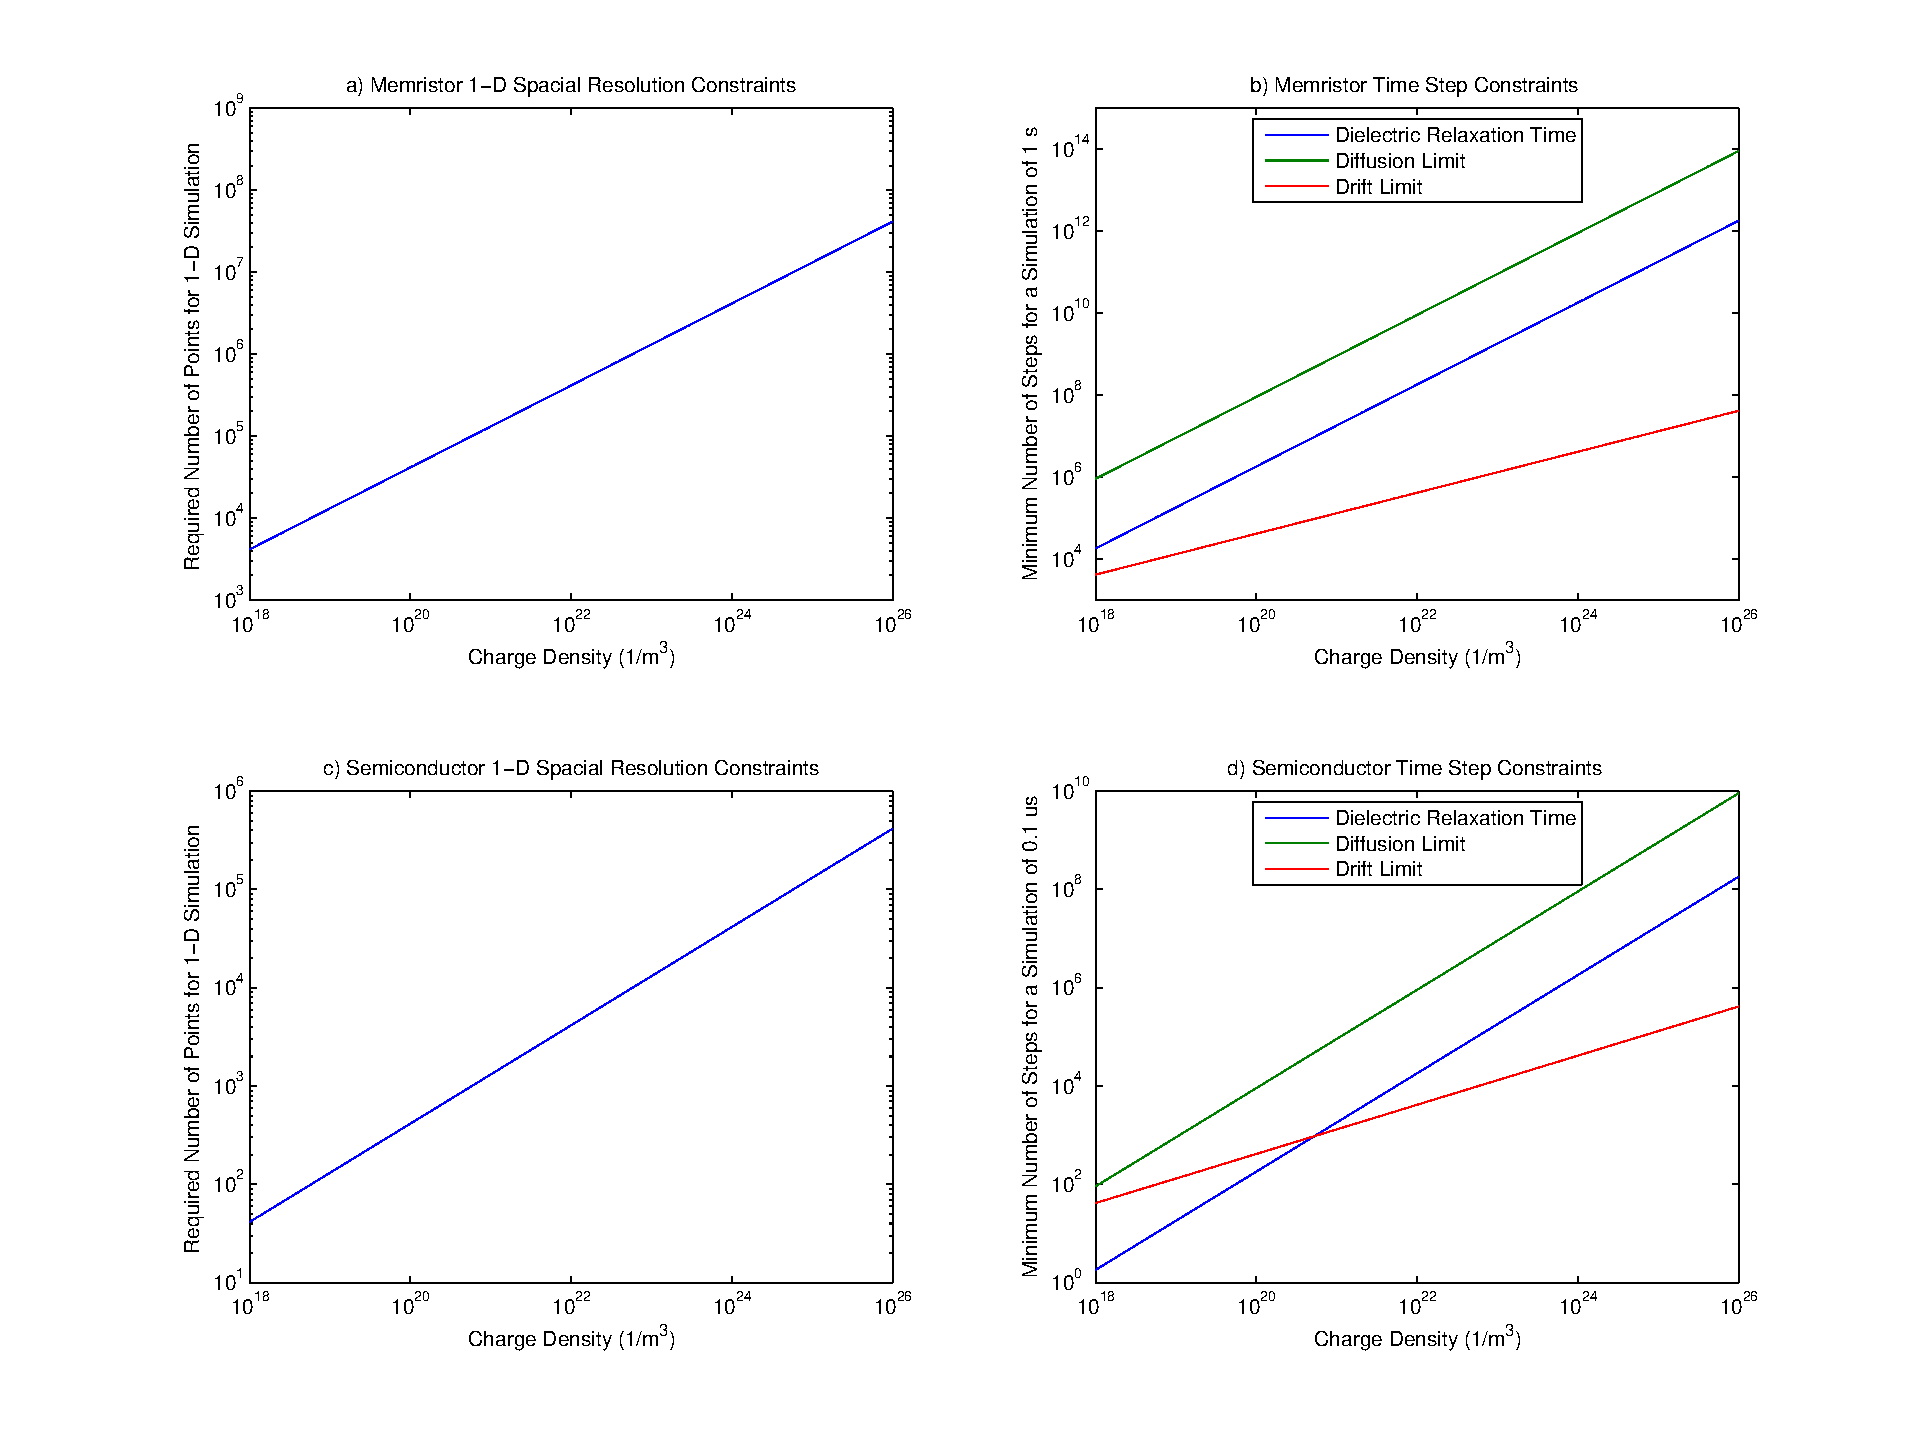
\includegraphics[scale=0.60]{SpaceTime}
\caption{Spatial and temporal requirements for simulation} 
\label{SpaceTime}
\end{figure}
\end{landscape}

\clearpage
\section{Memristor Cross Sectional Simulations}

Even though it is possible to simulate the structure presented in section 5.1 in 2-D, simulating cross sections of the memristor separately has a major advantage. The purpose of these preliminary  simulations is to test the affect of various charge densities which requires mesh density to be as high as possible. Increasing mesh density in 1-D has a smaller impact on computational load therefore higher charge densities are more accessible.  

In following 1-D simulations initial carrier densities ranging from $2$ $10^{15}$ $m^{-3}$ to $10$ $10^{15}$ $m^{-3}$ were used. Unless otherwise stated the plots for charged particle densities were normalized to $2$ $10^{15}$ $m^{-3}$ in order to show the effect of density scaling. 

\subsection{Electrolyte Simulation (Cross Section 1)}

A steady state and transient solution of the cross section 1 indicated in figure \ref{MemStc} is presented in this section. Positive an negative charges were uniformly initialized at different densities for each simulation and two contacts representing the elctric field generated by the metal contacts of the memristor were placed on each side of the electrolyte. Potential on the metal contacts were kept at 1 V and 0 V on the left and right side respectively. The electrolyte solution has a high density of positive and negatively charged particles. As long as there are enough particles, any electric field inside the electrolyte will be canceled out due to separation of charge. This means that, in a memristor, any electric field due to metal contacts reaching the electrolyte will be canceled out. Following figure (\ref{ElectrolyteQ}) shows the distribution of net charge density in steady state for various initial charge densities.  These plots were not normalized since the net charge required to cancel the electric field is the same for all densities. Naturally, the final charge distribution is almost identical in all cases.

\begin{figure}[htp]
\centering
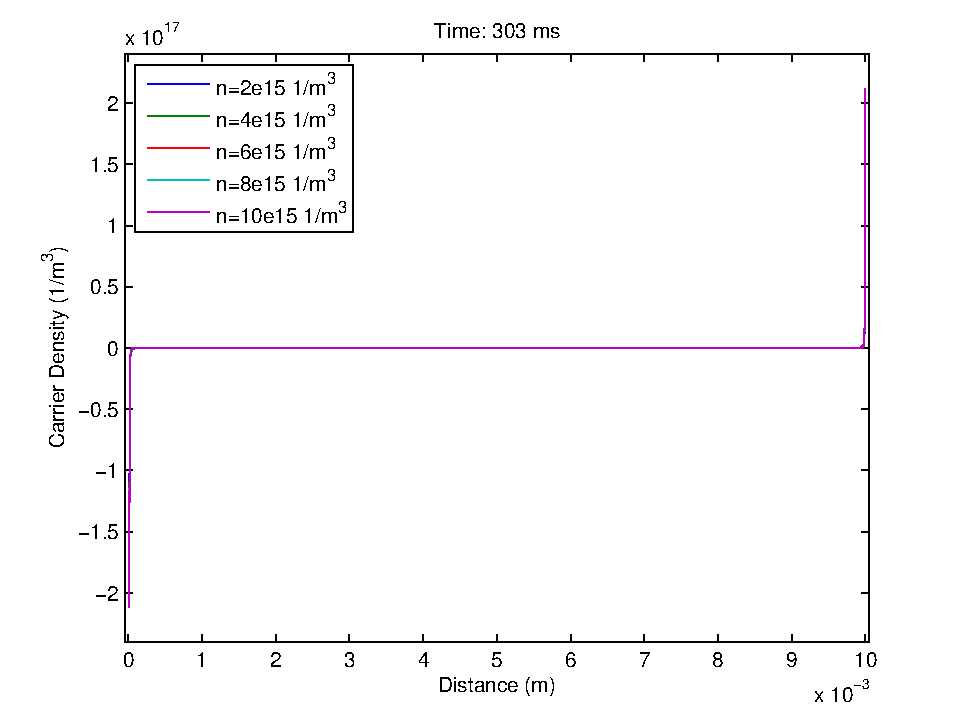
\includegraphics[scale=0.50]{Ex1NetQ_Time_All}
\caption{Final net charge density distribution in electrolyte subject to an electric field} 
\label{ElectrolyteQ}
\end{figure}

Figure \ref{ElectrolyteQzoom} shows the charge accumulation on the right wall over time. It can be seen that the higher the initial charge concentration is the faster it reacts to the applied field. This behavior is expected since with higher charge density less charge needs to move in order to cancel the electric field. This effect can better be seen in figure \ref{ElectrolyteV} which shows the evolution of potential over time. The change in potential over time shows that higher densities cancel out the electric field faster than lower densities.

The inverse relationship between charge density and debye length was given in equation \ref{debye} which can be physically be observed from figure  \ref{ElectrolyteV2}. The distance over which the potential is being canceled out is getting shorter with the increase of charge density.  

 
\begin{landscape}
\begin{figure}[!htp]
\centering
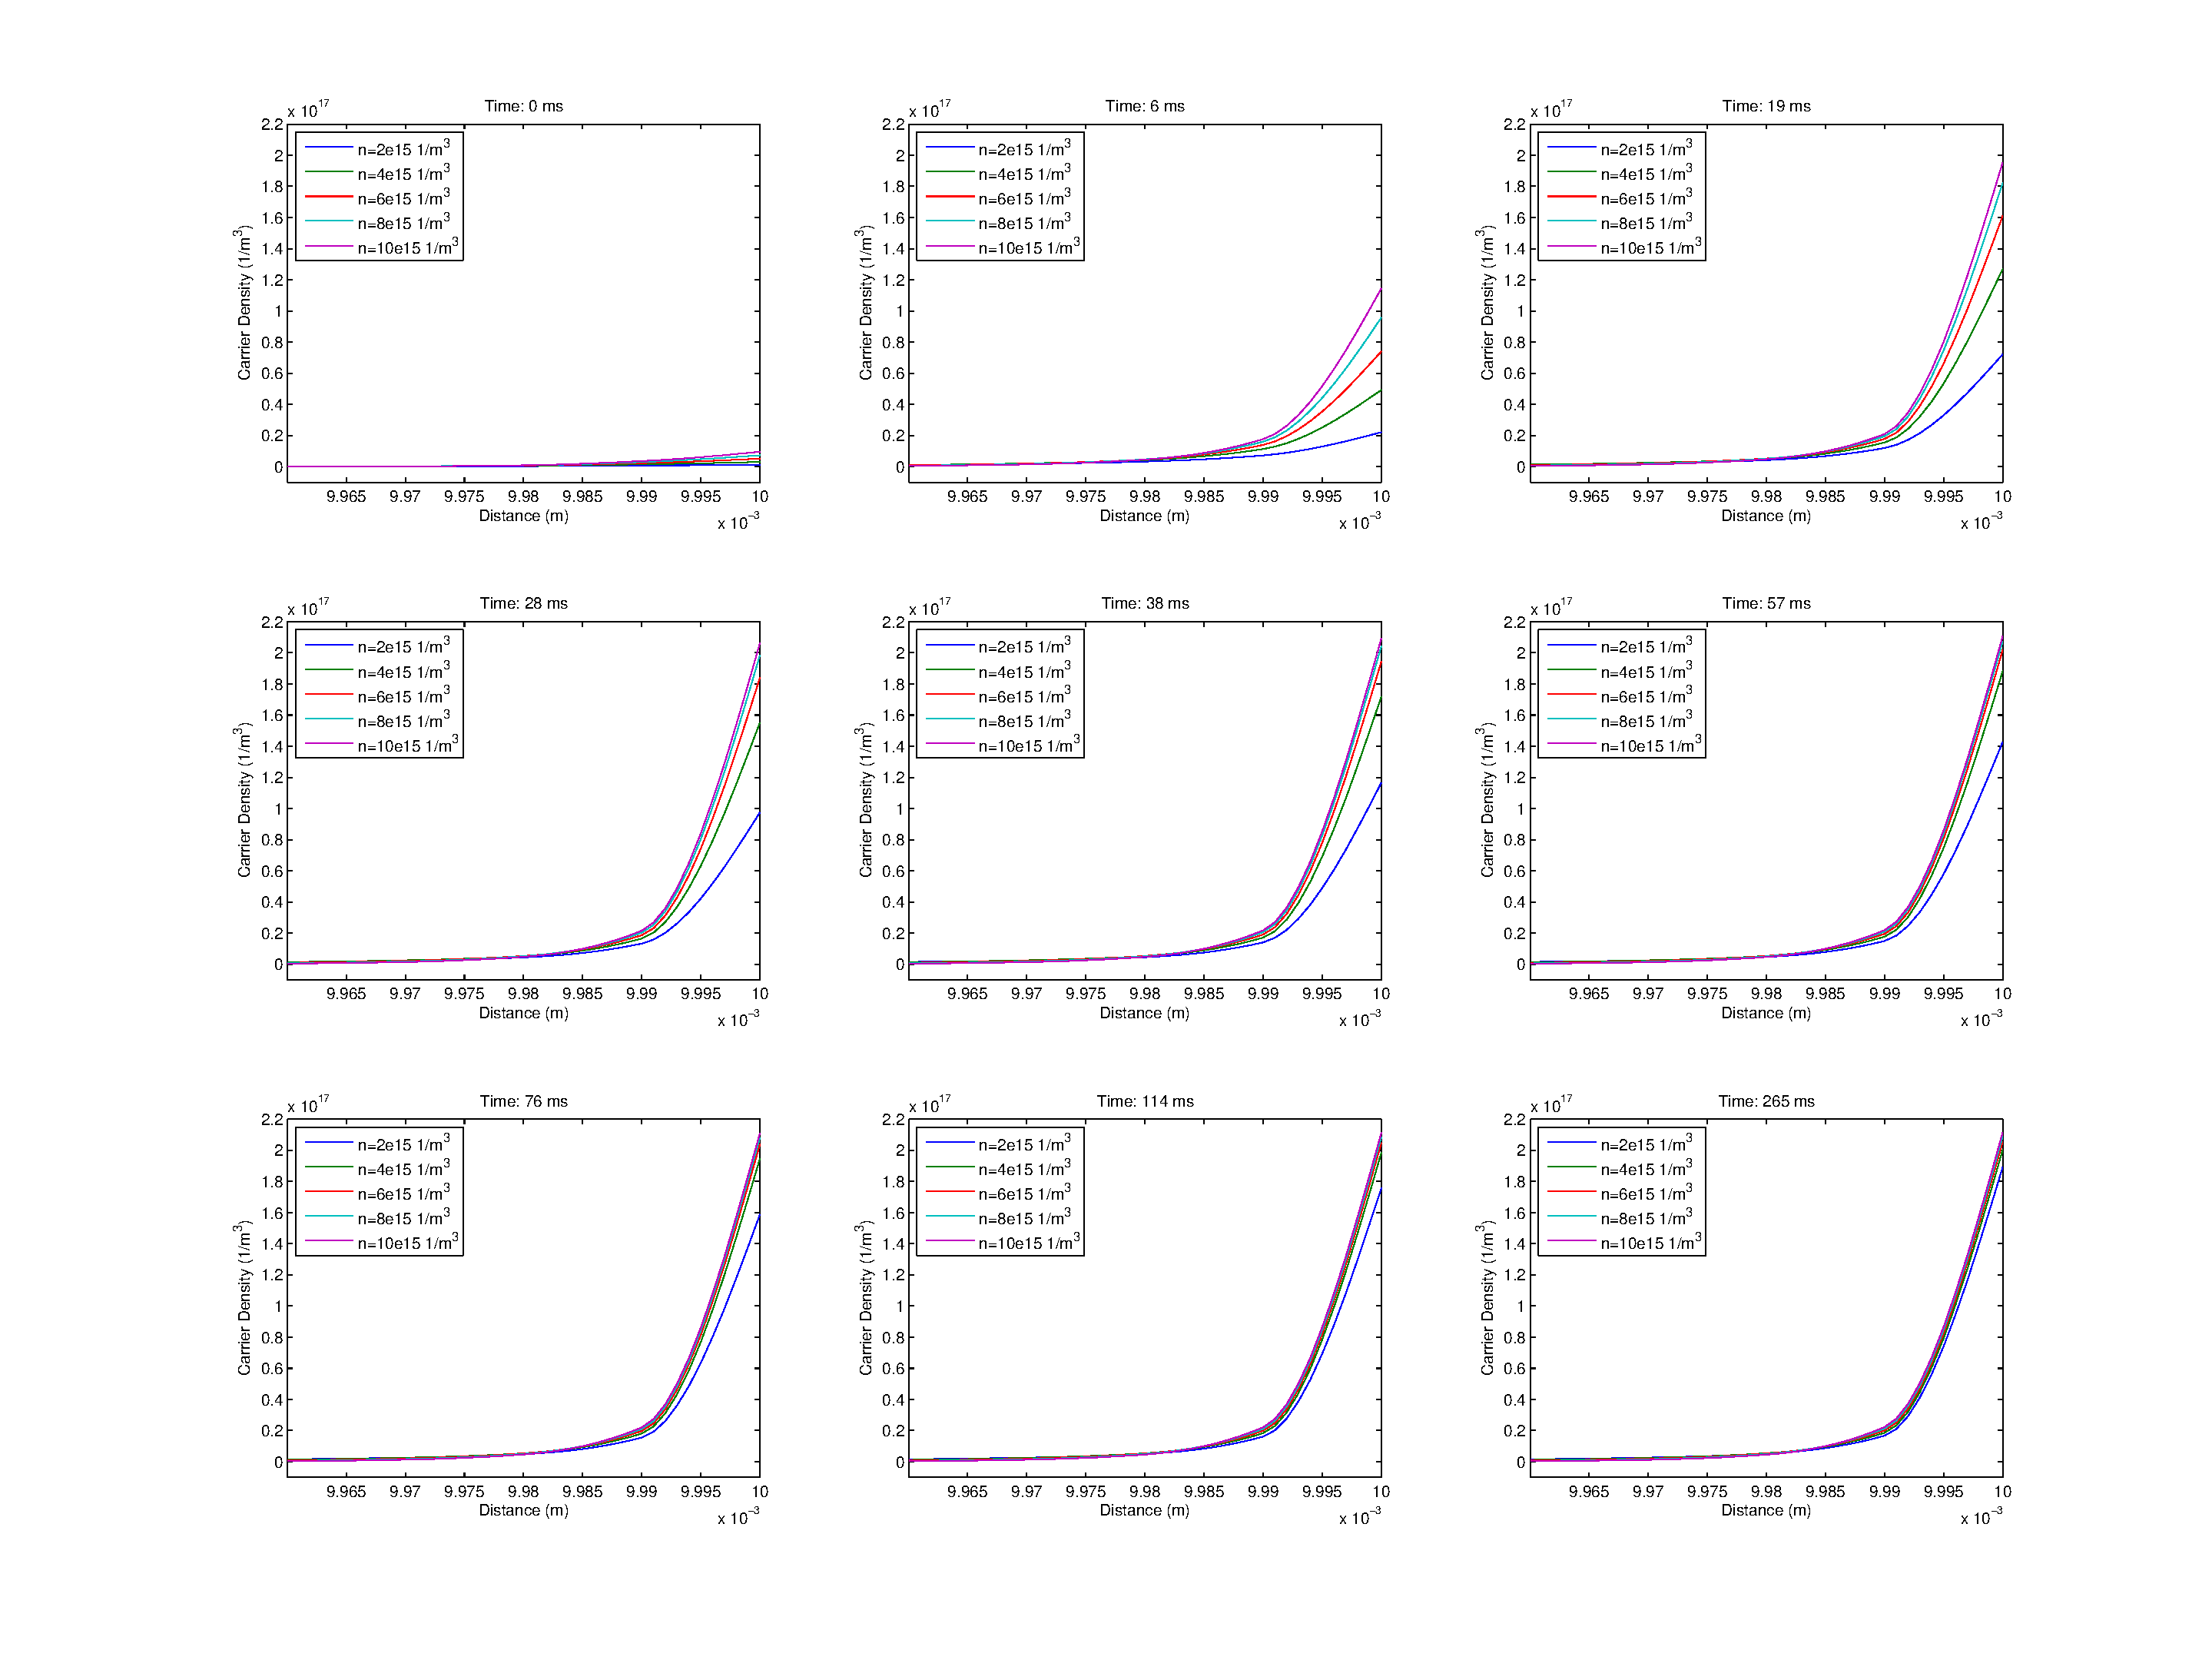
\includegraphics[scale=0.40]{Ex1NetQ_Time}
\caption{Normalized net charge density distribution in electrolyte over time} 
\label{ElectrolyteQzoom}
\end{figure}
\end{landscape}

\begin{landscape}
\begin{figure}[!htp]
\centering
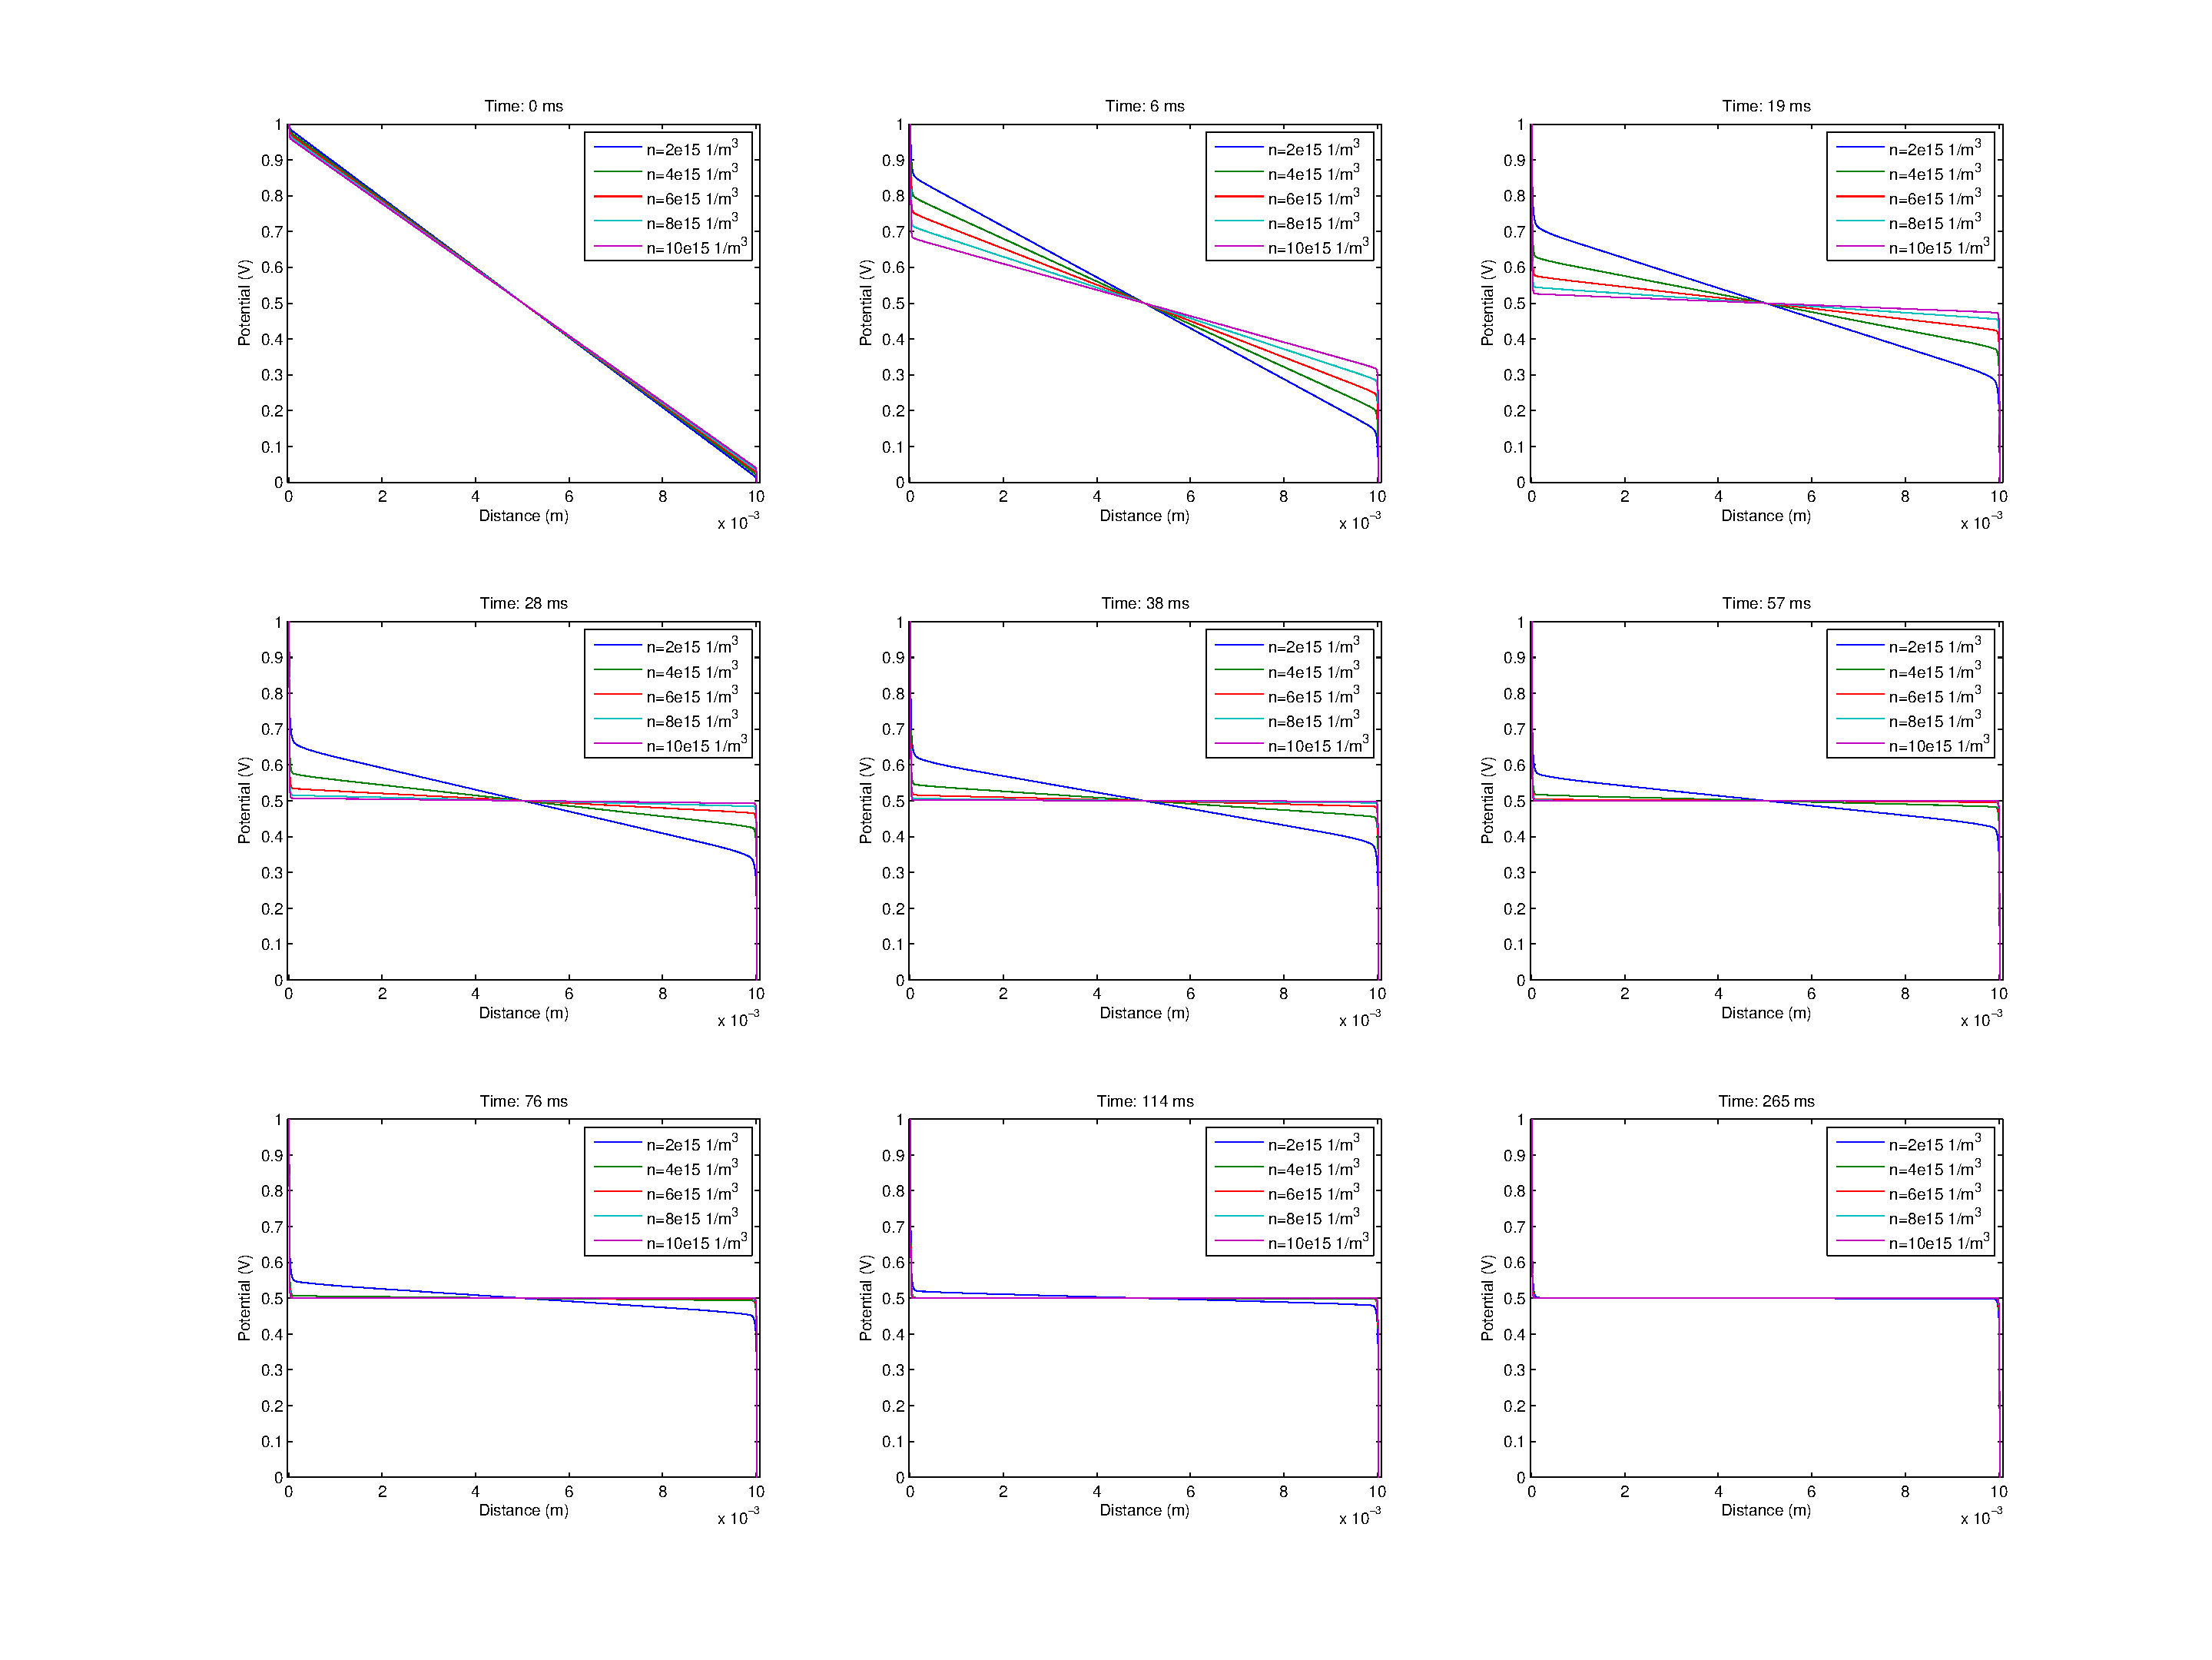
\includegraphics[scale=0.40]{Ex1V_Time}
\caption{Potential distribution in electrolyte over time} 
\label{ElectrolyteV}
\end{figure}
\end{landscape}

 
\begin{landscape}
\begin{figure}[!htp]
\centering
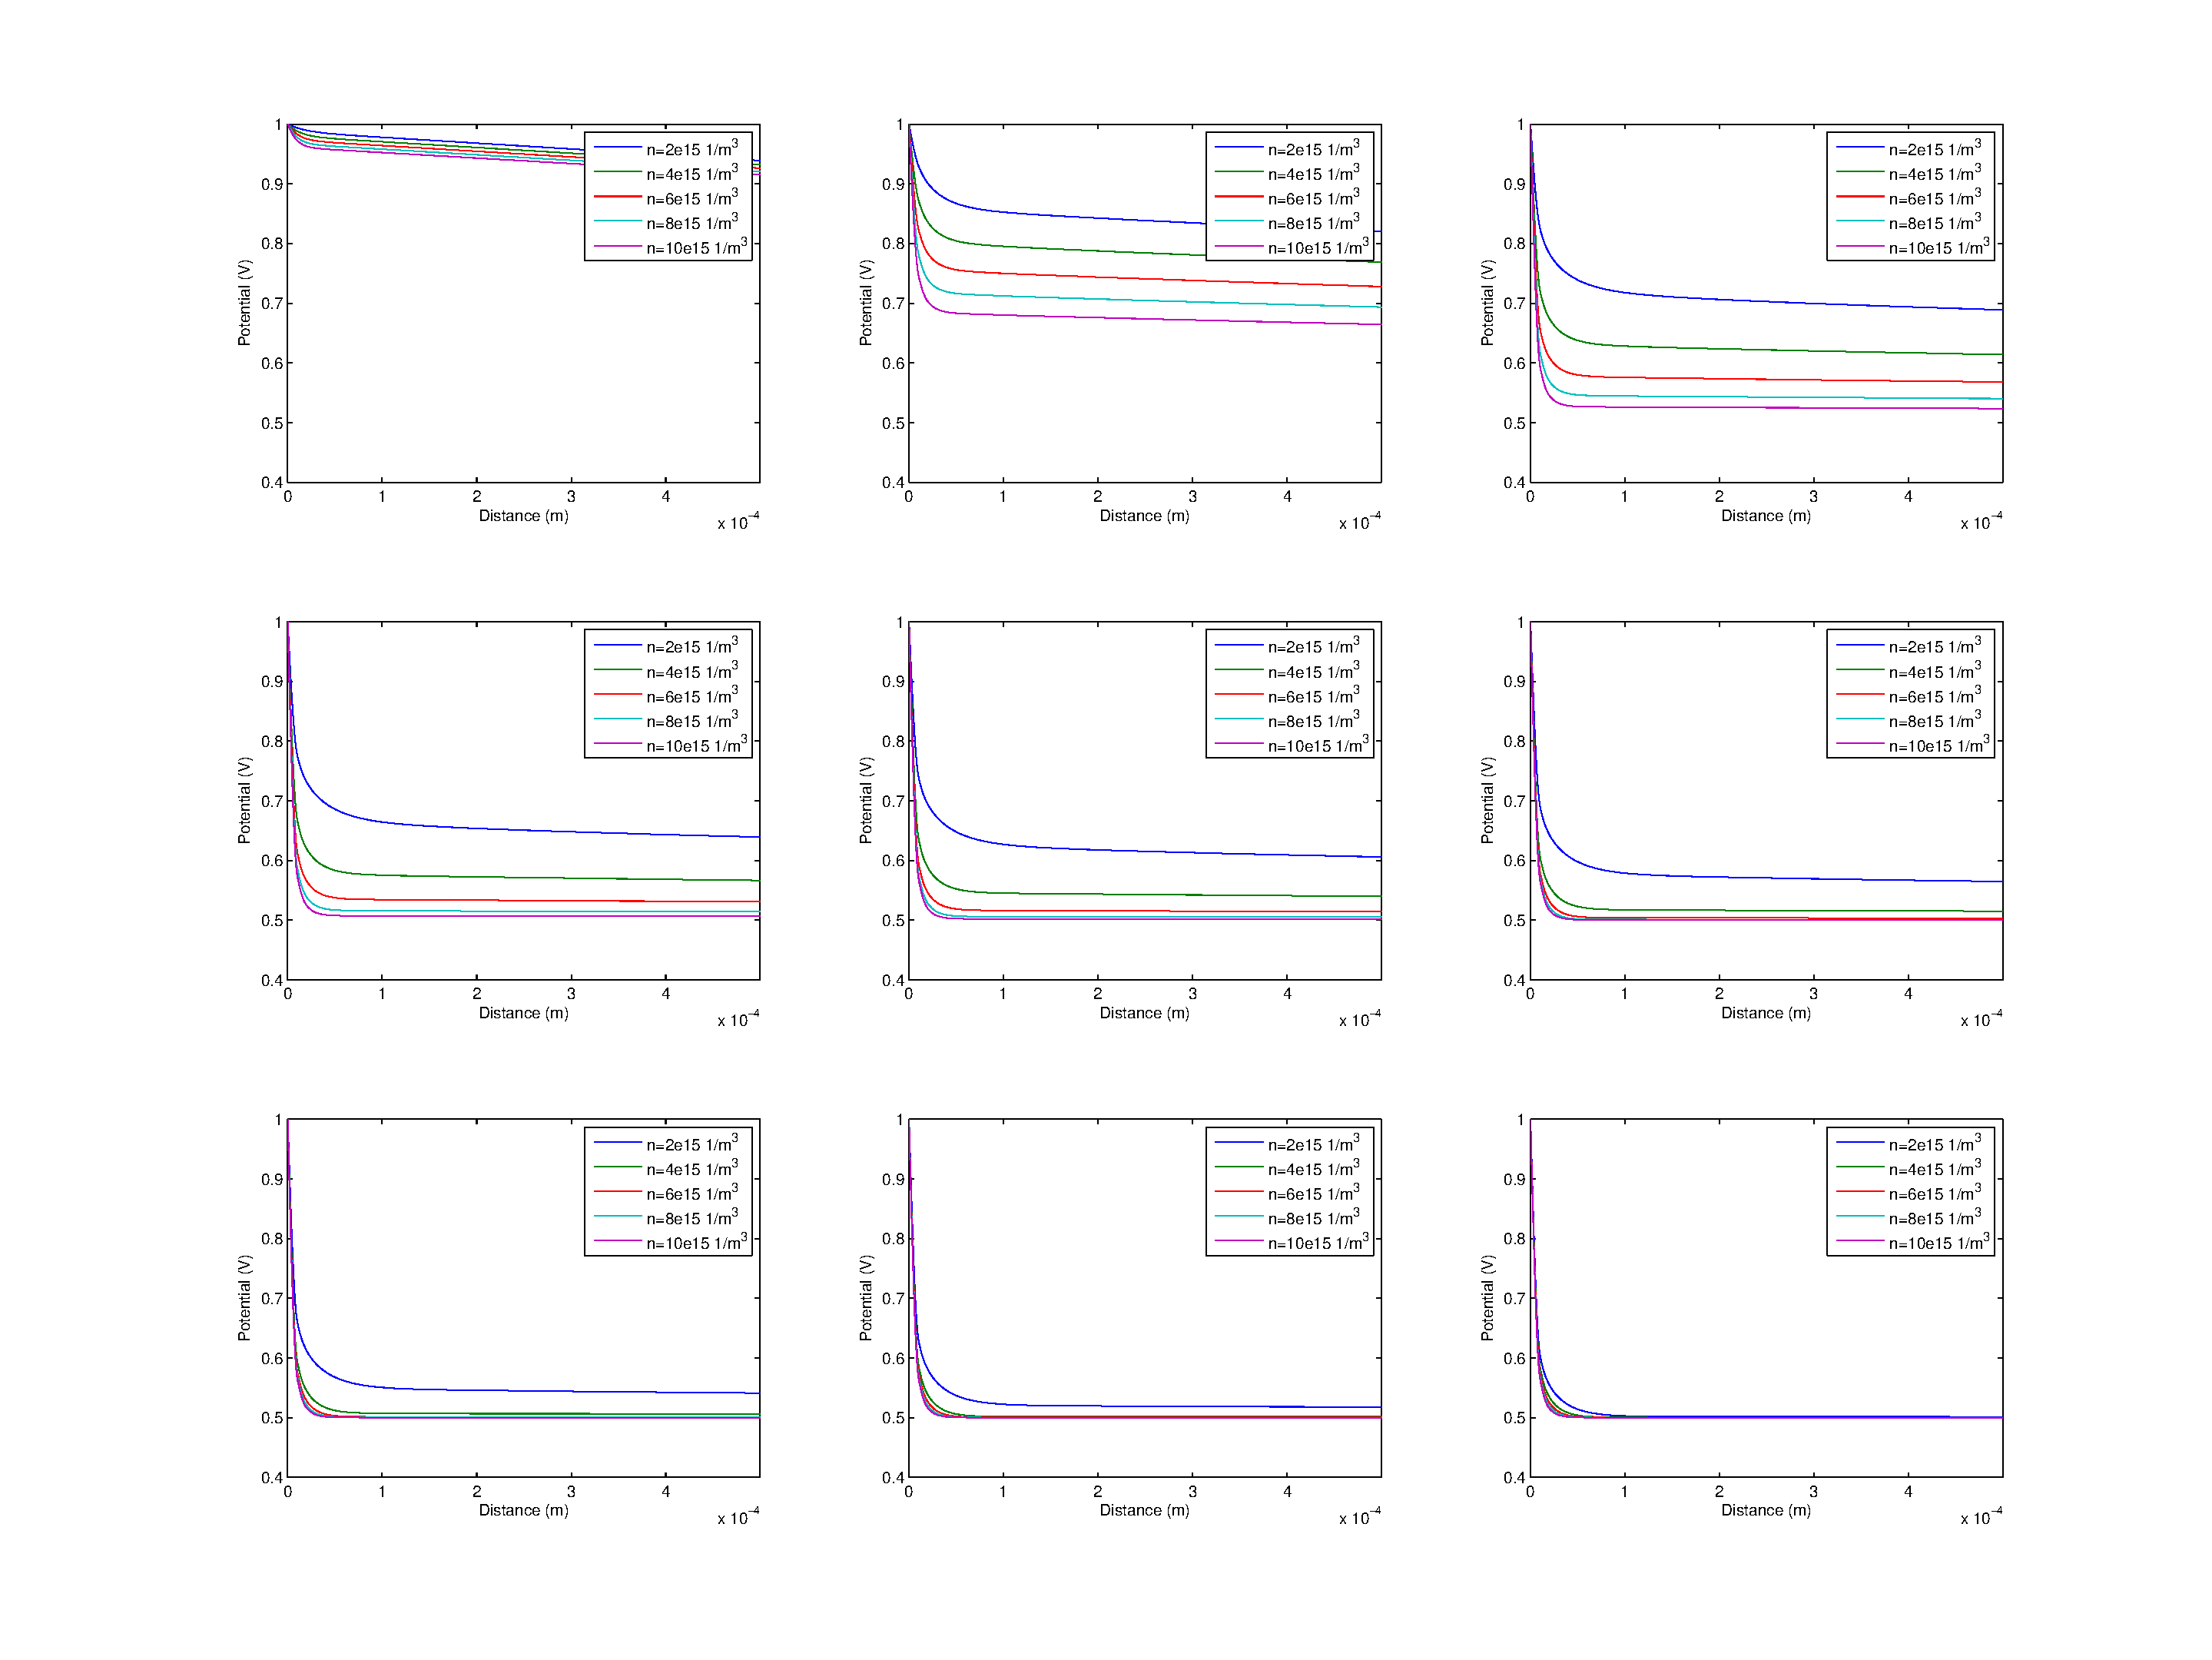
\includegraphics[scale=0.40]{Ex1V_Time2}
\caption{Potential distribution on the left wall of the electrolyte over time} 
\label{ElectrolyteV2}
\end{figure}
\end{landscape}

\clearpage
\subsection{1-D Horizontal Memristor (Cross Section 2)}

Cross section 2 from figure \ref{MemStc} has the most crucial elements of the memristor but its simulation in 1-D is not as straight forward as the simulation of the electrolyte. Horizontal cross section through the PEDOT does not include the vertical movement of lithium. Without this effect PEDOT is just a regular conductor with a uniform current density. In order to overcome this problem a generation/recombination term for lithium ions, calculated at every time step, was added to capture the vertical movement in addition to regular drift diffusion equations which represents the horizontal movement. This generation/recombination term can be represented as a current source with a resistor connected to every node (figure \ref{MemStc15}). 

The lithium source has two different terms, one for drift and another one for diffusion. It was assumed that the concentration of lithium was always constant in the electrolyte. This way the vertical diffusion current density can be calculated using the difference between the lithium density in PEDOT and electrolyte. For the diffusion term an electric field has to be estimated between the PEDOT and the electrolyte. First the potential of the electrolyte was assumed to be half of the net applied potential. Then an electric field is calculated using the electrolyte and the potential of the PEDOT at different positions.
  
\begin{figure}[!htp]
\centering
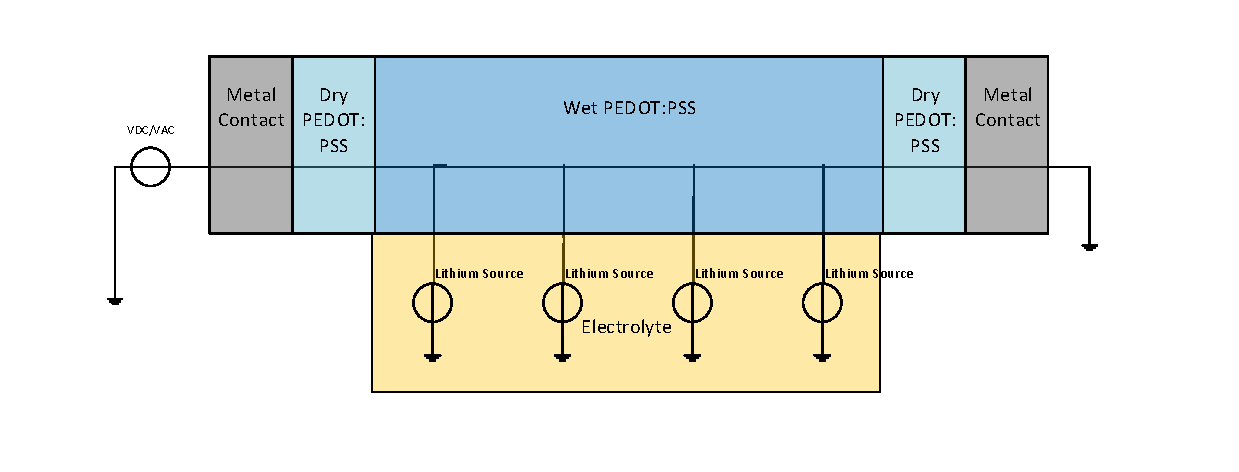
\includegraphics[scale=0.74]{1DMem}
\caption{1.5-D Memristor Structure} 
\label{MemStc15}
\end{figure}


\begin{landscape}
\begin{figure}[!htp]
\centering
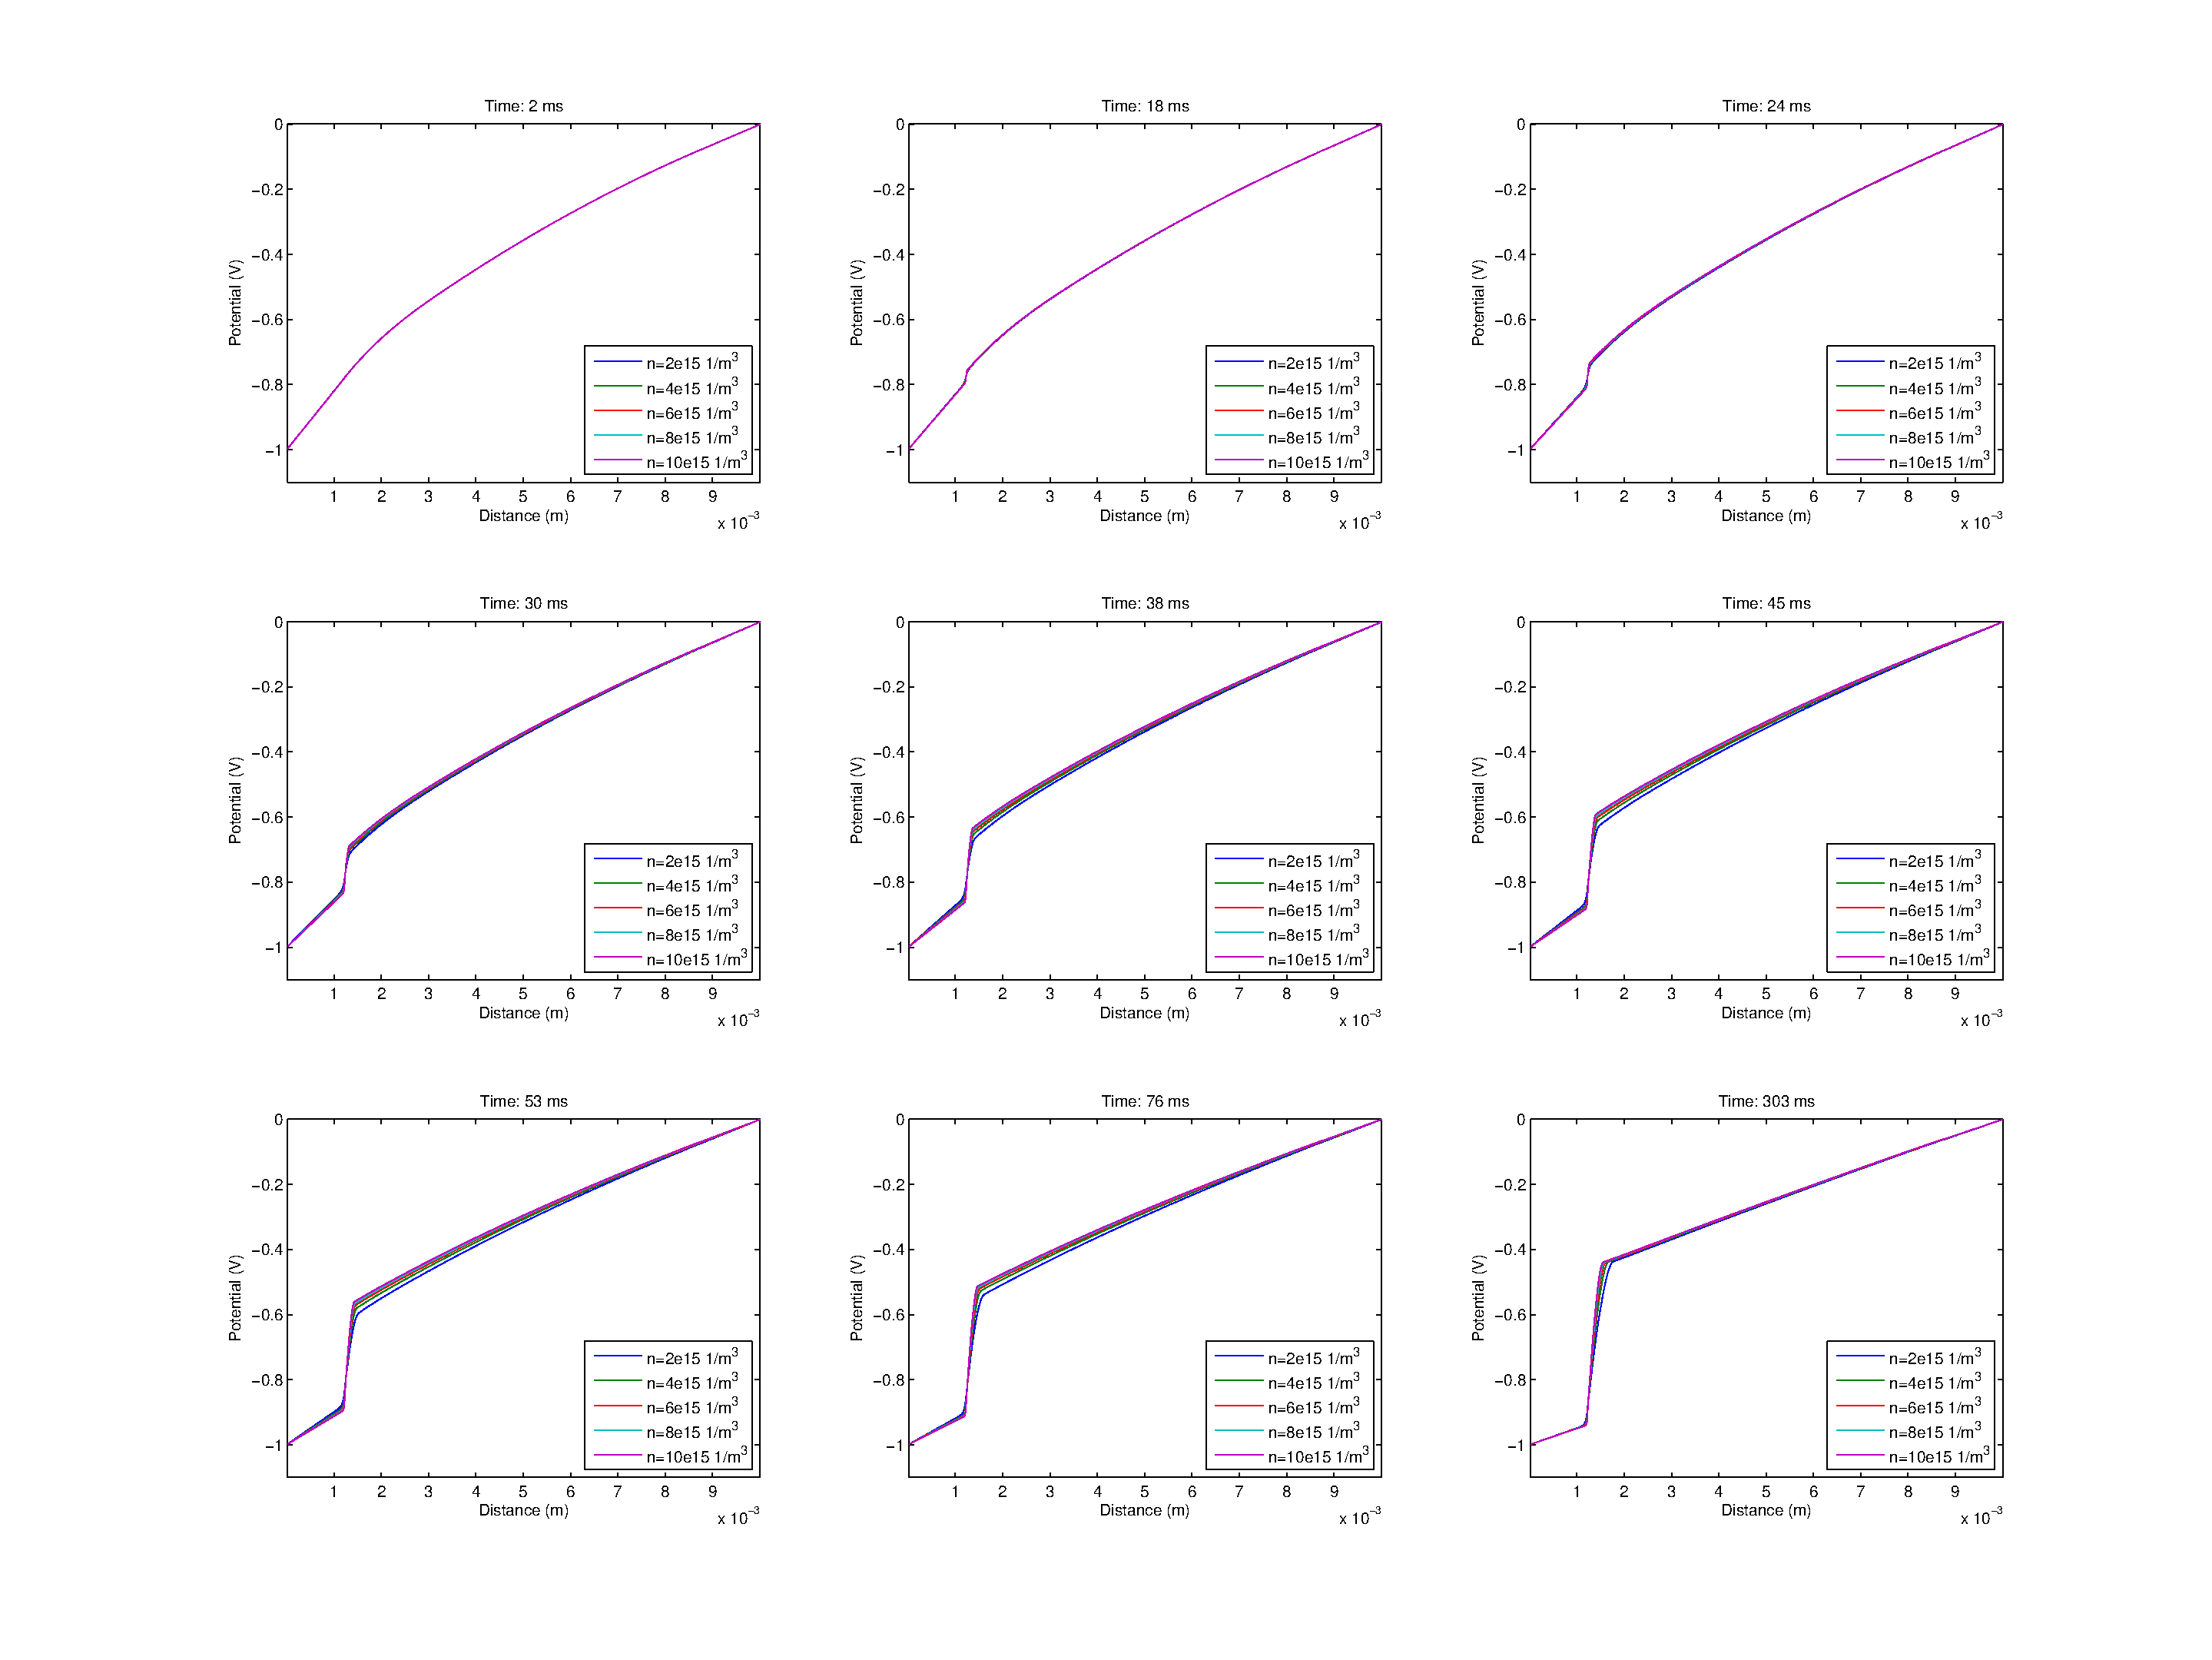
\includegraphics[scale=0.40]{Ex5V_Time1}
\caption{1-D Memristor potential distribution over time} 
\label{}
\end{figure}
\end{landscape}


\begin{landscape}
\begin{figure}[!htp]
\centering
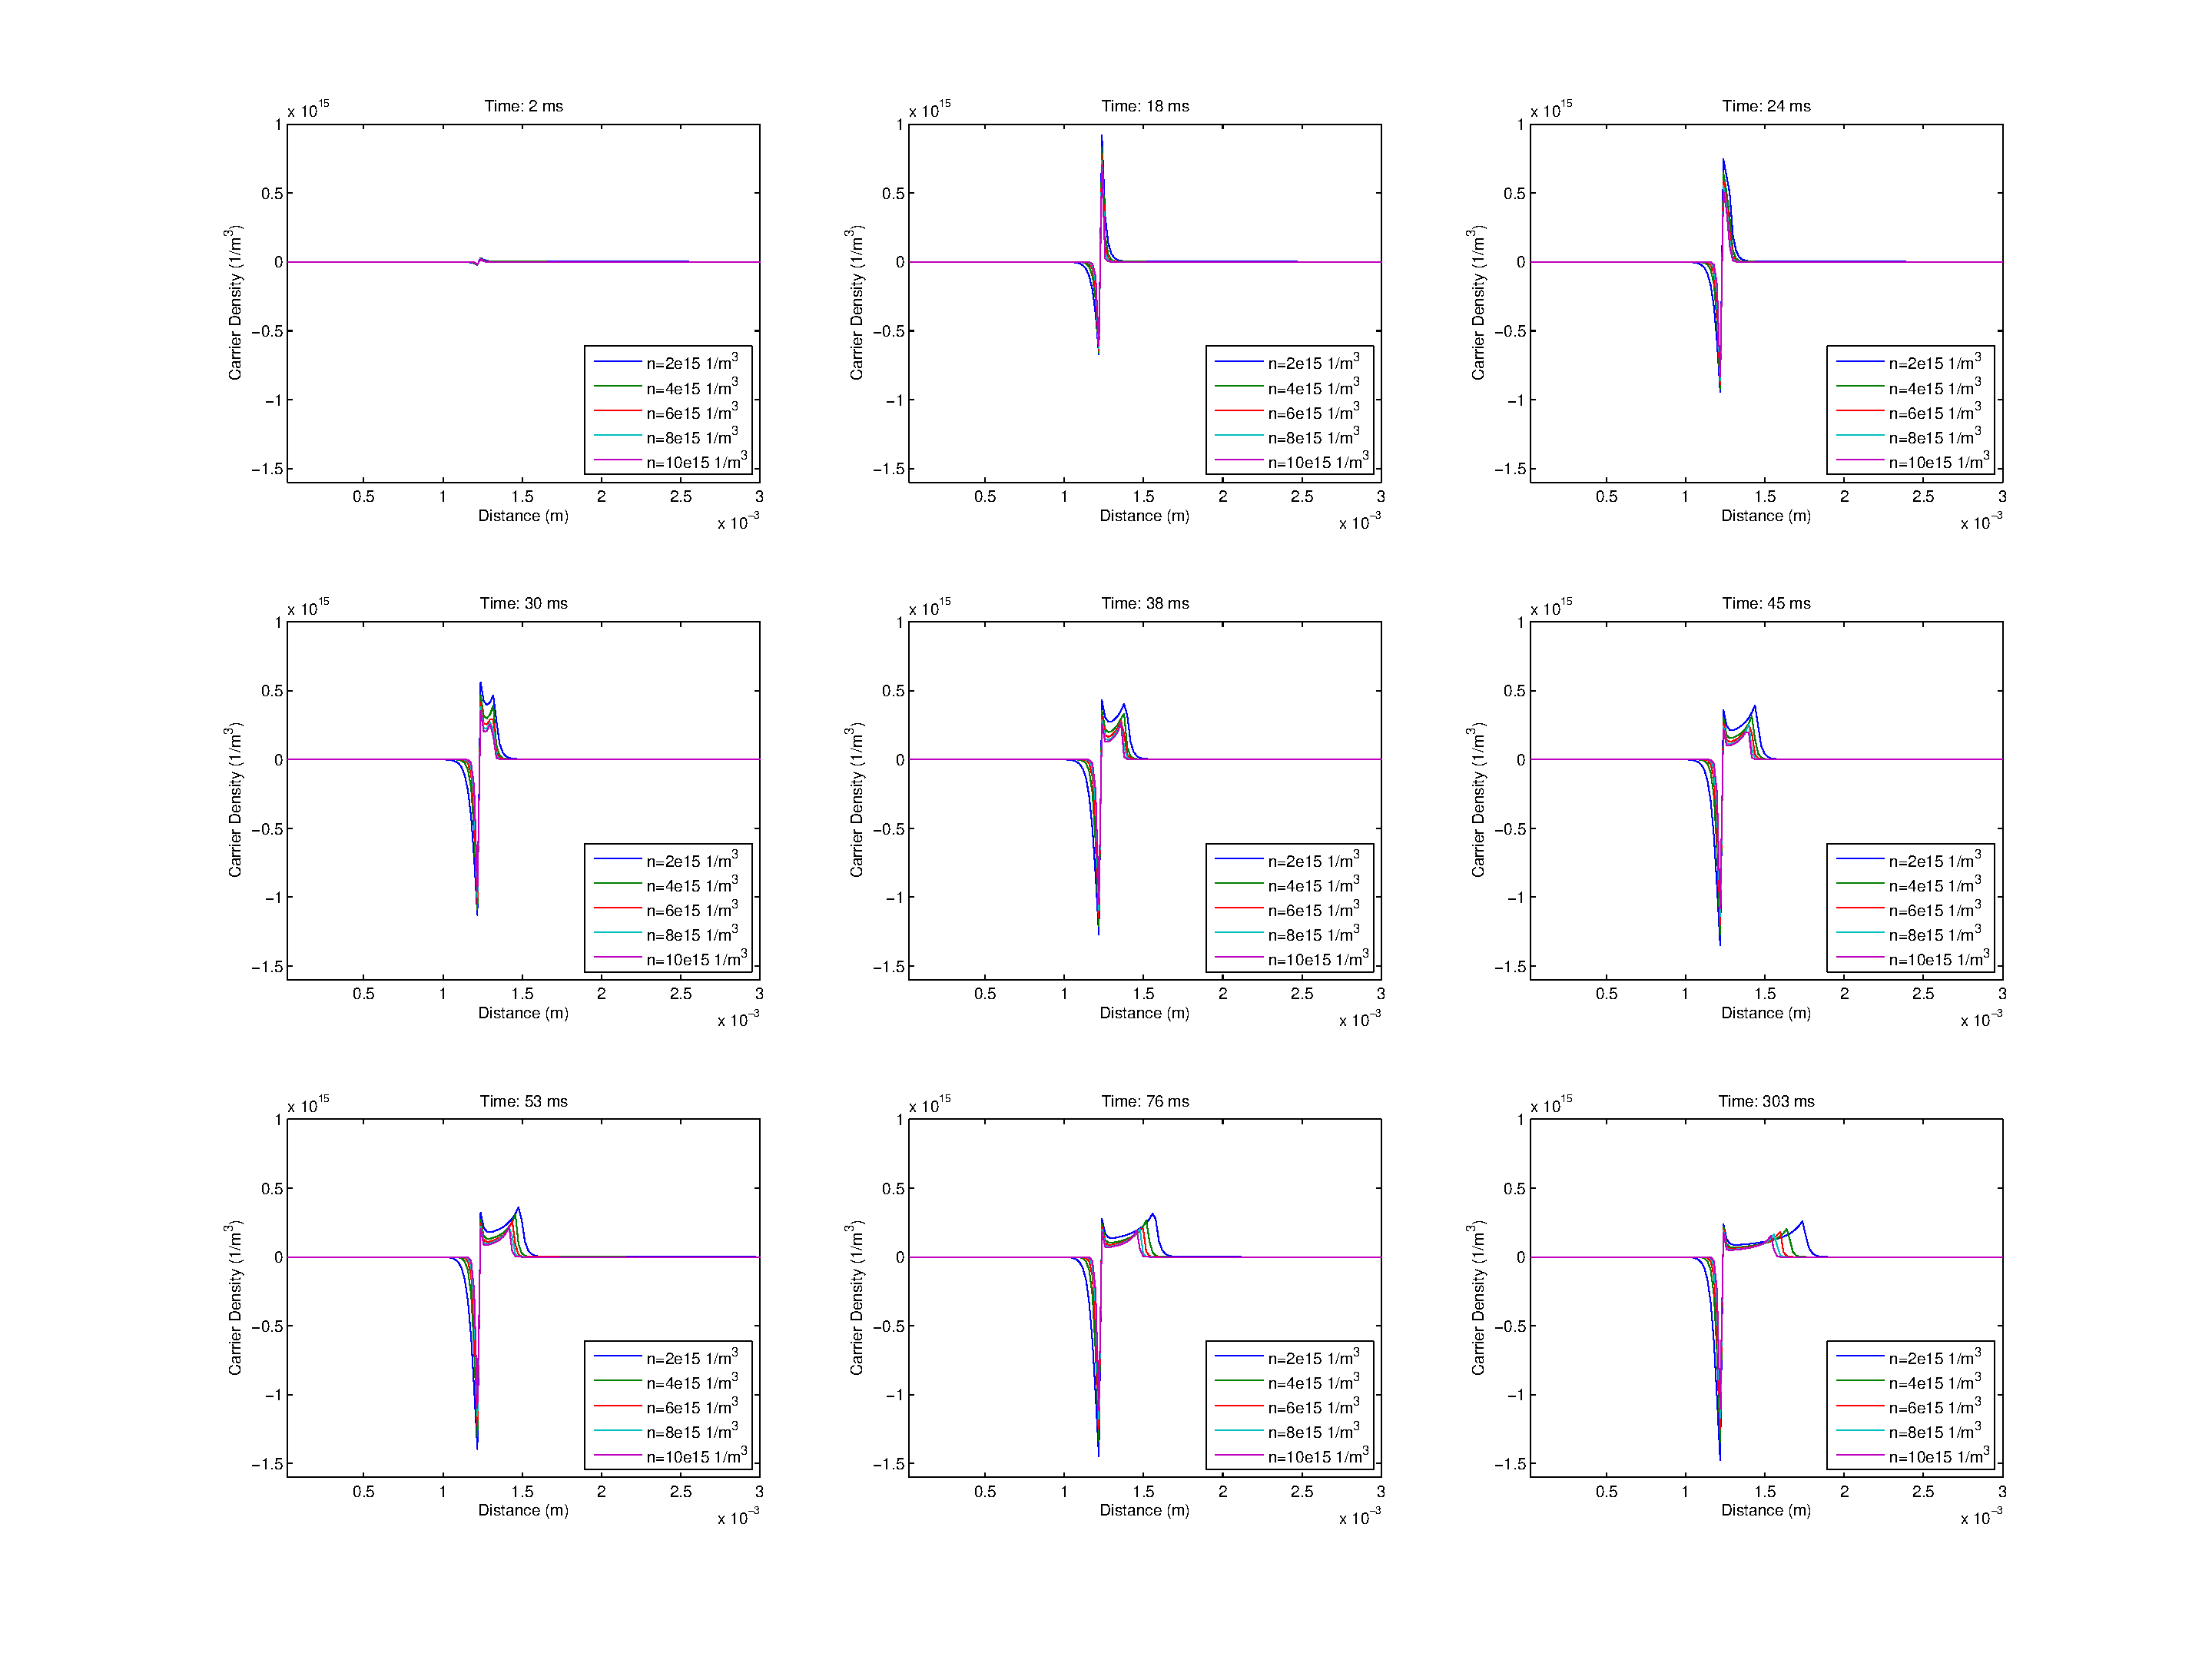
\includegraphics[scale=0.40]{Ex5NetQ_Time1}
\caption{Normalized net charge density distribution over time} 
\label{}
\end{figure}
\end{landscape}


\begin{landscape}
\begin{figure}[!htp]
\centering
\includegraphics[scale=0.40]{Ex5Np_Time1}
\caption{Normalized lithium density distribution over time} 
\label{}
\end{figure}
\end{landscape}


\begin{landscape}
\begin{figure}[!htp]
\centering
\includegraphics[scale=0.40]{Ex5p_Time1}
\caption{Normalized hole density distribution over time} 
\label{}
\end{figure}
\end{landscape}

\begin{landscape}
\begin{figure}[!htp]
\centering
\includegraphics[scale=0.40]{Ex5pNp_Time1}
\caption{Lithium and hole density distribution over time} 
\label{}
\end{figure}
\end{landscape}



\begin{figure}[!htp]
\centering
\includegraphics[scale=0.60]{Ex5Bowtie}
\caption{Normalized Current vs. potential} 
\label{}
\end{figure}

\begin{figure}[!htp]
\centering
\includegraphics[scale=0.60]{Ex5Current}
\caption{Normalized current over time} 
\label{}
\end{figure}



\clearpage
\subsection{PEDOT:PSS with Notch (Cross Section 2)}


\begin{landscape}
\begin{figure}[!htp]
\centering
\includegraphics[scale=0.40]{Ex5V_Notch_Time1}
\caption{Notched memristor potential distribution over time} 
\label{}
\end{figure}
\end{landscape}



\begin{landscape}
\begin{figure}[!htp]
\centering
\includegraphics[scale=0.40]{Ex5Hole_Notch_Time1}
\caption{Normalized hole distribution over time} 
\label{}
\end{figure}
\end{landscape}


\begin{landscape}
\begin{figure}[!htp]
\centering
\includegraphics[scale=0.40]{Ex5Li_Notch_Time1}
\caption{Normalized lithium distribution over time} 
\label{}
\end{figure}
\end{landscape}


\begin{landscape}
\begin{figure}[!htp]
\centering
\includegraphics[scale=0.40]{Ex5Lip_Notch_Time1}
\caption{Lithium and hole distribution over time} 
\label{}
\end{figure}
\end{landscape}


\clearpage
\subsection{Electrolyte/PEDOT Interface (Cross Section 3) }

\begin{landscape}
\begin{figure}[!htp]
\centering
\includegraphics[scale=0.40]{Ex4V_Time}
\caption{Electrolyte/PEDOT interface potential distribution over time} 
\label{}
\end{figure}
\end{landscape}


\begin{landscape}
\begin{figure}[!htp]
\centering
\includegraphics[scale=0.40]{Ex4Np_Time}
\caption{Normalized lithium distribution over time} 
\label{}
\end{figure}
\end{landscape}

\begin{landscape}
\begin{figure}[!htp]
\centering
\includegraphics[scale=0.40]{Ex4p_Time}
\caption{Normalized hole distribution over time} 
\label{}
\end{figure}
\end{landscape}

\begin{landscape}
\begin{figure}[!htp]
\centering
\includegraphics[scale=0.40]{Ex4pNp_Time}
\caption{Lithium and hole distribution over time} 
\label{}
\end{figure}
\end{landscape}






%1-D Vertical Medium and high concentration (hole freeze,# of holes over time)
%1-D Horizontal medium and high concentration (Add memristor pictures,hole freeze,# of holes over time)
 
% Chapter Template

\chapter{Memristor Simulation} % Main chapter title

\label{Chapter6} % Change X to a consecutive number; for referencing this chapter elsewhere, use \ref{ChapterX}

\lhead{Chapter 6. \emph{Memristor Simulation}} % Change X to a consecutive number; this is for the header on each page - perhaps a shortened title

\section{2-D Memristor Model}


After creating a method to solve drift diffusion equations using finite difference in chapter 4 and testing it in chapter 5 we can now simulate an actual memristor. The most basic memristor structure consists of a rectangular strip of PEDOT with metal/carbon contacts on both sides. On top of the strip there is a drop of electrolyte solution. In order to be able to simulate the memristor we first need to determine boundary conditions and values, initial conditions and physical constans for this device.

We have two different materials and three charge carriers that are important for this problem. The drop of electrolyte has lithium and perchlorate ions and PEDOT has holes and electrons. All the carriers are not free to move everywhere. Due to PEDOT's conduction mechanism the electrons are fixed in place and holes are mobile. Also because of PEDOT's chemistry only lithium is allowed to move in so perchlorate ions always stay in the electrolyte. When a lithium ion moves into the PEDOT, through drift or diffusion, it replaces a hole. This replacement reduces the number of available holes in the PEDOT and increases its resistance. 

For the initial concentration of ions in the electrolyte we have assumed that there is no net charge and everything is uniformly distributed. Similar to electrolyte PEDOT has no net charge. All the electrons and holes are uniformly distributed and in equilibrium. Boundary conditions for all species are no flow boundary conditions with the exception of holes which can leave PEDOT through the contacts. On the contacts zero net charge is always conserved through the movement of holes in and out of the device. Lithium atoms can move between PEDOT and the electrolite but they cannot go through the contacts. Also there is a limit on the amount of lithium PEDOT can accept. Once all the holes have been replaced lithium ions cannot go into the PEDOT anymore.

The difference between the thickness of the PEDOT and electrolyte makes the simulation very difficult using uniform meshing. The thickness of the electrolyte was shortened by assuming that the amount of charge in the electrolyte is very large and more than enough to saturate PEDOT with lithium ions. Very thick electrolyte was replaced by a thinner one and the top part assumed to be an infinite source/drain for ions.

The contacts have constant potential so they have dirichlet boundary conditions. There were no constraints for the edges of the simulation domain so the potential was set to float using Neumann boundary condition.

Another important aspect of this device is the change in mobility between different materials. Lithium ions move very slowly when they get intercalated into the PEDOT. Also the regions of PEDOT that are in contact with the electrolite (wet region) has higher mobility for lithium compared to the regions that are not in contact (dry region).

\clearpage
\subsection{Intercalation of Lithium Ions}

The following series of simulations were done to study how adding various effects changes the intercalation of lithium ions into PEDOT. We have six different scenarios with increasing complexity. All the simulations start at same initial conditions shown in figure \ref{61101}. The ions are all in the electrolyte and they are uniformly distributed. All the holes and electrons are in PEDOT and they are also uniformly distributed. All the positive charges in the system are balanced by negative charges. For the following six simulations the change of mobility between wet and dry regions are abrupt so lithium cannot move past the wet region of the PEDOT.

\begin{figure}[!htp]
\centering
\includegraphics[scale=0.8]{61101}
\caption{Initial distribution of holes, electrons, lithium and perchlorate } 
\label{61101}
\end{figure}

The result of the first simulation is shown in figure \ref{NnNpp61101}. In this case the equations are assumed to be decoupled and there is no applied potential at the contacts. This means that there is no electric field and the only force acting on the particles is diffusion. Perchlorate ions and holes have nowhere to diffuse into so their concentrations stay constant. However, lithium ions diffuse freely into the PEDOT until overall density is uniform since there is no limit on its density. 

\begin{figure}[!htp]
\centering
\includegraphics[scale=0.8]{NnNpp61101}
\caption{Particle distribution at steady state without any applied potential or density limit. Equations are decoupled} 
\label{NnNpp61101}
\end{figure}

In this second example shown in figure \ref{NnNpp61102} we kept all the conditions the same but applied a constant potential at the contacts. The electric field pulls lithium and perchlorate ions towards opposite sides. Lithium atoms drift and diffuse into the PEDOT and perchlorate ions stay in the electrolyte as expected. PEDOT just behaves like a regular resistor and holes uniformly flow in and out of the device.

\begin{figure}[!htp]
\centering
\includegraphics[scale=0.75]{NnNpp61102}
\caption{Particle distribution at steady state with applied potential and without density limit. Equations are decoupled} 
\label{NnNpp61102}
\end{figure}

A limit for lithium was added for the last simulation without coupled equations. If we compare figure \ref{NnNpp61102} and \ref{NnNpp61103} we can clearly see the difference in lithium density in PEDOT as it gets uniformly distributed instead of exponentially collecting on one side. Lithium still has no effect on holes since the electric field due to charged particles are ignored.

For the last three examples we will be going over the same simulations by taking coupling into account. With the addition of coupling between Poisson's equation and drift diffusion equations, the system of particles will always try to stay as charge neutral as possible. 

 
\begin{figure}[!htp]
\centering
\includegraphics[scale=0.76]{NnNpp61103}
\caption{Particle distribution at steady state with applied potential and density limit. Equations are decoupled} 
\label{NnNpp61103}
\end{figure}

Figure \ref{NnNpp61104} is good example illustrating this effect since the only drift force pushing the particles are self generated. Lithium ions diffuse into PEDOT leaving a net negative charge near the interface which pulls them back into the electrolyte. Now since there is an accumulation of positive charge inside the PEDOT perchlorate ions move towards the interface. At the same time holes are being pushed out from PEDOT and they are slowly getting replaced by lithium ions. Figure \ref{NnNpp61104} clearly shows that there is a lack of holes where lithium ions have diffused in.

\begin{figure}[!htp]
\centering
\includegraphics[scale=0.77]{NnNpp61104}
\caption{Particle distribution at steady state without any applied potential or density limit. Equations are coupled} 
\label{NnNpp61104}
\end{figure}

As before adding a potential to the contacts separates positive and negative ions. This time hey will separate until the electric field is canceled out. In figure \ref{NnNpp61105} we can see the negative charges in the electrolyte holding most lithium ions from moving into the PEDOT. Also as they move into the PEDOT the electric field gets weaker. So compared to the case without coupling (figure \ref{NnNpp61102}) there are less lithium ions in the PEDOT. On the right side of the PEDOT we can see a strip of missing holes due to the migration of lithium. We can also see holes accumulating at the interface on the left side due to the increased amount of perchlorate ions right across the interface.

\begin{figure}[!htp]
\centering
\includegraphics[scale=0.71]{NnNpp61105}
\caption{Particle distribution at steady state with applied potential and without density limit. Equations are coupled} 
\label{NnNpp61105}
\end{figure}

In the last example (figure \ref{NnNpp61106}) the addition of the density limit flattens out the accumulation of lithium ions in the PEDOT. We can see that holes are getting replaced by lithium on a larger area since its accumulation is not as concentrated at the edge. The accumulation of holes due to perchlorate ions across the interface does not get affected by this change.

\begin{figure}[!htp]
\centering
\includegraphics[scale=0.71]{NnNpp61106}
\caption{Particle distribution at steady state with applied potential and without density limit. Equations are decoupled} 
\label{NnNpp61106}
\end{figure}

Finally we can look at how the electric field looks at steady state. We see an electric field in figure \ref{V61102}.a created by the excess of positive charge in the PEDOT due to the diffusion of lithium. Even though there is an electric field in this simulation, its magnitude is so small that it does not have any impact on the movement of the charge carriers. In the last two figures at the top row (figure \ref{V61102}.b and \ref{V61102}.c) we can see the uniform electric field created by the potential applied at the contacts. Since the equations are decoupled the electric field does not get affected by the redistribution of charge. In figure \ref{V61102}.d most of the electric field is generated due to the diffusion of lithium into PEDOT. Net positive charge in the PEDOT, under the electrolyte, creates an outward electric field. 

The effects of coupling in the potential can be easily seen by comparing figure \ref{V61102}.b and \ref{V61102}.e. In the electrolyte charges separate and cancel the electic field. In the PEDOT there is a very high electric field at the interface between wet and dry regions since lithium ions cannot travel into the dry region. The limitation of lithium density in the PEDOT decreases the sharpness of the change in charge density therefore the electric field changes over a slightly longer distance. 
\begin{landscape}
\begin{figure}[!htp]
\centering
\includegraphics[scale=0.60]{V61102}
\caption{Potential and Electric Field in Steady State} 
\label{V61102}
\end{figure}
\end{landscape}


\clearpage
\section{Simulation vs. Experimental Results}

\subsection{Single Channel Memristor}

In this section we will be looking into the transient simulation of a single channel memristor which is very similar to the last simulation of the previous section. Drift diffusion and Poisson's equations are coupled and lithium density is limited in PEDOT. In addition, the mobility of lithium is now gradually changing between wet and dry regions. This way lithium ions can penetrate the dry region but they cannot move too far. For transient simulation a constant potential has been applied until steady state. Once the memristor reached steady state the polarity of the potential has been switched and the simulation was run until it reached steady state. 

\begin{figure}[!htp]
\centering
\includegraphics[scale=0.65]{Cd_Li_p_1}
\caption{Particle distribution right after the simulation has started} 
\label{Cd_Li_p_1}
\end{figure}

Following graph (\ref{Cd_Li_p_1}) shows the distribution of charged particles right after the simulation has started using initial conditions described in figure \ref{61101}. We can see that perchlorate ions quickly redistribute and pile up at the bottom right corner of the electrolyte. Lithium ions drift and diffuse into the PEDOT and move as far as they can towards the contact but they cannot reach it due to the decreased mobility in the dry region. Holes accumulate right on the interface between PEDOT and electrolyte in response to perchlorate accumulation. We can also see holes being pushed out on the left side due to the migration of lithium into PEDOT. 

At steady state we can see lithium accumulating on the left side of PEDOT and creating an area with very low hole density therefore high resistance (figure \ref{Cd_Li_p_2}). 

\begin{figure}[!htp]
\centering
\includegraphics[scale=0.65]{Cd_Li_p_2}
\caption{Particle distribution at steady state} 
\label{Cd_Li_p_2}
\end{figure}

After the potential has been flipped (figure \ref{Cd_Li_p_3}) we can see that some lithium that got into the dry region of the PEDOT does not leave right away due to low mobility. Also, the change in potential forces lithium ions to accumulate on the right side of PEDOT.
 
\begin{figure}[!htp]
\centering
\includegraphics[scale=0.65]{Cd_Li_p_3}
\caption{Particle distribution after the potential has been changed} 
\label{Cd_Li_p_3}
\end{figure}

Finally once everything reaches steady state again almost all of the lithium ions that ware stuck in the dry region of PEDOT moved away. The final distribution for all particles looks like a mirror image of the situation with opposite potential (figure \ref{Cd_Li_p_2}). This is expected since the device is completely symmetrical.

\begin{figure}[!htp]
\centering
\includegraphics[scale=0.65]{Cd_Li_p_4}
\caption{Particle distribution at steady state after the potential has been changed} 
\label{Cd_Li_p_4}
\end{figure}

The next five graphs show the evolution of the potential and the electric field over time. The snapshots were taken at the same time as the ones for charged particles. The first figure (\ref{EV_0}) shows the initial potential distribution. At te second figure (\ref{EV_1}) We can see the large electric field between the PEDOT and electrolyte created by the accumulation of holes and perchlorate on both sides. Additionally the electric field inside the electrolyte is getting canceled out due to separation of charge.

\begin{figure}[!htp]
\centering
\includegraphics[scale=0.77]{EV_0}
\caption{Electric field and potential distribution before any movement of charge} 
\label{EV_0}
\end{figure}

\begin{figure}[!htp]
\centering
\includegraphics[scale=0.75]{EV_1}
\caption{Electric field and potential distribution right after the simulation has started} 
\label{EV_1}
\end{figure}

At steady state there is almost no electric field inside the electrolyte (figure \ref{EV_2}). Most of the electric field inside PEDOT is also canceled out by the accumulation of lithium on the left side. Almost all the electric field is concentrated around the region where lithium accumulates and forces holes out. Since the electrons are fixed in place, when holes move out they leave behind an exposed negative charge in the dry region. This strengthens the electric field even further.

\begin{figure}[!htp]
\centering
\includegraphics[scale=0.75]{EV_2}
\caption{Electric field and potential distribution at steady state} 
\label{EV_2}
\end{figure}

As soon as the potential is switched we see a change in the electric field between PEDOT and electrolyte (figure \ref{EV_3}). The electric field created by lithium on the left side of the PEDOT quickly disappears. The dark spot on the left side of PEDOT is due to lithium taking time to move towards the other side.

\begin{figure}[!htp]
\centering
\includegraphics[scale=0.75]{EV_3}
\caption{Electric field and potential distribution right after the applied potential has been changed} 
\label{EV_3}
\end{figure}

At steady state the potential distributions of \ref{EV_2} and \ref{EV_4} are mirror images of each other except the polarity of the applied potential at the contacts are opposite. This is not unexpected since charge particle distributions had the exact same behavior. 

\begin{figure}[!htp]
\centering
\includegraphics[scale=0.75]{EV_4}
\caption{Electric field and potential distribution at steady state after the applied potential has been changed} 
\label{EV_4}
\end{figure}

Figures \ref{Edge_1} to \ref{Edge_6} show the horizontal cross section of lithium around the wet dry/interface of PEDOT. The figures on the left side are simulation results and the figures on the right side are experimental results. Unfortunately we did not have any means of directly measuring the lithium density. The closest option to measuring lithium density in PEDOT was to capture the blue coloration of PEDOT when it interacts with lithium. This was done by recording the video of the experiment as it goes through different stages. Afterwards, the images were filtered and processed to show high values for blue and low values for other colors. 

The figure below shows the distribution of lithium right before the potential is flipped. We can see , from both simulation and experimental results, that as time progresses lithium moves towards the opposite side of the device and leaves behind a trail where mobility is very low. 

Another phenomenon that was observed in the experiment was the change in lithium penetration into dry PEDOT due to increased applied potential. The last figure in this chapter (\ref{EdgeV}) shows the maximum distance lithium travels into the dry region of PEDOT with increasing potential at the contacts. Both simulation and the experiment follow a similar trend but they deviate at higher voltages. There could be a few reasons for this discrepancy. First of all it is very hard to get an exact function for the change between wet and dry regions through experimentation so any function used to model this gradual change had to be optimized by trial and error. Since the simulation for every data point takes a very long time to run, it is very difficult to find a general function that fits all the data points. Also the grid used to simulate this problem was quite coarse so there were only a few points to represent the change between two regions.

\begin{figure}[!htp]
\centering
\includegraphics[scale=0.75]{Edge_1}
\caption{Lithium movement at wet/dry interface} 
\label{Edge_1}
\end{figure}

\begin{figure}[!htp]
\centering
\includegraphics[scale=0.75]{Edge_2}
\caption{Lithium movement at wet/dry interface} 
\label{Edge_2}
\end{figure}

\begin{figure}[!htp]
\centering
\includegraphics[scale=0.75]{Edge_3}
\caption{Lithium movement at wet/dry interface} 
\label{Edge_3}
\end{figure}


\begin{figure}[!htp]
\centering
\includegraphics[scale=0.75]{Edge_4}
\caption{Lithium movement at wet/dry interface} 
\label{Edge_4}
\end{figure}

\begin{figure}[!htp]
\centering
\includegraphics[scale=0.75]{Edge_5}
\caption{Lithium movement at wet/dry interface} 
\label{Edge_5}
\end{figure}

\begin{figure}[!htp]
\centering
\includegraphics[scale=0.75]{Edge_6}
\caption{Lithium movement at wet/dry interface} 
\label{Edge_6}
\end{figure}

\begin{figure}[!htp]
\centering
\includegraphics[scale=0.75]{EdgeV}
\caption{Penetration of lithium into dry PEDOT} 
\label{EdgeV}
\end{figure}

\clearpage
\subsection{Noteched PEDOT}

In this section we will be looking at a structure which is very similar to the single channel memristor. All the boundary conditions and initial values are the same except this time there is a notch in the PEDOT (figure \ref{NCd_Li_p_0}). So there is no hole current through the device and lithium cannot migrate into the notch. The device itself has very limited practical use but the experimental results are very suitable to test our numerical model. 

\begin{figure}[!htp]
\centering
\includegraphics[scale=0.9]{NCd_Li_p_0}
\caption{Initial hole, electron, perchlorate and lithium distribution for a notched memristor} 
\label{NCd_Li_p_0}
\end{figure}

The notch in the PEDOT is sandwiched between two conductive parts. This is analogous to having a simple circuit with two low and one high resistance in series. Based on this analogy we can see that almost all the potential drop is going to be on the notch. One side of the PEDOT will have a low potential and the other side will have a high potential. In figure \ref{NCD_Li_p_1} we can see lithium slowly moving towards the negative side of the PEDOT. At the same time perchlorate is starting to accumulate on the positive side. We can also see a significant hole accumulation inside PEDOT right before the notch. 

\begin{figure}[!htp]
\centering
\includegraphics[scale=0.7]{NCd_Li_p_1}
\caption{Particle distribution shortly after the simulation has started} 
\label{NCD_Li_p_1}
\end{figure}

As time goes by more lithium is pushed away from the positive side of the PEDOT and pulled into the negative side (figure \ref{NCD_Li_p_2}). The here is a noticeable lack of lithium on the side with positive contact at the electrolyte/PEDOT interface. While lithium is pulled into the PEDOT holes are being pushed away. Holes also accumulate at the surface of the PEDOT due to accumulation of perchlorate right across the interface.

\begin{figure}[!htp]
\centering
\includegraphics[scale=0.7]{NCd_Li_p_2}
\caption{Particle distribution before steady state} 
\label{NCD_Li_p_2}
\end{figure}

At steady state we can see that lithium density in PEDOT is uniform and at its maximum value (\ref{NCd_Li_p_3}). At the same area we can see the lack of holes due to migration of lithium.
 
\begin{figure}[!htp]
\centering
\includegraphics[scale=0.7]{NCd_Li_p_3}
\caption{Particle distribution at steady state} 
\label{NCd_Li_p_3}
\end{figure}

Once the potential is flipped everything starts to move in opposite direction (figures \ref{NCd_Li_p_4} and \ref{NCd_Li_p_5}). Perchlorate moves towards the positive contact. Lithium ions start to leave the PEDOT on the left side of the notch and they get attracted towards the right side. Holes start to accumulate on the left side instead of the right side.

In figure \ref{NCd_Li_p_5} we can see that due to the strength of the electric field, holes and perchlorate ions gather on the left side of the PEDOT/electrolyte interface very quickly and leave behind a depleted region. Also as lithium settles in the right side of the PEDOT holes start to move away.

\begin{figure}[!htp]
\centering
\includegraphics[scale=0.70]{NCd_Li_p_4}
\caption{Particle distribution right after applied potential has been switched} 
\label{NCd_Li_p_4}
\end{figure}

\begin{figure}[!htp]
\centering
\includegraphics[scale=0.70]{NCd_Li_p_5}
\caption{Particle distribution close to steady state after the potential has been switched} 
\label{NCd_Li_p_5}
\end{figure}

Steady state in figure \ref{NCd_Li_p_6} is the complete opposite of figure \ref{NCd_Li_p_3}. The potential is flipped therefore everything else appears on the opposite side. In both cases lithium ions push out holes and perchlorate accumulates at the interface.

\begin{figure}[!htp]
\centering
\includegraphics[scale=0.7]{NCd_Li_p_6}
\caption{Particle distribution at steady state after the potential has been switched} 
\label{NCd_Li_p_6}
\end{figure}

Figures \ref{NEV_0} to \ref{NEV_6} show the evolution of electric field and potential over time. Right after the simulation has started we can see a large drop of potential and a large electric field at the gap (figure \ref{NEV_1}). There is also a large electric field forming at the PEDOT/electrolyte interface as holes and perchlorate ions right across each other.

\begin{figure}[!htp]
\centering
\includegraphics[scale=0.8]{NEV_0}
\caption{Electric field and potential distribution before redistribution of charge} 
\label{NEV_0}
\end{figure}

\begin{figure}[!htp]
\centering
\includegraphics[scale=0.8]{NEV_1}
\caption{Electric field and potential distribution shortly after the simulation has started} 
\label{NEV_1}
\end{figure}
In figure \ref{NEV_2} we can see the cancellation of the electric field inside the electrolyte due to redistribution of charge. We can also see the effect of lithium ions moving in on the left corner of the notch.

\begin{figure}[!htp]
\centering
\includegraphics[scale=0.8]{NEV_2}
\caption{Electric field and potential distribution before steady state} 
\label{NEV_2}
\end{figure}

At steady state we can see that the electric field on the right side of the notch was canceled but there is still an electric field on the left side (figure \ref{NEV_3}). This is due to the density limit of lithium. Holes cannot accumulate at the contact and lithium can only accumulate until a certain density so the electric field in that region does not get canceled out.

\begin{figure}[!htp]
\centering
\includegraphics[scale=0.8]{NEV_3}
\caption{Electric field and potential distribution at steady state} 
\label{NEV_3}
\end{figure}

The same process repeats itself after the applied potential has been switched (figures \ref{NEV_4} to \ref{NEV_6} ). Holes accumulate on the left side of the notch and cancel the electric field. Also there is a large electric field emerges due to the accumulation of perchlorate ions and holes at the boundaries on the left side (figure \ref{NEV_6}).

\begin{figure}[!htp]
\centering
\includegraphics[scale=0.82]{NEV_4}
\caption{Electric field and potential distribution right after applied potential has been switched} 
\label{NEV_4}
\end{figure}

\begin{figure}[!htp]
\centering
\includegraphics[scale=0.82]{NEV_5}
\caption{Electric field and potential distribution before steady state} 
\label{NEV_5}
\end{figure}

\begin{figure}[!htp]
\centering
\includegraphics[scale=0.82]{NEV_6}
\caption{Electric field and potential distribution at steady state} 
\label{NEV_6}
\end{figure}

The only experimental measurement directly showing the movement of lithium ions inside is the video showing the blue coloration of PEDOT. Figures \ref{Front_1} to \ref{Front_12} compare the simulation lithium movement with experimental results. Following figures show a horizontal cross section of PEDOT (only the side that is receiving lithium)near the electrolyte. The experimental results show the blue coloration of PEDOT after some filtering and image processing. High values in the y axis of signify blue coloration and low values are other colors. 

In both experiment and simulation lithium ions start to move in from the notched side. As time progresses lithium ions move toward the contact. There are two effects contributing to this behavior. The electric field is at its highest right around the notch. So this is where the most amount of lithium is pulled into PEDOT. As lithium ions move in vertically, they drift horizontally through PEDOT due to electric field created by the contacts.

When ion movement approaches steady state, in the experiment, we can see that coloration becomes more uniform and stops changing. In the simulation lithium reaches its maximum density and PEDOT stops receiving any additional ions. Overall the behavior seen in this simulation matches the experimental observations quite well. 
 
\begin{figure}[!htp]
\centering
\includegraphics[scale=0.8]{Front_1}
\caption{Movement of lithium ions into PEDOT} 
\label{Front_1}
\end{figure}

\begin{figure}[!htp]
\centering
\includegraphics[scale=0.8]{Front_2}
\caption{Movement of lithium ions into PEDOT} 
\label{Front_2}
\end{figure}

\begin{figure}[!htp]
\centering
\includegraphics[scale=0.8]{Front_3}
\caption{Movement of lithium ions into PEDOT} 
\label{Front_3}
\end{figure}

\begin{figure}[!htp]
\centering
\includegraphics[scale=0.8]{Front_4}
\caption{Movement of lithium ions into PEDOT} 
\label{Front_4}
\end{figure}

\begin{figure}[!htp]
\centering
\includegraphics[scale=0.8]{Front_5}
\caption{Movement of lithium ions into PEDOT} 
\label{Front_5}
\end{figure}

\begin{figure}[!htp]
\centering
\includegraphics[scale=0.8]{Front_6}
\caption{Movement of lithium ions into PEDOT} 
\label{Front_6}
\end{figure}

\begin{figure}[!htp]
\centering
\includegraphics[scale=0.8]{Front_7}
\caption{Movement of lithium ions into PEDOT} 
\label{Front_7}
\end{figure}

\begin{figure}[!htp]
\centering
\includegraphics[scale=0.8]{Front_8}
\caption{Movement of lithium ions into PEDOT} 
\label{Front_8}
\end{figure}

\begin{figure}[!htp]
\centering
\includegraphics[scale=0.8]{Front_9}
\caption{Movement of lithium ions into PEDOT} 
\label{Front_9}
\end{figure}

\begin{figure}[!htp]
\centering
\includegraphics[scale=0.8]{Front_10}
\caption{Movement of lithium ions into PEDOT} 
\label{Front_10}
\end{figure}

\begin{figure}[!htp]
\centering
\includegraphics[scale=0.8]{Front_11}
\caption{Movement of lithium ions into PEDOT} 
\label{Front_11}
\end{figure}

\begin{figure}[!htp]
\centering
\includegraphics[scale=0.8]{Front_12}
\caption{Movement of lithium ions into PEDOT} 
\label{Front_12}
\end{figure} 
% Chapter Template
%!TEX root=../main.tex
\chapter{2-D Memristor Simulation} % Main chapter title

\label{Chapter7} % Change X to a consecutive number; for referencing this chapter elsewhere, use \ref{ChapterX}

\lhead{Chapter 7. \emph{Memristor Simulation}} % Change X to a consecutive number; this is for the header on each page - perhaps a shortened title
\begin{doublespace}

Even though 1-D simulation is able to capture the main characteristics of the memristor it is still lacking certain physical effects that can be captured in a 2-D simulation such as the movement of ions inside the electrolytic solution which cancels some of the applied electric field. This chapter shows the simulation of a memristor in 2-D and compares the results with 1-D simulations. It starts with the simulation of a memristor with different PEDOT:PSS layer thicknesses and shows the changes in particle the density distributions, electric field and current density. Transient simulations with a potential pulse train and a sinusoidal potential are presented and compared to 1-D siumlations. Finally current vs time and I-V curves for an actual memristor are used to show the accuracy of 2-D simulations in capturing the behavior of the actual device .  

\section{Effect of PEDOT:PSS Thickness}

The physical dimensions of the memristor is presented in the previous chapter. The thickness of the PEDOT:PSS layer is very small compared to the other dimensions of the device such as the thickness of the electrolyte and length of the conductive material. This complicates the simulation of the PEDOT:PSS strip using a uniform mesh. Although non uniform meshing seems like an appropriate solution for this problem, a close examination of the numerical limitations show that this is not the case. Decreasing the mesh size in one dimension severely reduces the maximum time step for the entire simulation therefore non uniform meshing is not feasible for this problem. 

An alternative solution to the meshing problem is using an infinitesimally thin PEDOT:PSS layer in a 2-D simulation. This method is used for the memristor simulations in this chapter. For PEDOT:PSS, the effects in 2-D are ignored since the layer thickness is 10000 times smaller than other dimensions such as the thickness of the electrolyte. For the holes in the conductive layer only the horizontal component of the electric field is used and all the current densities are calculated in 1-D. Following plots compare two simulations with PEDOT:PSS thicknesses higher than the actual device thickness and a 2-D simulation with a 1-D PEDOT:PSS layer.  

\begin{figure}[!htp]
\centering
\includegraphics[scale=0.55]{2D_Memristor_Thick_Resistivity}
\caption{Normalized current over time or different PEDOT:PSS thicknesses} 
\label{thick_resistivity}
\end{figure}

The memristor is simulated using a constant potential at the contacts. Left metal contact is 1 V and the right metal contact is grounded. The current density measured at the right contact for different PEDOT:PSS thicknesses is shown in figure \ref{thick_resistivity}. These plots show that as the PEDOT:PSS thickness gets smaller the device responds faster. This is due to the decrease in the distance lithium ions have to travel inside PEDOT:PSS in order to change its resistivity. Another change in the behavior of the memristor is its resistivity at steady state. The increase in resistivity for different PEDOT:PSS thicknesses at steady state can be attributed to the ion/hole interaction at the interface between the PEDOT:PSS and the electrolyte solution which is illustrated in the following figures \ref{thick_p_ss}, \ref{thick_li_ss} and \ref{thick_perch_ss}.

\begin{figure}[!htp]
\centering
\includegraphics[scale=0.50]{2D_Memristor_Thick_Hole_SS}
\caption{Hole distribution at steady state for different PEDOT:PSS thicknesses} 
\label{thick_p_ss}
\end{figure}

Figure \ref{thick_p_ss} shows the hole distribution in PEDOT:PSS at steady state for different thicknesses. The electrolyte is on top of PEDOT:PSS but it is not visible in these plots since its hole density is zero at all times. As lithium ions move into the PEDOT:PSS they move towards the metal contact and accumulate at the wet/dry interface. There is a lack of holes around the region where lithium ions accumulate. This effect can be seen in figures \ref{thick_p_ss} and  \ref{thick_li_ss}. For all the plots, there is a section of the hole distribution which is missing due to high concentration of lithium ions.

\begin{figure}[!htp]
\centering
\includegraphics[scale=0.50]{2D_Memristor_Thick_Lithium_SS}
\caption{Lithium distribution at steady state for different PEDOT:PSS thicknesses} 
\label{thick_li_ss}
\end{figure}

The accumulation of holes at the surface of the PEDOT:PSS is due to the perchlorate accumulation near the positive contact in the electrolyte (figure \ref{thick_perch_ss}). As perchlorate ions accumulate on the surface of the PEDOT:PSS they also attract holes towards the surface.

\begin{figure}[!htp]
\centering
\includegraphics[scale=0.40]{2D_Memristor_Thick_Perchlorate_SS}
\caption{Perchlorate distribution at steady state for different PEDOT:PSS thicknesses} 
\label{thick_perch_ss}
\end{figure}

Figure \ref{thick_netq_p} shows the charge density of holes at the surface of the PEDOT:PSS and the net charge density in the electrolyte near PEDOT:PSS. Negative charges that accumulate on the left side of the electrolyte creates an abundance of holes where positive charges on the right side creates a lack of holes. This additional mechanism is the key difference between 1-D and 2-D simulations. In 1-D simulation, ion density inside the electrolyte and the changes in the electric field due to these charges were not present.

\begin{figure}[!htp]
\centering
\includegraphics[scale=0.40]{2D_Memristor_netq_hole}
\caption{Net charge distribution at steady state for different PEDOT:PSS thicknesses} 
\label{thick_netq_p}
\end{figure}

As shown in the previous chapter, the electric field has the highest value where the lithium ions accumulate. The figure \ref{thick_efield} shows the change in the shape of the electric field as PEDOT:PSS gets thinner. For all the plots most of the potential drop occurs where lithium ions accumulate and it is concentrated at the surface of the PEDOT:PSS. 

The above plots show that changing the thickness of the PEDOT:PSS does not have a drastic effect in the operation of the memristor since most of the changes occur at the interface between electrolyte and PEDOT:PSS. 1-D approximation of the polymer conductor contains all the necessary physics for the simulation of the memristor described in chapter 5.

\begin{figure}[!htp]
\centering
\includegraphics[scale=0.50]{2D_Memristor_Thick_E}
\caption{Electric field strength at steady state for different PEDOT:PSS thicknesses} 
\label{thick_efield}
\end{figure}


\clearpage
\section{2-D Memristor Simulation Using a Potential Pulse Train}

Following results are generated using the same boundary and initial conditions as the simulations in the previous section in order to show the differences between 1-D and 2-D memristor models.

\begin{figure}[!htp]
\centering
\includegraphics[scale=0.50]{2D_Memristor_Pulse_Train}
\caption{Applied potential and normalized current over time of a 2-D memristor} 
\label{2D_mem_train}
\end{figure}

 Even though the general trend of the current densities are similar for the plots (\ref{MemResTrain} and \ref{2D_mem_train}), there are some essential differences between 1-D and 2-D simulations. The movement of the lithium ions controls the change in the resistivity over time therefore the response of the device is dependent on the velocity of the lithium ions which is a function of mobility and the electric field. In 1-D simulations the vertical mobility of the lithium needs to be adjusted in order to account for the thickness of the electrolyte since it is collapsed into a single layer for 1-D simulations. Because of this the mobility of the lithium has different values in different directions. Additionally the strength of the electric field is not constant over the entire PEDOT:PSS strip. The speed of the lithium ions vary depending on their position and direction due to the changes in the mobility and the electric field.
 
The amount of charge that can accumulate inside the PEDOT:PSS is dependent on the drift and the diffusion of the lithium ions. Due to the electric field, the lithium ions are forced to accumulate on one side of the PEDOT:PSS layer instead of being evenly distributed. The ratio of vertical to horizontal drift of the lithium near the metal contact determines the maximum amount of charge that can accumulate which determines the maximum resistivity of the material. The results of both simulations show that the relative strength of the lithium drift current from the electrolyte to the PEDOT:PSS compared to the drift from one contact to the other is greater in 1-D simulation. This explains why the current density at steady state is lower in 2-D memristor simulations. 

\begin{figure}[!htp]
\centering
\includegraphics[scale=0.50]{2D_Memristor_Pulse_Train_EV}
\caption{Electric field and potential at steady state along PEDOT:PSS} 
\label{2D_E_V_ss}
\end{figure}

Electric field and potential distributions (figure \ref{2D_E_V_ss}) for 1-D and 2-D simulations are almost identical at steady state. In both cases most of the potential drop and electric field occurs where lithium ions accumulate.

The lithium and hole density plots shown in figure \ref{lit_hole_dist} are also similar to the plots (\ref{MempLi}) shown in section 6.4.1. For both of the simulations the lithium ions move into the PEDOT:PSS until the end of the wet region. At the same time holes move out of the wet/dry interface and create a high resistance region.

\begin{figure}[!htp]
\centering
\includegraphics[scale=0.50]{2D_Memristor_Pulse_Lithium_Hole}
\caption{Lithium and hole density distributions over time} 
\label{lit_hole_dist}
\end{figure}


This final plot (figre \ref{mag_lit_curr}) shows the magnitude of the lithium current density over time. Almost all of the lithium ion movement occurs at the wet/dry interface of PEDOT:PSS since most of the electric field concentrates around that region. So when the potential is flipped from one side to the other, most of the lithium ions drift and diffuse back into the electrolyte instead of going through the PEDOT:PSS. This effect is also demonstrated in section 7.4 (figures \ref{notch} and \ref{Notch_flip_side}). 

\begin{figure}[!htp]
\centering
\includegraphics[scale=0.50]{2D_Memristor_Pulse_Lithium_J}
\caption{Lithium current density over time} 
\label{mag_lit_curr}
\end{figure}


\clearpage
\section{2-D Memristor Simulation Using a Sinusoid}

A memristor with an AC potential with different frequencies is simulated in this section. Following 4 plots (figure \ref{1dIV}) show the I-V curves of the memristor for 0.5, 5, 10 and 100 Hz. In these simulations there are two effects working against each other, the increase in the applied potential which increases the current output and the lithium ions working against the increase of the current by migrating into the PEDOT:PSS and increasing resistivity. Both of these effects can be clearly seen in the I-V curve for 0.5 Hz. Initially as the potential increases from 0 to 0.5 V, there is an increase in the current which means that there are not enough lithium ions in PEDOT:PSS to increase the resistivity of the device. As the potential reaches 0.5 V the accumulation of the lithium ions overtake the increase in potential such that the output current starts to decrease even though the potential is increasing. This effect disappears at higher frequencies since the lithium ions are too slow to catch up with the change in the potential. 
   
\begin{figure}[!htp]
\centering
\includegraphics[scale=0.45]{2D_Memristor_bowtie_f}
\caption{Normalized Current vs. applied potential at different frequencies} 
\label{1dIV}
\end{figure}

There are a few differences between 1-D and 2-D simulations using AC potential which can be explained by using observations from the previous section. In 2-D simulations the resistivity measured from the left and the right contacts match each other quite closely. So the device current is symmetrical for both negative and positive potentials. 

During simulation, even though there is no applied potential, the current never goes to zero because of the stored electric field inside the PEDOT:PSS due to the accumulated charge. This capacitive effect prevents the current from going to zero when there is no applied potential. In 1-D simulations the amount of charge stored in the PEDOT:PSS is lower therefore the value of the current can get closer to zero compared to 2-D simulations.  

\begin{figure}[!htp]
\centering
\includegraphics[scale=0.55]{2D_Memristor_f_Hole}
\caption{Hole distribution over time at different frequencies} 
\label{fhole}
\end{figure}

Figures \ref{fhole} and \ref{flit} show hole and lithium densities over time inside the PEDOT:PSS. At low frequencies the lack of holes due to the lithium ions as well as excess holes due to the perchlorate accumulation inside the electrolyte is clearly visible. At high frequencies, since the potential is changing rapidly, there is not enough time for the ions to accumulate on either side. So the hole distribution remains mostly undisturbed. Lithium ions move into the PEDOT:PSS only through diffusion but they do not affect the hole distribution. Based on these plots, it is possible to conclude that both 1-D and 2-D memristor models behave like a regular resistor at high frequencies. 


\begin{figure}[!htp]
\centering
\includegraphics[scale=0.55]{2D_Memristor_f_Lithium}
\caption{Lithium distribution over time at different frequencies} 
\label{flit}
\end{figure}


\clearpage
\section{Experiment vs. Simulation}

The memristor model presented in this thesis has many approximations and it is far from complete but the preliminary simulations show promising results. In this section 2-D memristor simulations are compared with the experimental results in order to validate the model developed in this thesis. Due to the approximations and difficulties in the simulation mentioned in the previous chapters the current values obtained from the simulation are much lower than the actual device therefore the memristor model is only behaviorally compared to the experimental results. 


\begin{figure}[!htp]
\centering
\includegraphics[scale=0.30]{memf1e-1}
\caption{Experimental results for various applied potentials at 0.1 Hz (Courtesy of Eduardo Barrera)\cite{eduardo}} 
\label{memf1e-1}
\end{figure}

\begin{figure}[!htp]
\centering
\includegraphics[scale=0.35]{Bowtief01Vchng}
\caption{Simulation results for various applied potentials at 0.1 Hz} 
\label{Bowtief01Vchng}
\end{figure}

Figures \ref{memf1e-1} and \ref{Bowtief01Vchng} show the I-V curve of the memristor using various potentials. At low potentials the current voltage relationship is linear for both simulation and experimental results which means that the resistance is constant over time. At low voltages lithium ions do not move very fast therefore the change in the resistivity of the PEDOT:PSS is minimal. At higher potentials the resistivity starts to increase due to the accumulation of the lithium ions and over time it completely cancels out the increase in the potential. 

\begin{figure}[!htp]
\centering
\includegraphics[scale=0.27]{memf1}
\caption{Experimental results for various applied potentials at 1.0 Hz (Courtesy of Eduardo Barrera)\cite{eduardo}} 
\label{memf1}
\end{figure}

For the plots \ref{memf1} and \ref{2D_Memristor_5e-1Hz} the same experiment is repeated using a frequency of 1.0 Hz. This time the linear region is longer since the change in potential is faster and lithium ions cannot keep up with it. Once the movement of the lithium ions speeds up due to the applied potential and there is enough accumulation inside the PEDOT:PSS then the resistivity increases much faster than the increase in the potential. 

\begin{figure}[!htp]
\centering
% \includegraphics[scale=0.35]{2D_Memristor_5e-1Hz}
\includegraphics[scale=0.125]{2D_Memristor_5e-1Hz-2}
\caption{Simulation results for various applied potentials at 1.0 Hz \tjs{my scaled plot}} 
\label{2D_Memristor_5e-1Hz}
\end{figure}

The pinched area towards the end of the outermost loop shows that the change in resistivity slows down as it starts to reach its maximum value. This is also apparent in the transient simulations with a potential pulse train. The increase in resistance is fast up to a certain value and then it slows down as PEDOT:PSS is saturated by lithium ions.

The following plots (\ref{experimental} and \ref{MemF}) are created using a variable frequency instead of a variable potential. For the simulation and the experiment, the memristor behaves more like a resistor as frequency increases. This is due to lithium ions not having enough time to drift into the PEDOT:PSS to make a change in the resistance. Even though the frequencies used for simulation is different than the ones used in the experiment, both plots show similar behavior. A better match can be achieved by improving the mobility models used for lithium ions and holes. 

\begin{figure}[!htp]
\centering
\includegraphics[scale=0.31]{experimental}
\caption{Measured I-V curve at different frequencies (Courtesy of Eduardo Barrera)\cite{eduardo}} 
\label{experimental}
\end{figure}

\begin{figure}[!htp]
\centering
\includegraphics[scale=0.55]{MemF}
\caption{Simulated I-V curve at different frequencies } 
\label{MemF}
\end{figure}

\clearpage
This last example consists of a memristor where PEDOT:PSS strip is separated into two pieces with a notch which prohibits the hole flow trough the device. Figure \ref{notch} shows the measured movement of lithium from the right strip to the left strip. Red color represents the lack of charge and blue color shows the presence of charge. For the simulation results (figre \ref{Notch_flip_side}) red color represents a high charge density and blue color represents a low charge density.

\begin{figure}[!htp]
\centering
\includegraphics[scale=0.45]{notch}
\caption{Experimental results for accumulation of lithium inside PEDOT:PSS (Courtesy of Eduardo Barrera)} 
\label{notch}
\end{figure}

\begin{figure}[!htp]
\centering
\includegraphics[scale=0.45]{Notch_flip_side}
\caption{Simulation results for accumulation of lithium inside PEDOT:PSS} 
\label{Notch_flip_side}
\end{figure}

When a potential is applied, one side of the PEDOT:PSS strip is filled with lithium ions. It can be seen from both the simulation and the experimental results that the lithium ions start migrate out of the PEDOT:PSS near the notch and the wet/dry PEDOT:PSS interface which are the areas with highest electric field. Both plots show that lithium ions uniformly distribute themselves inside PEDOT:PSS at steady state. This uniform distribution of lithium ions supports the assumption that there is a limit on how many lithium ions PEDOT:PSS can accept per unit area. If this was not the case the lithium ions would have accumulated on one side of the device instead of being uniformly distributed.


\end{doublespace}

 

%----------------------------------------------------------------------------------------
%	THESIS CONTENT - APPENDICES
%----------------------------------------------------------------------------------------

\addtocontents{toc}{\vspace{2em}} % Add a gap in the Contents, for aesthetics

\appendix % Cue to tell LaTeX that the following 'chapters' are Appendices

% Include the appendices of the thesis as separate files from the Appendices folder
% Uncomment the lines as you write the Appendices

% Appendix A

\chapter{Title 1} % Main appendix title

%\label{AppendixA} % For referencing this appendix elsewhere, use \ref{AppendixA}

%\lhead{Appendix A. \emph{Appendix Title Here}} % This is for the header on each page - perhaps a shortened title



\chapter{Single Channel PEDOT Lithium and Hole Density} % Main appendix title

%\label{AppendixB} % For referencing this appendix elsewhere, use \ref{AppendixA}s for the header on each page - perhaps a shortened title

\begin{figure}[!htp]
\centering
\includegraphics[scale=0.9]{Cd_Li_1}
\caption{} 
\end{figure}

\begin{figure}[!htp]
\centering
\includegraphics[scale=0.9]{Cd_Li_2}
\caption{} 
\end{figure}

\begin{figure}[!htp]
\centering
\includegraphics[scale=0.9]{Cd_Li_3}
\caption{} 
\end{figure}


\begin{figure}[!htp]
\centering
\includegraphics[scale=0.9]{Cd_Li_4}
\caption{} 
\end{figure}
\chapter{Title 3} % Main appendix title

\begin{landscape}
\begin{figure}[!htp]
\centering
\includegraphics[scale=0.65]{Np61102}
\caption{Lithium Density in Steady State} 
\label{Np61102}
\end{figure}
\end{landscape}
 

\begin{landscape}
\begin{figure}[!htp]
\centering
\includegraphics[scale=0.65]{Nn61102}
\caption{Cadmium Density in Steady State} 
\end{figure}
\end{landscape}


\begin{landscape}
\begin{figure}[!htp]
\centering
\includegraphics[scale=0.65]{p61102}
\caption{Hole Density in Steady State} 
\end{figure}
\end{landscape}

\begin{landscape}
\begin{figure}[!htp]
\centering
\includegraphics[scale=0.65]{Np61103}
\caption{2d Lithium Steady State PEDOT} 
\end{figure}
\end{landscape}

\begin{landscape}
\begin{figure}[!htp]
\centering
\includegraphics[scale=0.65]{NpNn61105}
\caption{1D Nn Lithium Vertical} 
\end{figure}
\end{landscape}

\begin{landscape}
\begin{figure}[!htp]
\centering
\includegraphics[scale=0.65]{Np61104}
\caption{1d Lithium Horizontal} 
\end{figure}
\end{landscape}

\begin{landscape}
\begin{figure}[!htp]
\centering
\includegraphics[scale=0.65]{Np61105}
\caption{1d Lithium Vertical} 
\end{figure}
\end{landscape}


\begin{landscape}
\begin{figure}[!htp]
\centering
\includegraphics[scale=0.65]{Nn61104}
\caption{1D Nn Horizontal} 
\end{figure}
\end{landscape}

\begin{landscape}
\begin{figure}[!htp]
\centering
\includegraphics[scale=0.65]{Nn61105}
\caption{1D Nn Vertical} 
\end{figure}
\end{landscape}

\begin{landscape}
\begin{figure}[!htp]
\centering
\includegraphics[scale=0.65]{p61104}
\caption{1-D Holes Vertical} 
\end{figure}
\end{landscape}

\begin{landscape}
\begin{figure}[!htp]
\centering
\includegraphics[scale=0.65]{p61105}
\caption{1 D Holes Horizontal} 
\end{figure}
\end{landscape}



\begin{figure}[!htp]
\centering
\includegraphics[scale=0.9]{Cd_Li_1}
\caption{} 
\end{figure}

\begin{figure}[!htp]
\centering
\includegraphics[scale=0.9]{Cd_Li_2}
\caption{} 
\end{figure}

\begin{figure}[!htp]
\centering
\includegraphics[scale=0.9]{Cd_Li_3}
\caption{} 
\end{figure}


\begin{figure}[!htp]
\centering
\includegraphics[scale=0.9]{Cd_Li_4}
\caption{} 
\end{figure}

\addtocontents{toc}{\vspace{2em}} % Add a gap in the Contents, for aesthetics

\backmatter

%----------------------------------------------------------------------------------------
%	BIBLIOGRAPHY
%----------------------------------------------------------------------------------------

\label{Bibliography}

\lhead{\emph{Bibliography}} % Change the page header to say "Bibliography"

\bibliographystyle{unsrtnat} % Use the "unsrtnat" BibTeX style for formatting the Bibliography

\bibliography{Bibliography} % The references (bibliography) information are stored in the file named "Bibliography.bib"

\end{document}  